\documentclass{article}

\usepackage{header-colourful}
%%%%%%%%%%%%%%%%%%%%%%%%%%%%%%%%%%%%%%%%%%%%%%%%%%%%%%%%
%Preamble

\title{Classical and Quantum Integrable Systems}
\author{Linden Disney-Hogg}
\date{November 2019}

%%%%%%%%%%%%%%%%%%%%%%%%%%%%%%%%%%%%%%%%%%%%%%%%%%%%%%%%
%%%%%%%%%%%%%%%%%%%%%%%%%%%%%%%%%%%%%%%%%%%%%%%%%%%%%%%%
\begin{document}

\maketitle
\tableofcontents

%%%%%%%%%%%%%%%%%%%%%%%%%%%%%%%%%%%%%%%%%%%%%%%%%%%%%%%%
%%%%%%%%%%%%%%%%%%%%%%%%%%%%%%%%%%%%%%%%%%%%%%%%%%%%%%%%
\section{Introduction}
These are notes from the SMSTC course CQIS, lectured by Jos\'e Figueroa-O'Farrill, Bernd Schroers, Christian Korff, and Bart Vlaar. Unless I type up other things, this course will start at symplectic manifolds, as the notes on general manifold theory etc. are covered in the EKC notes, or in your first course on manifolds. These notes will aim to represent the union of what is covered in their notes, and what was said that I was able two write down during lectures. \\
It is entirely possible that my conventions do not line up between sections, though I will have endeavoured to reduce this. Moreover, there may be points when I have tried to retroactively change conventions and missed points, so be on your toes. \\
I will have arranged the notes to my liking, and added in extra bits where I have something to say, so the numbers in my notes will not line \\
Finally, as always, there may be typos in these notes, so please feel free to email me at \href{mailto:s1504632@ed.ac.uk}{\underline{s1503632@ed.ac.uk}} if you think there is an error, or more generally something that could be explained better, or would be a useful addition. 

\part{Classical Systems:}
%%%%%%%%%%%%%%%%%%%%%%%%%%%%%%%%%%%%%%%%%%%%%%%%%%%%%%%%
%%%%%%%%%%%%%%%%%%%%%%%%%%%%%%%%%%%%%%%%%%%%%%%%%%%%%%%%
\section{Symplectic and Poisson Manifolds}
%%%%%%%%%%%%%%%%%%%%%%%%%%%%%%%%%%%%%%%%%%%%%%%%%%%%%%%%
\subsection{Symplectic manifolds}

We start with a definition:

\begin{definition}[Symplectic Manifold]
A \bam{symplectic manifold} is a pair $(M,\omega)$ where $M$ is a smooth manifold and $\omega \in \Omega^2(M)$ is 
\begin{itemize}
    \item non-degenerate: $\forall X \in TM, \, i_X \omega \neq 0$
    \item closed: $d\omega = 0$
\end{itemize}
\end{definition}

\begin{prop}
If $M$ is a symplectic manifold, $M$ must be even-dimensional
\end{prop}
\begin{proof}
Let $\dim M = n$. This definition gives that $\forall a \in M$, the pair $(T_aM,\omega_a)$ is a symplectic vector space. The non-degeneracy condition then gives that, as a matrix, $det \omega_a \neq 0$. Now as $\omega$ is a two form, as a matrix $\omega_a^T = - \omega_a$, and so 
\eq{
\det(\omega_a) = \det(\omega_a^T) = \det(-\omega_a) = (-1)^n \det \omega_a
}
This then forces $n$ even. 
\end{proof}

Let us consider two examples; one trivial and one very important. 

\begin{example}
Let $M$ be an orientable surface. Then the volume form $\omega$ (which exists by orientability) is a non-degenerate two form on $M$, and $\omega$ is necessarily closed as $d\omega$ would be a 3-form on a 2-dimensional manifold. 
\end{example}


\begin{example}[Phase spaces]\label{ex:CQIS:phasespace}
Let $Q$ be a smooth manifold. We can construct the associated cotangent bundle $M = T^\ast Q \overset{\pi}{\to} Q$ where $p \in T^\ast_q Q \mapsto q$. In physics we call $Q$ the \bam{configuration space} and $M$ the \bam{phase space}. The phase can be given a \bam{tautological one form} $\theta : M \to T^\ast M$. This is defined as follows: taking $m=(q,p)\in M$ in locally trivialising coordinates
\eq{
\theta_{(q,p)} &= p \circ (d\pi)_{(q,p)} \\
\text{i.e. for } X \in T_{(q,p)}M, \, \theta_{(q,p)}(X) &= p\pround{d\pi_{(q,p)}(X)}
}
Note that this definition makes sense where we note $d\pi : TM \to TN, \, d\pi_m: T_mM \to T_{\pi(m)}N$, and we consider $p$ as a map $p : T_qQ \to \mbb{R}$. This give that $\theta_{(q,p)} : T_{(q,p)}M \to \mbb{R}$. If we choose our local coordinates s.t. $p_i$ is the dual to the vector $\del_{q^i}$, then letting $\ev{X}{(q,p)} = X^q\del_q + X^p \del_p$ (where here I have buried sums over indices) we can calculate
\eq{
\theta_{(q,p)}(X) &= p(X^q \del_q) = pX^q \Rightarrow \theta_{(q,p)} = p dq 
}
If we now take $\omega = -d\theta = dq \wedge dp$ we have constructed a symplectic form on $M$.  
\end{example}

With this additional structure on our manifolds, we can then ask for preservation of this structure.

\begin{definition}
Let $\omega$ be a symplectic form on $\omega$. A vector field $\xi \in \mf{X}(M)$ is \bam{symplectic} if $\mc{L}_\xi \omega = 0$
\end{definition}

\begin{prop}
$\xi $ is symplectic iff $d(i_\xi \omega) = 0$
\end{prop}
\begin{proof}
By Cartan's identities 
\eq{
\mc{L}_\xi \omega = i_\xi (d\omega) + d(i_\xi \omega)
}
Result follows. 
\end{proof}

\begin{definition}
A symplectic vector field $\xi$ is \bam{Hamiltonian} if $\exists f \in C^\infty(M)$ s.t. $i_\xi \omega = -df$. We write $\xi = \chi_f$, and call it the \bam{Hamiltonian vector fields associated to f}. 
\end{definition}

\begin{example}
To continue on our phase space example \ref{ex:CQIS:phasespace}, let us note that in local coordinates we can say 
\eq{
i_{\chi_f}\omega &= \chi_f^q dp - \chi_f^p dq \\
df &= (\del_q f) dq + (\del_p f) dp 
}
and hence 
\eq{
\chi_f = -(\del_p f) \del_q + (\del_q f) \del_p 
}
\end{example}

\begin{ex}
Shows that if $\xi,\eta\in \mf{X}(M)$ are symplectic, then 
\eq{
\comm[\xi]{\eta} = \chi_{\omega(\xi,\eta)}
}
\end{ex}

With this symplectic structure, we can now define a very useful quantity:

\begin{definition}
For $f,g \in C^\infty(M)$, the \bam{Poisson bracket} of $f,q$ is 
\eq{
\acomm[f]{g} = \chi_f(g)
}
\end{definition}

\begin{prop}[Properties of the Poisson bracket]
The Poisson bracket obeys the following properties:
\begin{itemize}
    \item $\mbb{R}$-bilinearity
    \item antisymmetry
    \item Jacobi identity: $\forall f,g,h \in C^\infty(M), \, \acomm[f]{\acomm[g]{h}} + \acomm[g]{\acomm[h]{f}} + \acomm[h]{\acomm[f]{g}} = 0$
    \item Leibniz: $\forall f, g, h\in C^\infty(M), \, \acomm[f]{gh} = \acomm[f]{g}h + g\acomm[f]{h}$
\end{itemize}
\end{prop}
\begin{proof}
We may prove antisymmetry by showing 
\eq{
\acomm[f]{g} = \chi_f(g) = i_{\chi_f}dg = -i_{\chi_f}i_{\chi_g}\omega = \omega(\chi_f,\chi_g)
}
which is antisymmetric. Linearity and Leibniz then follow from the fact that vector fields, which are derivations, have these properties. The Jacobi identity is inherited form the Lie bracket using 
\eq{
\comm[\chi_f]{\chi_g} = \chi_{\omega(\chi_f,\chi_g)} = \chi_{\acomm[f]{g}}
}
\end{proof}

\begin{example}
Going back to our phase space example \ref{ex:CQIS:phasespace}, we can work out that in local coordinates
\eq{
\acomm[f]{g} = \pd[f]{q}\pd[g]{q} - \pd[f]{p}\pd[g]{q}
}
\end{example}

We have the following theorem to encourages us to believe that our phase space example is a good one to consider:

\begin{theorem}[Darboux's theorem]
Let $\omega\in \Omega^2(M)$ be a symplectic form. $\forall m \in M$ there a neighbourhood $U \ni x$ with coordinates $q,p$ s.t. $\omega = dq \wedge dp$. Such coordinates are called \bam{Darboux coordinates}. 
\end{theorem}


%%%%%%%%%%%%%%%%%%%%%%%%%%%%%%%%%%%%%%%%%%%%%%%%%%%%%%%%
\subsection{Integrability}

We start this subsection with a definition:

\begin{definition}[Dynamical system]
A \bam{dynamical system} is a triple $(M,\omega,H)$ where $(M,\omega)$ is a symplectic manifold and $H \in C^\infty(M)$. $H$ is called the \bam{Hamiltonian}. 
\end{definition}

\begin{remark}
It is worthwhile now to ask why people started studying this stuff? The motivation came from classical dynamics. In the 1700s, people developed the idea of the \bam{principle of least action} governed classical dynamics, that is to say the equations of motion for a system could be obtained by minimising the action functional $S = \int L \, dt$, where $L\in C^\infty(TQ)$ is called the \bam{Lagrangian}. In practice $L$ is determined by the system you are considering. For natural Lagrangians, such as $L(q,\dot{q}) = \frac{1}{2}\dot{q}^2 - V(q)$ (that for a unit mass particle moving in one dimension in the potential $V$), these equation are second order (in this case $\ddot{q} = -V^\prime(q)$). In the 1800s, Hamilton took the Legendre transform of the Lagrangian to get $H \in C^\infty(T^\ast Q)$, now known as the Hamiltonian. He showed that the equation of motions from the Lagrangian equivalently now become $\dot{q} = \pd[H]{p},\, \dot{p} = -\pd[H]{q}$ (\bam{Hamilton's equations}), which have the benefit of being first order. We see that this is none other than saying $\dot{q} = \acomm[q]{H}, \, \dot{p} = \acomm[p]{H}$ taking the natural symplectic structure on the phase space $M$. This is what motivates us talking about a symplectic manifold with chosen function $H$ as dynamical systems.
\end{remark}

\begin{prop}
Let $f \in C^\infty(M)$. If $\acomm[f]{H} =0$, $f$ takes a constant value on integral curves of $\chi_H$. We say that $f$ is \bam{conserved quantity}
\end{prop}
\begin{proof}
Choose Darboux coordinates in a neighbourhood of $m \in M$. The integral curve is given locally by Hamilton's equations. Then 
\eq{
\frac{d}{dt} f(q(t),p(t)) &= (\del_q f) \dot{q} + (\del_p) \dot{p} \\
&= (\del_q f)(\del_p H) - (\del_p f)(\del_q H) = \acomm[f]{H}
}
\end{proof}

\begin{prop}
The Poisson bracket of two conserved quantities is conserved
\end{prop}
\begin{proof}
Use the Jacobi identity
\end{proof}

\begin{definition}
Given two conserved quantities $f,g$, we say they are in \bam{involution} if $\acomm[f]{g}$. This is equivalent to $\comm[\chi_f]{\chi_g} = 0$ 
\end{definition}

\begin{example}
By the antisymmetry of the Poisson bracket, we see $H$ is always a conserved quantity. Moreover, it is in involution with all other conserved quantities. 
\end{example}

\begin{definition}[Integrable]
A dynamical system $(M,\omega,H)$ is \bam{integrable} if $\exists H=f_1, \dots, f_k$, independent conserved quantities in involution, where $k= \frac{1}{2}\dim M$.
\end{definition}

\begin{remark}
The term \textit{independent} in the above definition means in the sense that $\forall m \in M$, the tangent vectors $\ev{\chi_{f_1}}{m}, \dots, \ev{\chi_{f_k}}{m} $ are linearly independent. Equivalently the one forms $(df_1)_m, \dots, (df_k)_m$ are independent. This prevents silly choices of conserved quantities such as $H^2, e^H, \dots$, which would mean we could take all dynamical systems to be integrable. 
\end{remark}

The reason for this definition comes from the following result:

\begin{theorem}[Arnold -Liouville Theorem]
Given an integrable system, let $M_c = \pbrace{m \in M \, | \, f_i(m) = c_i}$ for constants $c_1, \dots, c_k \in \mbb{R}$. Then 
\begin{enumerate}
    \item $M_c$ is a smooth manifold invariant under the flow of $H$
    \item If $M_c$ is compact and connected, it is diffeomorphic to the $k-$torus, i.e. $M_c \cong T^k$
    \item The flow of $H$ generates conditionally periodic motion, i.e. $\exists$ action angle coordinates on $M$, $\phi,I$ s.t. the flow is given by 
    \eq{
    \frac{d\phi}{dt} = \omega \quad \omega = \omega(I)
    }
    \item The canonical equations of motion can be integrated by quadrature.
\end{enumerate}
\end{theorem}
\begin{proof}
Though this is my favourite theorem, and it has a very nice proof, due to its length I will not recreate it here and instead direct you to Arnold's \textit{Mathematical Methods of Classical Mechanics} (1989) for a proper discussion of what all the terms mean and what the proof is. \\
A generalisation can be given for Poisson manifolds (see section below) and for a a full statement and proof of this I direct you to \cite{Laurent-Gengoux2011Action-angleManifolds}
\end{proof}

\begin{corollary}
Every dynamical system with $\dim M = 2$ is integrable. 
\end{corollary}

%%%%%%%%%%%%%%%%%%%%%%%%%%%%%%%%%%%%%%%%%%%%%%%%%%%%%%%%
\subsection{Poisson Manifolds}

Note now that in order to define time evolution of a dynamical system, we did not need a symplectic structure, just a Poisson bracket. This leads us to a natural generalisation:

\begin{definition}[Poisson bivector]
Given a Poisson bracket, the \bam{Poisson bivector} $\Pi \in \Gamma(\Lambda^2 TM)$ is defined by 
\eq{
\Pi(df,dg) = \acomm[f]{g}
}
We say the pair $(M,\Pi)$ is a \bam{Poisson manifold}
\end{definition}

\begin{remark}
Note that the Poisson bivector is well defined, as if I change $f$ by a constant, it does not affect it's Poisson bracket with other functions. 
\end{remark}

\begin{example}[KKS Poisson bracket]\label{ex:CQIS:KKSbracket}
Let $\mf{g}$ be the Lie algebra associated with the Lie group $G$, and let $\mf{g}^\ast$ be its dual. For each $X \in \mf{g}$, define the linear function $l_X \in C^\infty(\mf{g}^\ast)$ by 
\eq{
\forall \alpha \in \mf{g}^\ast, \, l_X(\alpha) = \alpha(X)
}
Note the function $l:\mf{g} \to C^\infty(\mf{g}^\ast), \, X \mapsto l_X$ is linear. Define the bivector $\Pi$ by
\eq{
\Pi(dl_x,dl_Y) = l_{\comm[X]{Y}}
}
This is bilinear, and inherits antisymmetry and the Jacobi identity from the Lie algebra bracket. We also see 
\eq{
\Pi(dl_X,d(l_Yl_Z)) = \Pi(dl_X,l_Y dl_Z + l_Z dl_Y) = l_Y \Pi(dl_X,dl_Z) + l_Z\Pi(dl_X,dl_Y)
}
Now as we know that for $\alpha \in \mf{g}^\ast$, $\pbrace{(dl_X)_\alpha \, | \, X \in \mf{g}}$ spans $T_\alpha^\ast \mf{g}^\ast$, $\Pi$ extends to a bivector on all $\lambda^2 TM$, and we see that if we define $\acomm[\cdot]{\cdot}$ by $\acomm[f]{g} = \Pi(df,dg)$ it is a Poisson bracket. Hence $\mf{g}^\ast$ is naturally a Poisson manifold. The bracket is called the \bam{Kirillov-Kostant-Souriau (KKS)} bracket 
\end{example}

%%%%%%%%%%%%%%%%%%%%%%%%%%%%%%%%%%%%%%%%%%%%%%%%%%%%%%%%
%%%%%%%%%%%%%%%%%%%%%%%%%%%%%%%%%%%%%%%%%%%%%%%%%%%%%%%%

\section{Lie group actions and moment maps}

%%%%%%%%%%%%%%%%%%%%%%%%%%%%%%%%%%%%%%%%%%%%%%%%%%%%%%%%
\subsection{Group actions}

Let $G$ be a group and $M$ a manifold. 
\begin{definition}
A \bam{left action} of $G$ on $M$ is a smooth map 
\eq{
G \times M &\to M \\
(g,a) &\mapsto g \cdot a
}
s.t $g_1 \cdot(g_2 \cdot a) = (g_1 g_2) \cdot a$ an $e \cdot a = a$. 
\end{definition}

\begin{definition}
For $a \in M$ the \bam{orbit} of $a$ is 
\eq{
G \cdot a = \mc{O}_a = \pbrace{g \cdot a \, | \, g \in G}
}
\end{definition}

We have a map $\phi: H \to \Diff(M)$ with 
\eq{
\phi_g : M &\to M \\
a &\mapsto g \cdot a
}
This satisfies $\phi_{g_1} \circ \phi_{g_2} = \phi_{g_1 g_2}$. 

\begin{definition}
A $G$-action is \bam{effective} if $\ker\phi = e$. It is \bam{locally effective} if $\ker\phi$ is discrete and $\Lie(\ker\phi) = 0$.
\end{definition}

\begin{definition}
A $G$-action is called \bam{transitive} if $\forall a \in M, \, \mc{O}_a =M$
\end{definition}

\begin{definition}
The \bam{Stabiliser} of $a \in M$ is 
\eq{
G_a = \pbrace{g \in G \, | \, g \cdot a = a}
}
\end{definition}

\begin{theorem}
\eq{
G \cdot a  \cong \faktor{G}{G_a}
}
and moreover this is a $G$-equivariant diffeomorphism 
\end{theorem}

\begin{example}
Recall we have $\Ad:G \to GL(\mf{g})$ the \bam{adjoint rep}, where $\Ad_g = \psquare{(L_g)_\ast \circ (R_{g^{-1}})_\ast}_e$. For matrix groups this acts as 
\eq{
\Ad_g(X) = gX g^{-1}
}
We then get the \bam{coadjoint rep} $\Ad^\ast :G \to GL(\mf{g}^\ast)$ by 
\eq{
\Ad_g^\ast \alpha = \alpha \circ \Ad_g
}
\end{example}

Now if $G$ acts on $M$, we get a Lie algebra hom 
\eq{
\xi : \mf{g} &\to \mf{X}(M) \\
X &\mapsto \xi_X
}
where $\xi_X$ is the \bam{fundamental vector field} associated with $X$, defined by \eq{
(\xi_X f)(a) \equiv \ev{\frac{d}{dt}f\pround{\phi_{\exp(-tX)}(a)}}{t=0}
}
where $f \in C^\infty(M)$. 
\begin{fact}
The sign is chosen such that 
\eq{
\comm[\xi_X]{\xi_Y} = \xi_{\comm[X]{Y}}
}
\end{fact}

Suppose now $G$ acts transitively, and choose an 'origin' $o \in M$, and call $G_o=H$. We then must have 
\eq{
M = G \cdot o \cong \faktor{G}{H}
}
One says that $M$ is a \bam{homogeneous space} for $G$. Note that the $G$-equivariance means 
\begin{tkz}
M \arrow[r,"\cong"] \arrow[d,"\phi_g"'] & \faktor{G}{H} \arrow[d,"L_g"]\\ M \arrow[r,"\cong"] & \faktor{G}{H}
\end{tkz}
commutes. 

\begin{definition}[Linear isotropy representation]
Then map 
\eq{
H &\to \End(T_oM) \\
h &\mapsto ((\phi_h)_\ast)_o
}
is called the \bam{linear isotropy representation}
\end{definition}
\begin{prop}
The linear isotropy representation is a representation with rep space $T_oM$. 
\end{prop}
\begin{proof}
We then have the evaluation map 
\eq{
\mf{X}(M) &\overset{\eval_o}{\to} T_oM \\
\xi &\mapsto \xi_o
}
Concatenating $\mf{g} \overset{\xi}{\to} \mf{X}(M) \overset{\eval_o}{\to} T_oM$ means we get the short exact sequence (SES)
\eq{
0 \to \mf{h} \to \mf{g} \to T_o M \to 0
}
as $\ker(\eval_o \circ \xi) = \mf{h} = \Lie(H)$. Now $\forall h \in H$
\eq{
\phi_h(o) = o &\Rightarrow ((\phi_h)_\ast)_o : T_oM \to T_o M \\
\phi_{h_1} \circ \phi_{h_2} = \phi_{h_1 h_2} &\Rightarrow ((\phi_{h_1})_\ast)_o \circ ((\phi_{h_2})_\ast)_o = [(\phi_{h_1 h_2})_\ast]_o
}
The first line shows that $((\phi_h)_\ast)_o \in \End(T_oM)$, and the second shows that it is indeed a representation. 
\end{proof}

\begin{idea}
We also have that $H$ acts on $\mf{g},\mf{h}$ by $\ev{\Ad}{H}$. Thus
\eq{
0 \to \mf{h} \to \mf{g} \to T_o M \to 0
}
is a short exact sequence of $H$-modules. If the sequence splits, i.e. $\exists \mf{m} \subset \mf{g}$ s.t $\mf{g} = \mf{h} \oplus \mf{m}$ and $\Ad_H \mf{m} \subset \mf{m}$, we say $\faktor{G}{H}$ is \bam{reductive}.
\end{idea}

\begin{theorem}[Frobenius Reciprocity / Holonomy principle]
There is a 1-1 correspondence
\eq{
\pbrace{\text{$H$-invariant tensors on $T_oM$}} \leftrightarrow \pbrace{\text{$G$-invariant tensor fields on $M$}}
}
\end{theorem}

%%%%%%%%%%%%%%%%%%%%%%%%%%%%%%%%%%%%%%%%%%%%%%%%%%%%%%%%
\subsection{Symplectic actions}


We now wan to let $G$ act on a symplectic manifold $(M,\omega)$. It is a natural consideration to ask whether $\omega$ is preserved

\begin{definition}
A group action on a symplectic manifold is \bam{symplectic} if it preserves the symplectic structure, i.e.
\eq{
\forall g \in G,\, \phi_g^\ast \omega = \omega
}
\end{definition}
\begin{prop}
If a group action is symplectic, the $\forall X \in \mf{g}$, $\xi_X$ is a symplectic vector field
\end{prop}
\begin{proof}
Infinitesimally, taking $g = \exp(tX)$ this says that 
\eq{
\mc{L}_{\xi_X}\omega = 0 &\Rightarrow \xi_X \text{ is symplectic} \\
&\Rightarrow d(i_{\xi_X} \omega) = 0 
}
\end{proof}
If $\xi_X$ is Hamiltonian, $\exists \psi_X$ s.t. $i_{\xi_X} \omega = -d\psi_X$. We can choose this such that we get a linear map 
\eq{
\mf{g} &\overset{\psi}{\to} C^\infty(M) \\
X &\mapsto \psi_X
}
We can then ask if $\psi$ is a Lie algebra homomorphism, i.e 
\eq{
\acomm[\psi_X]{\psi_Y} = \psi_{\comm[X]{Y}}
}

\begin{definition}
The $G$ action is called \bam{Hamiltonian} is $\forall X \in \mf{g}, \, \exists \psi_X \in C^\infty(M)$ s.t 
\eq{
\xi_X = \acomm[\psi_X]{\cdot} \\
\acomm[\psi_X]{\psi_Y} = \psi_{\comm[X]{Y}}
}
\end{definition}

\begin{remark}
The function $\psi$ should correspond to the Hamiltonian of the system \hl{so give an example of this}
\end{remark}

\begin{fact}
If $H_{dR}^1(M) = 0$, all group actions on $M$ are Hamiltonian 
\end{fact}

\begin{fact}
If $\comm[\mf{g}]{\mf{g}} = \mf{g}$, all group actions of $G$ on a symplectic manifold are Hamiltonian. 
\end{fact}

\begin{ex}
The function
\eq{
C(X,Y) = \acomm[\psi_X]{\psi_Y} - \psi_{\comm[X]{Y}}
}
is locally constant
\end{ex}

\begin{definition}
$\Ad : G \to GL(\mf{g})$ is a Lie group hom, so we have 
\eq{
\ad = (\Ad_\ast)_e : \mf{g} &\to \mf{gl}(\mf{g}) \\
X &\mapsto \comm[X]{\cdot}
}
\end{definition}

\begin{fact}
If $\mf{g}$ is semisimple, i.e. $\kappa(X,Y) = \tr(\ad_X \circ \ad_Y)$, then one can choose $\psi_X$ s.t $C(X,Y) = 0$. 
\end{fact}

\begin{definition}
Given a Hamiltonian action, the \bam{moment map} is 
\eq{
\mu : M & \to \mf{g}^\ast \\
a &\mapsto \mu(a)
}
s.t $\mu(a)(X) = \psi_X(a)$.
\end{definition}

Note we are getting the diagram 
\begin{tkz}
\mf{g} \arrow[r,"\xi"] \arrow[d,"\psi"'] & \mf{X}(M) \arrow[d,"\cong"] \\ C^\infty(M) \arrow[r,"d"'] & \Omega^1(M)  
\end{tkz}
where the map $\mf{X}(M) \to \Omega^1(M)$ is $X \to i_X\omega$. This is an isomorphism of vector spaces as $\omega$ is non-degenerate. 

\begin{lemma}
$\mu$ satisfies the condition that $\forall \eta \in T_a M, \, X \in \mf{g}$, 
\eq{
(d\mu)_a(\eta)(X) = -\omega_a(\xi_X,\eta)
}
\end{lemma}
\begin{proof}
By definition, substituting in. 
\end{proof}

\begin{prop}
If $G$ is connected, then $\mu$ is $G$-equivariant, i.e. 
\begin{tkz}
M \arrow[r,"\mu"] \arrow[d,"\phi_g"'] & \mf{g}^\ast \arrow[d,"\Ad_g^\ast"] \\ M \arrow[r,"\mu"'] & \mf{g}^\ast
\end{tkz}
commutes
\end{prop}
\begin{proof}
As $G$ is connected, it is sufficient to show $\mf{g}$ equivariance. Now the equivariance condition is 
\eq{
\mu \circ \phi_g &= \Ad_g^\ast \circ \mu \\
\Rightarrow \phi_g^\ast \psi_Y &= \psi_{\Ad_{g^{-1}}(Y)}
}
which for $g = \exp(tX)$ reads 
\eq{
-\xi_X \psi_Y = \psi_{\comm[-X]{Y}} = - \acomm[\psi_X]{\psi_Y}
}
which is satisfied by the definition of a Hamiltonian action. 
\end{proof}

We have now shown that a moment map satisfies $(d\mu)_a(\eta)(X) = -\omega_a(\xi_X,\eta)$ and is $G$-equivariant. If a map $C^\infty(M) \to \mf{g}^\ast$ has these properties, we conversely say that it is a moment map. This characterisation becomes useful for defining induced moment maps. 

\begin{prop}\label{prop:CQIS:HamiltonianActionRestriction}
Let $G \lact M$ be a Hamiltonian action with moment map $\mu_G$, and $i : H \hookrightarrow G$ the inclusion of a Lie subgroup. Then the restriction of the action to $H$ is Hamiltonian with moment map $\mu_H =i^\ast \mu_G$
\end{prop}
\begin{proof}
We need that $\forall X \in \mf{h}^\ast, \eta \in T_aM,$ 
\eq{
(d\mu_H)_a(\eta)(X) = -\omega_a(\xi^H_X,\eta)
}
and that 
\eq{
\mu_H \circ \phi_h = \Ad_h^\ast \circ \mu_H
}
where $\xi_X^H$ is the fundamental vector field corresponding to $X\in \mf{h}$, as defined by the flow in $H$. Let $\xi_X^H$ be the corresponding quantity for the flow from $G$. As pullback and exterior derivative commute we have that $d\mu_H = i^\ast(d\mu_G)$, so 
\eq{
(d\mu_H)_a(\eta)(X) = -\omega_a(\xi^G_{di(X)},\eta)
}
but as $di = \id$, we are done for the first condition. Then second then immediately follows by the equivariance of $\mu_G$ restricted to $h \in H$, provided $i$ is a Lie group homomorphism, which is ensured by having $H$ be a Lie subgroup. 
\end{proof}

\begin{remark}
This is an example of a more general property that any Lie group homomorphism $f : H \to G$ gives a moment map for $H$ by $\mu_H = f^\ast \mu_G$ (e.g. see example ...). This is a particularly important corollary because of its implication for \bam{symmetry breaking}. Suppose $G$ is the group of diffeomorphisms of $M$ that preserve a Hamiltonian $H:M \to \mbb{R}$. Then $H$ and the components of $\mu$ are $G$-equivariant functions, and moreover these will be constants of any time evolution by Noether's theorem. If we add terms to the Hamiltonian which break the symmetry group to $H \leq G$, then the restriction of the moment map gives us the remaining quantities that are still preserved after symmetry breaking.  
\end{remark}
%%%%%%%%%%%%%%%%%%%%%%%%%%%%%%%%%%
\subsection{Examples of moment maps}
This subsection will just be dedicated to going through some problems on moment maps, and seeing some examples. 

\begin{example}
Let $(M, \omega) = (T^\ast Q, - d\theta)$. We have Darboux charts $(q^i,p_i)$ which make 
\eq{
\theta &= \sum_i p_i dq^i \\
\omega &= \sum_i dq^i \wedge dp_i
}
If $\phi \in \Diff(Q)$ get $T^\ast \phi \in \Diff(T^\ast Q)$
\eq{
(T^\ast \phi)_q : T^\ast_{\phi(q)} Q \to T^\ast_q Q
}
We know 
\eq{
d\phi : TQ &\to TQ \\
(q,X\in T_qQ) &\mapsto (\phi(q),d\phi_q(X) \in T_{\phi(q)}Q)
}
then 
\eq{
T^\ast \phi = (d\phi)^\ast : T^\ast Q &\to T^\ast Q \\
(\phi(q),p \in T_{\phi(q)}^\ast Q) &\mapsto (q,p \circ d\phi_q \in T_q^\ast Q) \\
(q,p) &\mapsto (\phi^{-1}(q),p \circ d\phi_{\phi^{-1}(q)})
}
This preserves $\theta$, i.e $(T^\ast \phi)^\ast \theta = \theta$. To see this observe 
\eq{
(T^\ast \phi)^\ast_{(q,p)} \theta_{(T^\ast \phi)(q,p)} &= \theta_{(T^\ast \phi)(q,p)} \circ (d(T^\ast \phi))_{(q,p)} \\
&= (p \circ d\phi_{\phi^{-1}(q)}) \circ (d\pi)_{(T^\ast \phi)(q,p)} \circ (d(T^\ast \phi))_{(q,p)} \\
&= (p \circ d\phi_{\phi^{-1}(q)})) \circ (d(\pi \circ T^\ast \phi))_{(q,p)} \\
&= (p \circ d\phi_{\phi^{-1}(q)}) \circ  (d(\phi^{-1} \circ \pi))_{(q,p)} \\
\text{(by chain rule)}&= p \circ d\pi_{(q,p)} = \theta_{(q,p)}
}

and as pullback commutes with $d$, must have $(T^\ast \phi)^\ast \omega = \omega$. Hence $G$ acts on $T^\ast Q$ symplectically. Moreover, the action is Hamiltonian as 
\eq{
\mc{L}_{\xi_X} \theta = 0 \Rightarrow i_{\xi_X} \omega = d(i_{\xi_X}\theta)
}
so we have $\psi_X = -\theta(\xi_X)$. To show $X \mapsto \psi_X$ is a LA hom note 
\eq{
\psi_{\comm[X]{Y}} &= -\theta(\xi_{\comm[X]{Y}}) \\
&= -\theta(\comm[\xi_X]{\xi_Y}) \\
&=- i_{\comm[\xi_X]{\xi_Y}}\theta \\
&= - \comm[\mc{L}_{\xi_X}]{i_{\xi_Y}}\theta \\
&= - \mc{L}_{\xi_X}i_{\xi_Y}\theta \\
&= -i_{\xi_X}d(i_{\xi_Y}\theta) \\
&= i_{\xi_X}i_{\xi_Y}d\theta \\
&= \omega(\xi_X,\xi_Y) = \acomm[\psi_X]{\psi_Y}
}
We can write down the moment map as, for $m \in M$ with $\pi(m)=q$ and $X \in \mf{g}$ 
\eq{
\mu(m)(X) = \psi_X(m) = -\theta(\xi_X)(m) = -m((\pi_\ast)_m \xi_X) = m((\zeta_X)_q)
}
where we have let $\zeta_X$ be the fundamental vector field corresponding to $X$ for the action on $Q$. \\
In Darboux charts we get 
\eq{
\psi_X(q,p) = \sum_i p_i \zeta^i_X(q)
}
These are called \bam{point transformations}. 
\end{example}

\begin{example}
Take $Q = \mbb{R}^n$ and let $G = \mbb{R}^n \lact Q$ act via translations i.e. for $x \in G$ we have $\phi_x:Q \to Q, \, \phi_x(q) = q+x$. We get an induced action on $M = T^\ast Q$ given by 
\eq{
T^\ast \phi_x : M &\to M \\
(q,p) &\mapsto (\phi_x^{-1}(q),(d\phi_x)_{\phi_x^{-1}(q)}(p))
}
In other words we get an action $\Phi : G \times M \to M, \, (x,m) \mapsto \Phi_x(m)$ where 
\eq{
\Phi_x(q,p) = (q-x,p)
}
as $d\phi_x = \id$. We take the canonical induced symplectic structure $\omega = dq \wedge dp$. Now we know $\mf{g} = \mbb{R}^n$ too and letting $x \in \mf{g}$ we have that $g(t) = \exp(tx)$ must satisfy 
\eq{
g(0)\cdot q = q &\Rightarrow g(0)=0 \\
\frac{d}{dt}\psquare{g(t)\cdot q} = x &\Rightarrow g^\prime(t) = x
}
which together mean $g(t) = xt$. As such 
\eq{
\ev{\frac{d}{dt} f(\Phi_{g(t)}(q,p))}{t=0} &= \ev{\frac{d}{dt}f(q-g(t),p)}{t=0} \\
&= -x\del_q f(q,p) \\
\Rightarrow \xi_x &= -x\del_q \\
\Rightarrow i_{\xi_x}\omega &= -xdp \\
\Rightarrow d\psi_x(q,p) &= x dp \\
\Rightarrow \psi_x(q,p) &= xp \\
\Rightarrow \mu(q,p) &= p
}
\end{example}

\begin{example}
Let $Q = \mbb{R}^n$ and take $M= T^\ast Q$ with the canonical symplectic structure. We will let $G= SO(n)$ act on $Q$ by multiplication and then have this induce an action on all of $M$. Write $R = R(t) = \exp(tA) \in G$, and then the action of $G$ on $Q$ is given by 
\eq{
\phi_R(v) &= Rv \\
\Rightarrow (d \phi_R)(w) &= Rw
}
 Hence we see the induced action on the entire phase space is still multiplication. This follows from the previous example taking $\phi = \phi_R^{-1}$. Then writing $p = p_i e^i$, where $e^i$ is dual to the standard basis of $\mbb{R}^n$ $e_i$, we get 
 \eq{
 p &\mapsto (p \circ d\phi_R^{-1}): w^i e_i \mapsto p_i e^i\pround{R_{jk}^{-1}w^k e_j}
 }
 \hl{something isn't quite right here - have another think about this}.
 This allows us to calculate $\xi_A$ as for $f \in C^\infty(M)$,
\eq{
\xi_A(f) &= \ev{\frac{d}{dt} f(Rq,Rp)}{t=0} \\
&= \ev{\frac{d}{dt} f(q+tAq+\dots,p+tAp+\dots)}{t=0} \\
&= (Aq) \del_q f  + (Ap)\del_p f\\ 
\Rightarrow \xi_A &= (Aq) \del_q + (Ap)\del_p
}
where $q,p$ are coordinates on the phase space, which can be chosen globally in this case by fixing a basis of $\mbb{R}^n$. Note I have suppressed vector notation for visual simplicity, but really we should be thinking $\xi_A = (A_{ij}q_j) \del_{q_i} + (A_{ij}p_j)\del_{p_i}$. Now using $\omega = dq \wedge dp$ we find 
\eq{
i_{\xi_A} \omega = (Aq)dp - (Ap) dq
}
This is clearly symplectic, and moreover it is Hamiltonian with 
\eq{
\psi_A(q,p) = q^T A p 
}
This follows as $A$ must be antisymmetric to have $\exp(tA)$ orthogonal. If we choose the basis 
\eq{
\pbrace{T_{ij} = E_{ij} -E_{ji} \, | \, i<j}
}
of antisymmetric matrices we get 
\eq{
\psi_{T_{ij}}(q,p) = q_i p_j - q_j p_i = L_{ij}
}
a component of angular momentum. If we let $t_{ij}$ be the dual basis to $T_{ij}$, we find \eq{
\mu(q,p) = \sum_{i < j} L_{ij} t_{ij}
}
\end{example}

\begin{example}
Instead of looking at only induced actions on phases spaces, we can consider the action of $G = U(n)$ on $M = \mbb{C}^n$ (with coordinate $z$) by multiplication. As before, because the action is just multiplication by a constant matrix we get, taking $A \in \mf{g}$, 
\eq{
\ev{\xi_A}{(z,\bar{z})} = (Az) \del_z + (\bar{A}\bar{z}) \bar{\del}_z 
}
Note here we are getting around difficulties with complex coordinates by treating $z,\bar{z}$ as independent variables, which can certainly be done in a vector space, which is where this equality lies \hl{Put a discussion in on this}. If we had written $z=x+iy$ making $x,y$ the real coordinates on $\mbb{C}^n$ the natural symplectic structure to take would be $\omega = dx \wedge dy$. In terms of $z,\bar{z}$, this is the form 
\eq{
\omega = \frac{i}{2} dz \wedge d\bar{z}
}
Hence we find 
\eq{
i_{\xi_A}\omega &= \frac{i}{2}\psquare{(Az) d\bar{z} - (\bar{A}\bar{z})dz} = \frac{i}{2}d\psquare{\bar{z}^T A z} \\
\Rightarrow \psi_A(z) &= -\frac{i}{2}z^\dagger A z = \frac{1}{2i} \pangle{z,Az}
}
where I have explicitly chosen the inner product on $\mbb{C}^n$ given by $\pangle{z,w} = z^\dagger w$. In doing this, I am considering vectors as columns. Note in this notation 
\eq{
\xi_A = 2\real\pangle{\bar{\del},Az} 
}
We can then say $\mf{g} = \spn_{\mbb{R}}\pbrace{i(E_{ij}+E_{ji}), E_{ij}-E_{ji}} = \pbrace{S_{ij},T_{ij}}$, take the dual basis $\pbrace{s_{ij},t_{ij}}$ as before, and calculate $\mu$ if we want. An easy to see case is when $n=1$, wherein writing $A = i\theta$ we see 
\eq{
\psi_\theta(z) = \frac{1}{2}\theta \abs{z}^2 \Rightarrow \mu(z) = \frac{1}{2}\abs{z}^2
}
\end{example}

\begin{example}
Suppose now we have a Lie group $G$ which has an action on $\mbb{C}^n$ via a smooth group representation $\rho : G \to U(n)$. By requiring the rep to be smooth we make it into a Lie group homomorphism, and so it induces a representation $d\rho : \mf{g} \to \mf{u}_n$, which has dual map $(d\rho)^\ast : \mf{u}_n^\ast \to \mf{g}^\ast$. This is the cotangent lift of $\rho$. We can then get a map $\mbb{C}^n \to \mf{g}^\ast$ using the following diagram:
\begin{tkz}
\mbb{C}^n \arrow[r,"\mu_{U(n)}"] \arrow[dr,dashed,"\mu_{G}"'] & \mf{u}_n^\ast \arrow[d,"T^\ast \rho"] \\
& \mf{g}^\ast 
\end{tkz}
In other words, $\mu_G = \rho^\ast \mu_{U(n)}$. To have $\mu_G :\mbb{C}^n \to \mf{g}^\ast$ be not just a map $\mbb{C}^n \to \mf{g}^\ast$, but a moment map, we proceed as in the proof of prop \ref{prop:CQIS:HamiltonianActionRestriction} to get 
\eq{
(d\mu_G)_z(\eta)(X) = -\omega(\xi^U_{d\rho(X)},\eta)
}
for $X \in \mf{g}, \, \eta \in T_z\mbb{C}^n$. By definition, letting $\phi:U(n) \to \End(\mbb{C}^n)$ be the action of $U(n)$, the action of $G$ is $\phi\circ\rho:G \to \End(\mbb{C}^n)$, and so
\eq{
d(\phi \circ \rho) &= d\phi \circ d\rho \\ 
\Rightarrow \xi_X^G &= \xi_{d\rho(X)}^U
}
We now need $G$ equivariance of $\mu_G$, which is given infinitesimally by the condition
\eq{
\xi_X^G \psi^G_Y &= \acomm[\psi^G_X]{\psi^G_Y} \\
\Leftrightarrow \xi^U_{d\rho(X)} \psi^U_{d\rho(Y)} &= \acomm[\psi^U_{d\rho(X)}]{\psi^U_{d\rho(Y)}}
}
This is guaranteed as $d\rho$ is a Lie algebra hom. 
\end{example}



\begin{example}
Let $G = U(n)$ act via the adjoint action (i.e matrix conjugation) on $M_n(\mbb{C}^n) \cong \mbb{C}^{n^2}$. We will use the previous example to find the moment map. We will need the following matrix identity (see \cite{Horn1991TopicsAnalysis}):
\eq{
(B^T \otimes A) \Vector Z = \Vector(AZB)
}
We then note that if $U \in U(n)$, then conjugation of $Z \in M_n(\mbb{C}^n)$ gives $UZU^{-1} = UZU^\dagger$, which taking the vectorisation is equivalent to the multiplication of $\Vector Z$ by $\bar{U} \otimes U$. Now 
\eq{
(\bar{U} \otimes U)^\dagger &= (\bar{U}^\dagger \otimes U^\dagger)\\
&= (\bar{U}^{-1} \otimes U^{-1}) \\
&= (\bar{U} \otimes U)^{-1}
}
so $\bar{U} \otimes U$ is unitary. This means that
\eq{
\rho : U(n) &\to U(n^2) \\
U &\mapsto \bar{U} \otimes U
}
is a well defined map. Further $\rho$ is a representation that is faithful simply by properties of the Kronecker product. Now we have 
\eq{
d\rho : \mf{u}_n &\to \mf{u}_{n^2} \\
A &\mapsto \bar{A} \otimes I + I\otimes A
}
so 
\eq{
\psi_A^G(Z) &= \psi^U_{\bar{A}\otimes I + I\otimes A}(\Vector(Z)) \\
&= \frac{1}{2i} \Vector(Z)^\dagger \psquare{ \bar{A}\otimes I + I\otimes A} \Vector(Z) \\
&= \frac{1}{2i} \Vector(Z)^\dagger \psquare{ -A^T \otimes I + I \otimes \bar{A}} \Vector(Z)\\
&= \frac{1}{2i} \Vector(Z)^\dagger \Vector(\ad_{A}(Z))\\
&= \frac{1}{2i}\tr \pround{Z^\dagger \ad_{A}(Z)} \quad \text{(using $\Vector(A)^T\Vector(B) = \tr(A^T B)$)} \\
&= \frac{1}{2i}\tr(\comm[Z]{Z^\dagger}A) \quad \text{(cycling)}
}
Recalling the inner product on $\mbb{C}^n$
\eq{
\pangle{z,w} = z^\dagger w 
}
we note 
\eq{
\pangle{\Vector(Z),\Vector(W)} = \tr(Z^\dagger W)
}
so 
\eq{
\psi_A^G(Z) &= \frac{1}{2i} \pangle{\comm[Z]{Z^\dagger},A} \\
\Rightarrow \mu(Z) &= \frac{1}{2i}\comm[Z]{Z^\dagger}
}
using the inner product to define how $\mf{g}^\ast \cong \mf{g}$. We can do a sense check on this result: note that when $n=1$, the conjugation action is trivial, and the moment map is 0. \\
Using that for multiplication in $\mbb{C}^n$ we had $\ev{\xi_A^U}{z} = 2\real\pangle{\bar{\del},Az}$, we get that for conjugation
\eq{
\ev{\xi_A^G}{Z} &= \ev{\xi_{\bar{A}\otimes I + I\otimes A}^U}{\Vector(Z)} \\
&= 2\real\pangle{\Vector{\bar{\del}},\Vector(\ad_A(Z))} \\
&= 2\real\tr(\ad_A(Z)\del^T) 
}
\end{example}

%%%%%%%%%%%%%%%%%%%%%%%%%%%%%%%%%%
\subsection{Poisson actions}

We now want to generalise to $G \lact (P,\Pi)$ a Poisson manifold. We can say that $G$ preserves the Poisson structure if either:
\begin{enumerate}
    \item $(\phi_g)_\ast \Pi = \Pi$
    \item The map 
    \eq{
    \phi_g^\ast : C^\infty(P) &\to C^\infty(P) \\
    f &\mapsto f \circ \phi_g
    }
    is a Poisson morphism, i.e $\acomm[\phi_g^\ast f_1]{\phi_g^\ast f_2} = \phi_g^\ast \acomm[f_1]{f_2}$
\end{enumerate}

\begin{prop}
The two conditions are equivalent
\end{prop}
\begin{proof}
\eq{
\acomm[\phi_g^\ast f_1]{\phi_g^\ast f_2} &= \Pi(d(\phi_g^\ast f_1), d(\phi_g^\ast f_2)) \\
&= \Pi(\phi_g^\ast df_1, \phi_g^\ast df_2) \\
&= \phi_g^\ast \pround{(\phi_g)_\ast \Pi}(df_1, df_2) \\
&= \phi_g^\ast \Pi(df_1,df_2) \\
&= \phi_g^\ast \acomm[f_1]{f_2}
}
\end{proof}
 Now $G$ preserving $\Pi$ gives 
 \eq{
 \forall X \in \mf{g}, \, \mc{L}_{\xi_X} \Pi = 0
 }
 or equivalently 
 \eq{
 \mc{L}_{\xi_X} \acomm[f_1]{f_2} = \acomm[\mc{L}_{\xi_X} f_1]{f_2} + \acomm[f_1]{\mc{L}_{\xi_X} f_2}
 }
 That the Poisson bracket satisfies the Jacobi identity gives that $\acomm[f]{\cdot}$ is a derivation. 
 
 \begin{definition}
 $\mc{L}_{\xi_X}$ is \bam{inner} if $\mc{L}_{\xi_X} = \acomm[\psi_X]{\cdot}$.
 \end{definition}

\begin{definition}
If $\mc{L}_{\xi_X}$ is linear and $\acomm[\psi_X]{\psi_Y} = \psi_{\comm[X]{Y}}$ then the $G$ action is \bam{Poisson}.
\end{definition}

\begin{ex}
Recall on $\mf{g}^\ast$ we have $\Pi_{KKS}$. For $X \in \mf{g}$ we have $l_X \in C^\infty(\mf{g}^\ast)$ by 
\eq{
l_X(\alpha) = \alpha(X)
}
Then $\acomm[l_X]{l_Y} = l_{\comm[X]{Y}}$. Then $G \lact (\mf{g}^\ast, \Pi_{KKS})$ is Poisson and 
\eq{
\mf{g} &\to C^\infty(\mf{g}^\ast ) \\
X &\mapsto l_X 
}
(i.e $-\ad_X^\ast = \acomm[l_X]{\cdot}$). 
\end{ex}

\begin{fact}
Poisson manifolds are foliated by symplectic submanifolds, called the symplectic leaves (See paper by Weinstein)
\end{fact}

\begin{example}
Let $P = \mf{g}^\ast$ with $\Pi_{KKS}$. Then symplectic leaves are coadjoint orbits. i.e take $\alpha \in \mf{g}^\ast$ and let $B_\alpha \in \Lambda^2 \mf{g}^\ast$ by defined by 
\eq{
B_\alpha(X,Y) = \alpha(\comm[X]{Y})
}
Suppose $X \in \mf{g}$ is s.t 
\eq{
\forall Y, \, B_\alpha(X,Y) = 0 &\Rightarrow \alpha(\comm[X]{Y}) = 0 \\
&\Rightarrow \alpha(\ad_X Y) = 0 \\
\Rightarrow -(\ad_X^\ast \alpha)(Y) = 0
}
i.e. $X \in \mf{g}_\alpha = \Lie(G_\alpha)$. Then $B_\alpha $ indices a non-degenerate symplectic form on $\faktor{\mf{g}}{\mf{g}_\alpha}$. This gives 
\eq{
0 \to \mf{g}_\alpha \to \mf{g} \to T_\alpha \mc{O}_\alpha \to 0 \\ 
\Rightarrow \faktor{\mf{g}}{\mf{g}_\alpha} \cong T_\alpha \mc{O}_\alpha
}
where $\mc{O}_\alpha$ is the coadjoint orbit, and the SES has been split using inclusion.
We claim that we then have a symplectic form on $T_\alpha \mc{O}_\alpha$. Note for $X \in \mf{g}$, letting $\bar{X} = [X] \in \faktor{\mf{g}}{\mf{g}_\alpha}$. Then 
\eq{
B_\alpha (\bar{X},\bar{Y}) = \alpha(\comm[X]{Y})
}
is non-degenerate, and clearly antisymmetric, so $B_\alpha$ is a symplectic form on the vector space $\faktor{\mf{g}}{\mf{g}_\alpha}$. We immediately know from this that $\dim\mc{O}_\alpha$ is even, as $T_\alpha \mc{O}_\alpha$ is.\\
We can also show that $B_\alpha$ is invariant under the linear isotropy rep of $G_\alpha$, as 
\eq{
(h \cdot B_\alpha)(\bar{X},\bar{Y}) &= B_\alpha(h^{-1}\cdot \bar{X}, h^{-1} \cdot \bar{Y}) \\
&= B_\alpha(\bar{h^{-1}\cdot X}, \bar{h^{-1} \cdot Y}) \\
&= \alpha(\comm[h^{-1} \cdot X]{h^{-1} \cdot Y}) \\
&= \alpha(h^{-1} \comm[X]{Y}) \\
&= (h \cdot \alpha)(\comm[X]{Y}) \\
&= \alpha(\comm[X]{Y}) = B_\alpha(\bar{X},\bar{Y})
}
Frobenius reciprocity then says that $B_\alpha$ induces a $G$-invariant non-degenerate 2 form $\omega$ on $\mc{O}_\alpha$. So to show $\mc{O}_\alpha$ is a $G$-homogeneous symplectic manifold is suffices to show $d\omega=0$. \hl{I don't fully understand Jose's proof of this fact, so I will leave it out for now.}
\end{example}

It turns out that $G \lact (P,\Pi)$ is a special case of  $(G,\Pi_G) \lact (P,\Pi_P)$ where $(G,\Pi_G)$ is called a \bam{Poisson Lie group}. \\
Recall in a Lie group we have 
\eq{
G \times G &\overset{\mu}{\to} G \\
(g_1 , g_2) &\mapsto g_1 g_2
}
We want to give $G$ a Poisson structure $\Pi$ such that $\mu$ is a Poisson morphism. This requires that we have a way to take get a Poisson structure on a product manifold:
\begin{prop}
Given $(P_i,\Pi_i)$, $i=1,2$, $\exists! \,  (P_1 \times P_2, \Pi)$ a Poisson structure s.t. 
\begin{enumerate}
    \item The projections $pr_i : P_1 \times P_2 \to P_i$ have $pr_i^\ast $ Poisson morphisms 
    \item $\forall f_i \in C^\infty(P_i), \, \acomm[pr_1^\ast f_1]{pr_2^\ast f_2} = 0$
\end{enumerate}
\end{prop}
\begin{proof}
We will show here existence, but not uniqueness. \\
Note that for $b \in P_2$ we have the map 
\eq{
i_b : P_1 &\to P_1 \times P_2 \\
a &\mapsto (a,b)
}
and likewise for $a \in P_1$ we have 
\eq{
j_a : P_2 &\to P_1 \times P_2 \\
b &\mapsto (a,b)
}
We then define 
\eq{
\Pi_{(a,b)} = (j_a)_\ast (\Pi_2)_b + (i_b)_\ast (\Pi_1)_a
}
Then 
\eq{
\acomm[f]{g}(a,b) = \acomm[j_a^\ast f]{j_a^\ast g}_2(b) + \acomm[i_b^\ast f]{i_b^\ast g}_1(a) 
}
To see this satisfies the conditions we want, note:
\begin{enumerate}
    \item For example, $pr_1 \circ i_b = \id_{P_1}$, the identity, and  $pr_1\circ j_a = c_a$, the constant map with value $a$. As such $(pr_1)_\ast (j_a)_\ast =0, \, (pr_1)_\ast (i_b)_\ast = \id$. As such 
    \eq{
    (pr_1)_\ast \Pi_{(a,b)} = (\Pi_1)_a 
    }
    \item Similarly 
    \eq{
    \acomm[pr_1^\ast f_1]{pr_2^\ast }(a,b) &= \acomm[j_a^\ast pr_1^\ast f_1]{j_a^\ast pr_2^\ast f_2}_2(b) + \acomm[i_b^\ast pr_1^\ast f_1]{i_b^\ast pr_2^\ast f_2}_1(a) \\
    &= \acomm[c_a^\ast f_1]{\id^\ast f_2}_2(b) + \acomm[\id^\ast f_1]{c_b^\ast f_2}_1(a) \\
    &= 0
    }
    as from the perspective of $\acomm[\cdot]{\cdot}_1$, $c_b^\ast f_2 = f_2(b)$ is a constant and likewise.
\end{enumerate}
\end{proof}
Hence we make the def
\begin{definition}
$(G,\Pi)$ is a \bam{Poisson Lie group} if 
\begin{itemize}
    \item $G$ is a Lie group
    \item $\Pi$ is a Poisson bivector
    \item $\mu : G \times G \to G$ is a Poisson morphism. 
\end{itemize}
\end{definition}

This Poisson morphism condition can be seen as forcing, for $f,g \in C^\infty(G)$, $a,b \in G$, we have 
\eq{
\mu^\ast \acomm[f]{g}(a,b) &= \acomm[\mu^\ast f]{\mu^\ast g}(a,b) \\
&= \acomm[j_a^\ast \mu^\ast f]{j_a^\ast \mu^\ast g}(a) + \acomm[i_b^\ast \mu^\ast g]{i_b^\ast \mu^\ast g}(b) 
}
And using $j_a^\ast \mu^\ast = (\mu \circ j_a)^\ast$, and that 
\eq{
(\mu \circ j_a)(g) = \mu(a,g) = ag &= L_a g \\
\Rightarrow \mu \circ j_a &= L_a
}
and similarly $\mu \circ i_a = R_a$, so 
\eq{
\acomm[f]{g}(ab) = \mu^\ast \acomm[f]{g}(a,b) = \acomm[L_a^\ast f]{L_a^\ast g}(a) + \acomm[R_a^\ast f]{R_a^\ast g}(b)
}
so 
\eq{
\acomm[f]{g}(e) = 0
}

%%%%%%%%%%%%%%%%%%%%%%%%%%%%%%%%%%%%%%%%%%%%%%%%%%%%%%%%
%%%%%%%%%%%%%%%%%%%%%%%%%%%%%%%%%%%%%%%%%%%%%%%%%%%%%%%%
\section{Poisson Lie groups and Lie bialgebras}

%%%%%%%%%%%%%%%%%%%%%%%%%%%%%%%%%%%%%%%%%%%%%%%%%%%%%%%%
\subsection{Review of Vector Fields}
We will think of vector fields both as derivations, i.e. $\mf{X}(M) \ni \xi : C^\infty(M) \to C^\infty(M)$, and as sections on the manifold, i.e. $\xi \in \Gamma(TM)$. The need for this will come from the concept of \bam{F-relatedness}

\begin{definition}
If $F:M \to N$ is a smooth manifold map that is not necessarily a diffeomorphism, then $\xi,\eta \in \mf{X}(M)$ are \bam{F-related} if $\forall f \in C^\infty(M)$
\begin{itemize}
    \item $\xi(f \circ F) = (\eta f) \circ F$
    \item $F^\prime_m \xi_m = \eta_{F(m)}$
\end{itemize}
\end{definition}

\begin{notation}
Note that we will use the notation $F^\prime_m:T_mM \to T_{F(m)}N$ for the differential of $F:M \to N$
\end{notation}

%%%%%%%%%%%%%%%%%%%%%%%%%%%%%%%%%%%%%%%%%%%%%%%%%%%%%%%%
\subsection{Lie bivector of a Poisson-Lie group}

Recall now the def 
\begin{definition}
A \bam{Poisson bivector} is $\Pi \in \Gamma(\Lambda^2 TM)$ satisfying some properties (antisym, Jacobi, Leibniz), and from this we get a \bam{Poisson bracket} by 
\eq{
\acomm[f]{g}(m) &= \pangle{(df_m \otimes dg_m , \Pi_m} \\
&= \pround{\Pi (f \otimes g)}(m)
}
\end{definition}

\begin{definition}
Given a Poisson bivector on a Lie group, we can define the \bam{right-translated Poisson vector} $\Pi^R : G \to \mf{g} \otimes \mf{g}$ by 
\eq{
\Pi^R_g = (R_{g^{-1}})^\prime_g \otimes (R_{g^{-1}})^\prime_g \Pi_g
}
\end{definition}

\begin{lemma}
If $G$ is a Lie group then TFAE 
\begin{enumerate}
    \item $\acomm[f_1]{f_2}(gh) = \acomm[f_1 \circ L_g]{f_2 \circ L_g}(h) + \acomm[f_1 \circ R_h]{f_2 \circ R_h}(g)$ (i.e. it is a Poisson-Lie group)
    \item The Poisson bivector satisfies 
    \eq{
    \Pi_{gh} = (L_g)^\prime_h \otimes (L_g)^\prime_h \Pi_h + (R_h)^\prime_g \otimes (R_h)^\prime_g \Pi_g
    }
    \item $\Pi^R$ satisifes the \bam{cocycle condition} 
    \eq{
    \Pi^R_{gh} = (\Ad_g \otimes \Ad_g) \Pi^R_h + \Pi^R_g
    }
\end{enumerate}
\end{lemma}
\begin{proof}
We will only prove $3 \Rightarrow 2$, as $1 \Leftrightarrow 2$ was completed when we introduced Poisson-Lie groups. 
\eq{
\Pi_{gh} &= (R_{gh})^\prime_e \otimes (R_{gh})^\prime_e \Pi^R(gh) \\
&=  (R_{gh})^\prime_e \otimes (R_{gh})^\prime_e \pround{\Ad_g \otimes \Ad_g \Pi^R(h) + \Pi^R(g)} \\
&= (R_{gh})^\prime_e \otimes (R_{gh})^\prime_e \psquare{\Ad_g \otimes \Ad_g  (R_{h^{-1}})^\prime_h \otimes (R_{h^{-1}})^\prime_h \Pi_h + (R_{g^{-1}})^\prime_g \otimes (R_{g^{-1}})^\prime_g \Pi_g}
}
We use that $R_{gh}R_{g^{-1}} = R_h R_g R_{g^{-1}} = R_h $ to say $(R_{gh}R_{g^{-1}})^\prime_g = (R_{gh})^\prime_e (R_{g^{-1}})^\prime_g = (R_h)^\prime_g$. Moreover $R_{gh} L_g R_{g^{-1}} R_{h^{-1}} = L_g$ and substituting all this in gives 
\eq{
\Pi_{gh} = (L_g)^\prime_h \otimes (L_g)^\prime_h \Pi_h + (R_h)^\prime_g \otimes (R_h)^\prime_g \Pi_g
}
$2 \Rightarrow 3$ follows from doing the above calculation in reverse. 
\end{proof}

\begin{corollary}
$\Pi_e = \Pi^R(e) = 0 $
\end{corollary}

\begin{aside}[Comments on group cohomology]
If $\Pi^R : G \to V$ is any map where $V$ is a representation space of $G$, and then we can create a boundary map which acts as 
\eq{
(\del \Pi^R)(g,h) = \rho(g) \Pi^R(h) - \Pi^R(gh) + \Pi^R(g)
}
Letting $\rho$ be the adjoint rep, we have constructed $\Pi^R$ such that it is a cocycle, i.e. it is closed 
\end{aside}



%%%%%%%%%%%%%%%%%%%%%%%%%%%%%%%%%%%%%%%%%%%%%%%%%%%%%%%%
\subsection{Lie Bialgebras}

\begin{definition}
Let $G$ be a Poisson Lie (PL) group, $\mf{g}$ its Lie algebra. Take $\alpha_1, \alpha_2 \in \mf{g}^\ast$ and $f_1,f_2 \in C^\infty(G)$ s.t $\alpha_i = (df_i)_e$. Then define
\eq{
\comm[\alpha_1]{\alpha_2}_{\mf{g}^\ast} = (d\acomm[f_1]{f_2})_e
}
This makes $\mf{g}^\ast$ into a Lie algebra. 
\end{definition}

\begin{lemma}
The above is well defined. 
\end{lemma}
\begin{proof}
We show $\comm[\alpha_1]{\alpha_2}_{\mf{g}^\ast} = \delta^\ast (\alpha_1 \otimes \alpha_2)$ where $\delta = (\Pi^R)^\prime_e : \mf{g} \to \mf{g}\otimes \mf{g}$. Then $\delta^\ast : \mf{g}^\ast \otimes \mf{g}^\ast \to \mf{g}^\ast$ is s.t. $\forall \alpha,\beta\in\mf{g}^\ast, X \in \mf{g}$.
\eq{
\pangle{\delta^\ast (\alpha\otimes\beta),X} = \pangle{\alpha \otimes \beta,\delta(X)} = \pangle{\alpha \otimes \beta, (\Pi^R)^\prime_e (X)} 
}
Now 
\eq{
(d\acomm[f_1]{f_2})_e &= \pround{d\pangle{\Pi_g, (df_1)_g \otimes (df_2)_g}}_e \\
&= \pround{d \pangle{(R_g)^\prime_e \otimes (R_g)^\prime_e \Pi^R_g, (df_1)_g \otimes (df_2)_g }} \\
\Rightarrow \pangle{X,(d\acomm[f_1]{f_2})_e}&= \pangle{\delta(X), \alpha_1 \otimes \alpha_2 } \\
&= \pangle{X,\delta^\ast(\alpha_1 \otimes \alpha_2)}
}
\end{proof}

\begin{ex}
Show that the cocycle property of $\Pi^R$ gives 
\eq{
\delta(\comm[X]{Y}) = (\ad_X \otimes 1 + 1 \otimes \ad_X )\delta(Y) - (\ad_Y \otimes 1 + 1 \otimes \ad_Y )\delta(X)
}
This is the cocycle condition for $\delta$
\end{ex}

\begin{definition}
$\mf{g}$ is a \bam{Lie bialgebra} if it is a LA with a map $\delta_{\mf{g}} : \mf{g} \to \mf{g} \otimes \mf{g}$ s.t. 
\begin{itemize}
    \item $\forall X \in \mf{g}, \, \delta_{\mf{g}}(X) \in \mf{g} \wedge \mf{g}$ 
    \item $\delta_{\mf{g}}^\ast : \mf{g}^\ast \otimes \mf{g}^\ast \to \mf{g}^\ast$ defines a Lie bracket on $\mf{g}^\ast$ 
    \item the cocycle condition holds
\end{itemize}
We call $\delta_{\mf{g}}$ the \bam{co-commutator}
\end{definition}

\begin{remark}
What we have shown above is that the Lie algebra of a Poisson Lie group can always be made into a Lie bialgebra. The converse holds, that for any simply connected Lie group $G$, a Lie bialgebra structure on $\mf{g}$ can be integrated to a unique Poisson-Lie structure. 
\end{remark}

\begin{example}
Take $\mf{g} = \mf{su}(2)$ with $\comm[J_a]{J_b} = \eps_{abc}J_c$. We may dualise to consider $\mf{g}^\ast \cong \mbb{R}^3$ with generators $P_a$ dual to $J_a$ and then we get 
\eq{
\pangle{\delta(P_a), J_b \otimes J_c} &= \pangle{P_a , \delta^\ast(J_b \otimes J_c)} \\
&= \pangle{P_a, \comm[J_b]{J_c}} \\
&= \pangle{P_a, \eps_{bca} J_a} \\
&= \eps_{bca} = \eps_{abc} \\
\Rightarrow \delta(P_a) &= \eps_{abc} P_b \otimes P_c 
}
Using this procedure for more general co-commutators, as we may consider $\mf{g}$ with basis $\pbrace{X_a \, | \, a=1, \dots, n}$. Then $\mf{g}^\ast$ has dual basis $\pbrace{\alpha^a \, | \, a=1, \dots, n}$. Then $\mf{g}^\ast\cong\mbb{R}^n$ as $\mbb{R}$-modules (namely $\mf{g}^\ast$ is abelian), but taking $\delta_{\mf{g}^\ast}^\ast : \mf{g} \otimes \mf{g} \to \mf{g}$ to be the standard commutator on $\mf{g}$, we get a non-trivial bracket on $\mf{g}^\ast$ through the co-commutator. 
\end{example}

%%%%%%%%%%%%%%%%%%%%%%%%%%%%%%%%%%%%%%5
\subsection{Manin Triples}
Recall that given two Lie algebras $\mf{g}, \mf{h}$, we have the natural Lie bracket on $\mf{g} \oplus \mf{h}$ given by 
\eq{
\comm[(X,A)]{(Y,B)}_{\mf{g} \oplus \mf{h}} = (\comm[X]{Y}_{\mf{g}},\comm[A]{B}_{\mf{h}})
}
Consider $d(\mf{g}) = \mf{g} \oplus \mf{g}^\ast$. We have non-degenerate symmetric bilinear pairing 
\eq{
\forall \alpha,\beta \in \mf{g}^\ast, \, (\alpha,\beta) &= 0 \\
\forall X,Y \in \mf{g}, \, (X,Y) &= 0 \\
(\alpha,X) &= \alpha(X)
}
We can then ask whether the natural bracket on $d(\mf{g})$ is s.t. $(\cdot,\cdot)$ is invariant, i.e. $\forall X,Y,Z \in \mf{g}, \, g \in G$
\eq{
(\Ad_gX,\Ad_gY) &= (X,Y) \\
 \Rightarrow (\comm[Z]{X},Y) + (X,\comm[Z]{Y}) &= 0 
}
and if not whether such brackets exist. 

\begin{prop}
There is a unique bracket with this property 
\end{prop}
\begin{proof}
Let $f^c_{ab}, \gamma^{ab}_c$ be the structure constants of $\mf{g},\mf{g}^\ast$, so 
\eq{
\comm[X_a]{X_b} &= f_{ab}^c X_c \\
\comm[\alpha^a]{\alpha^b} &= \gamma^{ab}_c
 \alpha^c
 }
 where $X_a,\alpha^a$ are dual bases of $\mf{g},\mf{g}^\ast$ respectively. Then we need
 \eq{
 (X_c, \comm[\alpha^a]{X_b}) &= -(\comm[X_c]{X_b}, \alpha^a) \\
 &= -f_{cb}^a \\
(\comm[\alpha^a]{X_b},\alpha^c) &= -(X_b,\comm[\alpha^a]{\alpha^c}) \\
&= -\gamma^{ac}_b 
 }
 and hence 
 \eq{
 \comm[\alpha^a]{X_b} = f^a_{bc} \alpha^c - \gamma^{ac}_b X_c
 }
\begin{ex}
Shown that this bracket satisfies the Jacobi identity, and is independent of the choice of basis.
\end{ex}
\end{proof}
We make the definition
\begin{definition}
A \bam{Manin triple} is a Lie algebra $\mf{p}$ with subalgebra $\mf{p}^\pm$ s.t $\mf{p} = \mf{p}^+ \oplus \mf{p}^-$ with invariant pairing such that 
\eq{
\pangle{\mf{p}^+, \mf{p}^+} = 0 = \pangle{\mf{p}^-,\mf{p}^-}
}
\end{definition}
We have shown that Manin triples biject with $d(\mf{g})$ for a Lie bialgebra, or in other words Lie bialgebras with $\mf{g} = \mf{p}^+$. 

\begin{example}
If $\mf{g} = \mbb{R}^3, \mf{g}^\ast = \mf{su}(2)$. We have 
\eq{
\comm[J_a]{J_b}_{\mf{g}^\ast } &= \eps_{abc}J_c \\
\comm[P_a]{P_b}_{\mf{g}} &= 0\\
}
and so we get  
\eq{
\comm[J_a]{P_b} &= \eps_{abc} P_c
}
This gives us the double algebra as the Lie algebra of the Euclidean group. 
\end{example}

\begin{example}[Lorentz group in 3d]
The Lorentz group is double covered by $SL(2,\mbb{C})$, and has lie algebra $\mf{sl}(2,\mbb{C})_\mbb{R}$. It has the basis $J_a = -\frac{i}{2}\sigma_a$, where the $\sigma_a$ are the Pauli matrices, which gives the commutation relations $\comm[J_a]{J_b} = \eps_{abc}J_c$. We now define $K_a = \frac{1}{2}\sigma_a$ to fill up the rest of the basis. this further gives us relations 
\eq{
\comm[J_a]{J_b} &= \eps_{abc} J_c \\
\comm[J_a]{K_b} &= \eps_{abc} K_c \\
\comm[K_a]{K_b} &= - \eps_{abc} J_c
}
making the redefintions $T_3 = K_3, T^+  = K_1 + J_2, T^- = K_2 - J_1$, these form a subalgebra, i.e. $\comm[\mf{t}]{\mf{t}} = \mf{t}$

\begin{ex}
Show this above statement is true.
\end{ex}

Moreover we can find use the pairing 
\eq{
\pangle{J_a,K_b} &= \delta_{ab} \\
\pangle{J_a, J_b} &= 0 = \pangle{K_a,K_b} 
}
which gives $\pangle{J_a,T_b} = \delta_{ab}$, where we have called $T_1 = T^+, T_2 = T^-$. As a results we get the Manin triple $\mf{p} = \mf{sl}(2,\mbb{C})_\mbb{R}, \, \mf{p}^+ = \mf{su}(2), \, \mf{p}^- = \mf{t}$. 
\end{example}

%%%%%%%%%%%%%%%%%%%%%%%%%%%%%%%%%%%%%%%%%%%%%%
\subsection{Duals and doubles}
The formulation of the Lie bialgebra structure on $\mf{g}$ as a Manin triple $(\mf{g},\mf{g}^\ast,d(\mf{g}))$ is symmetric between $\mf{g}, \mf{g}^\ast$. 
\begin{prop}\label{prop:CQIS:naturalr}
Let $r=\id : \mf{g} \to \mf{g}$ considered as an element of $\mf{g} \otimes \mf{g}^\ast$, i.e. $r = \sum_a X_a \otimes \alpha^a$ where $X_a, \alpha^a$ are dual bases. Viewing $r\in d(\mf{g}) \otimes d(\mf{g})$ instead then 
\eq{
\delta(u) = (\ad_u \otimes 1 + 1 \otimes \ad_u)r
}
defines a co-commutator, i.e. $d(\mf{g})$ has a natural bialgebra structure. 
\end{prop}
\begin{proof}
That $\delta^\ast$ is a commutator will follow from a quadratic relation called the Classical Yang Baxter Equation (CYBE) (see definition \ref{def:CQIS:YBE}) for $r$. 
\end{proof}

The Lie bialgebra structure on $\mf{g}^\ast$ defines a unique simply connected Poisson-Lie structure on $G^\ast$, called the \bam{dual Poisson-Lie group} to $G$. Moreover, $d(\mf{g})$ defines a unique imply connected Lie group $d(G)$ called the \bam{classsical double} of $G$. 

\begin{fact}
$d(G) \cong G \times G^\ast$ as manifolds 
\end{fact}

\begin{example}
If $G = SU(2)$ with trivial Poisson structure, and $G^\ast = \mbb{R}^3$ with the KKS structure, then $d(G) = SU(2) \ltimes \mbb{R}^3$ is the double cover of the Euclidean group. 
\end{example}

%%%%%%%%%%%%%%%%%%%%%%%%%%%%%%%%%%%%%%%%%%%%%%
\subsection{Co-boundary Poisson Lie groups}
Let $\mf{g}$ be a Lie algebra, and we want to construct the co-commutator. Let 
\eq{
\delta(X) = (\ad_X \otimes 1 + 1 \otimes \ad_X)r
}
for some $r \in \mf{g} \otimes \mf{g}$. Write this as $r = \sum_a X_a \otimes Y_a$, and then 
\eq{
\delta(\comm[X]{Y}) &= (\ad_{\comm[X]{Y}} \otimes 1 + 1 \otimes \ad_{\comm[X]{Y}})r \\
&= \comm[{\comm[X]{Y}}]{X_a} \otimes Y_a + X_a \otimes \comm[{\comm[X]{Y}}]{Y_a} \\
&= (\comm[{\comm[X]{X_a}}]{Y} + \comm[X]{\comm[Y]{X_a}}) \otimes Y_a + X_a \otimes (\comm[{\comm[X]{Y_a}}]{Y} + \comm[X]{\comm[Y]{Y_a}} \\
&= (\ad_X \otimes 1 + 1 \otimes \ad_X)\delta(Y) - (\ad_Y \otimes 1 + 1 \otimes \ad_Y)\delta(X)
}
so we can see that $\delta$ automatically satisfies the co-cycle condition.
\begin{idea}
If this form of $\delta$ automatically solves the cocycle condition, it may be a useful approach to finding the Lie bialgebra structure to look for certain kinds of these $r$. As saw in prop \ref{prop:CQIS:naturalr} such an $r$ which makes $\delta$ satify the other properties can always be found in a double algebra.
\end{idea}
Now let $r^\prime = \sum_a Y_a \otimes X_a$, and then write 
\eq{
\comm[[r]{r]} = \comm[r_{12}]{r_{13}} + \comm[r_{12}]{r_{23}} + \comm[r_{13}]{r_{23}}
}
where 
\eq{
\comm[r_{12}]{r_{13}} &= \sum_{a,b} \comm[X_a]{X_b} \otimes Y_a \otimes Y_b \\
\comm[r_{12}]{r_{23}} &= \sum_{a,b} X_a \otimes \comm[Y_a]{X_b} \otimes Y_b \\
\comm[r_{13}]{r_{23}} &= \sum_{a,b} X_a \otimes X_b \otimes \comm[Y_a]{Y_b}
}
This means we can think schematically (or more precisely as an element of the universal enveloping algebra) of these as 
\eq{
r_{12} &= \sum_a X_a \otimes Y_a \otimes 1 \\
r_{13} &= \sum_a X_a \otimes 1 \otimes Y_a \\
r_{23} &= \sum_a 1 \otimes X_a \otimes Y_a 
}

\begin{lemma}
$\delta(X) = (\ad_X \otimes 1 + 1 \otimes \ad_X) r$ defines a co-commutator of a Lie bialgebra iff
\begin{enumerate}
    \item $r + r^\prime$ is an invariant element in $\mf{g} \otimes \mf{g}$
    \item $\comm[[r]{r]}$ is an invariant element in $\mf{g} \otimes \mf{g} \otimes \mf{g}$. 
\end{enumerate}
\end{lemma}
Here, invariant mean $\Ad$ invariants, in the sense that if we call $\comm[[r]{r]} = -\omega$, then we need $\forall g \in G,\, (\Ad_g \otimes \Ad_g \otimes \Ad_g) \omega = \omega$. We may differentiate to get the condition 
\eq{
\pround{\ad_X \otimes 1 \otimes 1 + 1 \otimes \ad_X \otimes 1 + 1 \otimes 1 \otimes \ad_X}\omega = 0
}

\begin{aside}
We might at this point be asking how we could remember this formula. We will use ideas developed in the quantum part to develop this. 
\begin{center}
\begin{tikzpicture}
\draw (0,4.5) node[anchor = south east] {2} -- (0,-0.5) ;
\draw (-1,4) node[anchor = south east] {1} -- (2,0) ; 
\draw (-1,0) -- (2,4) node[anchor = south east] {3} ;
\draw (3,2) node {=};
\draw (6,4.5) node[anchor = south east] {2} -- (6,-0.5) ;
\draw (4,4) node[anchor = south east] {1} -- (7,0) ; 
\draw (4,0) -- (7,4) node[anchor = south east] {3} ;
\end{tikzpicture}
\end{center}
The diagram represets the QYBE equation, and says (ignoring spectral parameters)
\eq{
R_{12}R_{13}R_{23} = R_{23}R_{13}R_{12}
}
where what we have done is read the intersections from top to bottom, and put the index of the left line first. If we let $R = 1 + \hbar r$, where $\hbar$ is a (suspiciously physics-y) formal parameter, then the QYBE gives $\dcomm[r]{r} = 0 $  
\end{aside}

\begin{definition}[Yang-Baxter equation]\label{def:CQIS:YBE}
The equation $\comm[[r]{r]}=0$ is called the \bam{Classical Yang Baxter Equation (CYBE)}. The equation $\comm[[r]{r]}=-\omega$, where $\omega$ is $\ad$-invariant, is called the \bam{Modified CYBE (MCYBE)}. A bialgebra structure obtained from a solution of the (M)CYBE is called \bam{(quasi)}-\bam{triangular},  
\end{definition}

\begin{lemma}
If $r \in \mf{g} \otimes \mf{g}$ is antisymmetric and $s \in \mf{g} \otimes \mf{g}$ is $\ad$-invariant then 
\eq{
\comm[[r+s]{r+s]} &= \dcomm[r]{r} + \dcomm[s]{s} \\
\dcomm[s]{s} &\in \mf{g} \otimes \mf{g} \otimes \mf{g} \text{ is $\ad$-invariant}
}
\end{lemma}
\begin{corollary}
$r \in \mf{g} \otimes \mf{g}$ solves CYBE and $r + r^\prime$ is ad-invariant iff $\frac{1}{2}(r^\prime-r)$ solves MCYBE and is antisymmetric.  
\end{corollary}
\begin{proof}
Let $\tilde{r} = \frac{1}{2}(r^\prime - r), \, s = \frac{1}{2}(r^\prime + r)$. Then $\tilde{r}$ is antisymmetric, and $\tilde{r}+s = r$. 
\end{proof}

\begin{definition}
Given $\mf{g}$ with a non-degenerate, invariant, symmetric inner product, with basis $X_a$, the $\ad$-invariant symmetric element 
\eq{
t = t^{ab} X_a \otimes X_b
}
where $t_{ab} = (X_a, X_b)$ is called a \bam{Casimir}. 
\end{definition}

\begin{example}
Recall $d(\mf{su}_2) = \Lie(E_3)$ with trivial $\delta$. We has algebra 
\eq{
\comm[J_a]{J_b} &= \eps_{abc} J_c \\
\comm[P_a]{P_b} &= 0 \\
\comm[J_a]{P_b} &= \eps_{abc} P_c 
}
We had pairing $\pangle{P_a,J_b} = \delta_{ab}$, so these form a dual basis, and so we can take $r = P_a \otimes J_a$, and it turns out 
\begin{enumerate}
    \item $r + r^\prime = P_a \otimes J_a + J_a \otimes P_a$ is ad-invariant (Note that $J$ invariance should be clear as $P,J$ transform the same way under it.
    \item $r$ is a solution of the CYBE. 
\end{enumerate}
We can show 2: 
\eq{
\comm[r_{12}]{r_{13}} &= 0 \\
\comm[r_{12}]{r_{23}} &= \sum_{a,b} P_a \otimes \underbrace{\comm[J_a]{P_b}}_{\eps_{abc}P_c} \otimes J_b = \sum_{a,b,c} \eps_{abc} P_a \otimes P_c \otimes J_b \\
\comm[r_{13}]{r_{23}} &= \sum_{a,b} P_a \otimes P_b \otimes \underbrace{\comm[J_a]{J_b}}_{\eps_{abc}J_c} = \sum_{a,b,c} \eps_{acb} P_a \otimes P_c \otimes J_b \\
}
\end{example}

%%%%%%%%%%%%%%%%%%%%%%%%%%%%%%%%%%%
\subsection{Skylanin bracket}

\begin{definition} The poisson bracket given by the PL structure $\Pi^R_g = (\Ad_g \otimes \Ad_g)r - r$  on $G$ if $r+ r^\prime, \dcomm[r]{r}$ are ad-invariant is called the \bam{Skylanin bracket}.  
\end{definition}

\begin{ex}
Show this satisfies the co-cycle conditions 
\end{ex}

\begin{prop}
The Skylanin bracket of $f_1,f_2 \in C^\infty(G)$ is 
\eq{
\acomm[f_1]{f_2}(g) &= \sum_{a,b} r^{ab}\pround{\xi_a^L f_1 \xi^L_b f_2 - \xi^R_a f_1 \xi^R_b f_2}(g)
}
where $\pbrace{X_a}$ is a basis, $r = \sum_{a,b} r^{ab} X_a \otimes X_b$, and 
\eq{
(\xi^L_a f)(g) &= \ev{\frac{d}{dt} f(ge^{tX_a})}{t=0} \\
(\xi^R_a f)(g) &= \ev{\frac{d}{dt} f(e^{-tX_a}g)}{t=0}
}
\end{prop}
\begin{proof}
Recall 
\eq{
\Pi_g &= (R_g)^\prime_e \otimes (R_g)^\prime_e \Pi^R_g \\
&=(R_g)^\prime_e \otimes (R_g)^\prime_e \pround{(\Ad_g \otimes \Ad_g)r - r} 
}
As $\Ad_g = (R_{g^{-1}} L_g)^\prime_e = (R_{g^{-1}})^\prime_g (L_g)^\prime_e$ we get 
\eq{
\Pi_g &= (L_g)^\prime_e \otimes (L_g)^\prime_e r - (R_g)^\prime_e \otimes (R_g)^\prime_e r \\
&= r^{ab} \psquare{(L_g)^\prime_e X_a \otimes (L_g)^\prime_e X_b - (R_g)^\prime_e X_a \otimes (R_g)^\prime_e X_b}
}
and this yields the correct bracket. 
\end{proof}

\begin{example}
Consider $G = GL_n(\mbb{R})$. Then $t_{ab} : G \to \mbb{R}, \, A \mapsto A_{ab}$. Then 
\eq{
\acomm[t_{ij}]{t_{kl}} = \sum_{a,b} r^{ajbl} t_{ia} t_{kb} - r^{iakb}t_{aj}t_{bl}
}
Here we have written $r$ in terms of the basis $\pbrace{X_{ij}}$ where $(X_{ij})_{kl} = \delta_{ik}\delta_{jl}$ s.t. $r = \sum r^{ijkl} X_{ij} \otimes X_{kl}$. This is as 
\eq{
\xi^L_{ab} t_{ij}(g) = t_{ij}(gX_{ab})
}
\end{example}

Often we will use the shorthand notation for the bracket $\acomm[T]{T} = \comm[T\otimes T]{r}$, where $T = (t_{ij})$.

%%%%%%%%%%%%%%%%%%%%%%%%%%%%%%%%%%%%%%%%
\subsection{Integrable systems from r-matrices}

\begin{definition}
A \bam{Lax pair} for a Hamiltonian system $(M,\omega,H)$ is a pair of functions $P,L : M \to \mf{g}$ s.t.
$ \acomm[L]{H} = \comm[L]{P}$. \\
If we consider $H$ as generating flow with parameter $s$ on $M$, we write this as $\frac{dL}{ds} = \comm[L]{P}$. 
\end{definition}

\begin{prop}
The Lax equation has the formal solution 
\eq{
L(s) = \exp(-sP) L(0) \exp(sP)
}
\end{prop}

Note that ad-invariant functions $f: \mf{g} \to \mbb{R}$ give conserved quantities via $f \circ L$. We now want to ask what makes these in involution. Define a map $\rho : \mf{g} \to \mf{g}$ by 
\eq{
\forall X, Y \in \mf{g}, \, (\rho(X),Y) = (r, X \otimes Y)
}
Then 
\eq{
\comm[X]{Y}_r \equiv \comm[\rho(X)]{Y} + \comm[X]{\rho(Y)}
}
defines a Lie bracket. 

\begin{ex}
Note $\mf{sl}_2(\mbb{R}) \cong \mf{su}_{2,1}$. Take the algebra 
\eq{
\comm[J_a]{J_b} = \eps_{abc} J^c
}
where $\eta^{ab} = \diag(1,-1,-1)$. Then $(J_a,J_b) = \eta_{ab}$ is a Lorentzian inner product. We then have a solution to the CYBE 
\eq{
r = J_0 \otimes J_2 - J_2 \otimes J_0
}
and we get 
\eq{
\comm[J_0]{J_2}_r &= 0 \\
\comm[J_1]{J_0}_r &= J_0 \\
\comm[J_1]{J_2}_r &= J_2
}
\end{ex}

We now have two Poisson brackets on $\mf{g}^\ast$: 
\eq{
\acomm[f_1]{f_2}(\alpha) &= \pangle{\comm[(df_1)_\alpha]{(df_2)_\alpha},\alpha} \\
\acomm[f_1]{f_2}_r(\alpha) &= \pangle{\comm[(df_1)_\alpha]{(df_2)_\alpha}_r,\alpha}
}
which are both KKS brackets. 

\begin{prop}
$\Ad^\ast$-invariant functions on $\mf{g}^\ast$ are in involution wrt both brackets. 
\end{prop}
\begin{proof}
We will take the convention $\pangle{\ad_X^\ast \alpha,Y} = -\pangle{\alpha,\ad_X Y}$. \hl{This differs from that taken in the typed notes, but does not affect the proof}. Then 
\eq{
\pangle{\comm[(df_1)_\alpha]{(df_2)_\alpha},\alpha} &= - \pangle{(df_2)_\alpha, \ad^\ast_{(df_1)_\alpha}\alpha} \\
&= 0 \text{ if $f_2$ is ad-invariant}
}
This is as $\Ad^\ast$-invariance of a function $f:\mf{g}^\ast \to \mbb{R}$ means 
\eq{
\forall g \in G, \, \forall \alpha \in \mf{g}^\ast, \, f(\Ad_g^\ast \alpha) &= f(\alpha) \\
\Rightarrow \text{for } g = \exp(tX), \, \pangle{df_\alpha, \ad_X^\ast \alpha} &= 0
}
Hence $\ad^\ast$-invariant functions Poisson commute with all functions wrt $\acomm[\cdot]{\cdot}$. Similarly 
\eq{
\acomm[f_1]{f_2}_r &=  \pangle{\comm[(df_1)_\alpha]{(df_2)_\alpha}_r,\alpha} \\
&= \pangle{\pround{\comm[\rho((df_1)_\alpha)]{(df_2)_\alpha} + \comm[(df_1)_\alpha]{\rho((df_2)_\alpha)}},\alpha} \\
&= - \pangle{(df_2)_\alpha, \ad^\ast_{\rho((df_1)_\alpha)}\alpha} + \pangle{(df_1)_\alpha, \ad^\ast_{\rho((df_2)_\alpha)}\alpha} \\
&= 0 \quad \text{ if both $f_1,f_2$ $\Ad^\ast$-invariant}
}
\end{proof}

\begin{remark}
A corollary of the proof of the above is that if $H$ is $\Ad^\ast$-invariant, generates trivial evolution wrt the bracket $\acomm[\cdot]{\cdot}$, but wrt $\acomm[\cdot]{\cdot}_r$, for which 
\eq{
\dot{f} = \acomm[f]{H}_r = \pangle{df_\alpha, \ad^\ast_{\rho(dH_\alpha)}\alpha}
}
\end{remark}

\begin{prop}
Let $L,P: \mf{g}^\ast \to \mf{g}$ be given by 
\eq{
L(\alpha) &= (\alpha \otimes 1)(t) = \sum_{a,b} t^{ab} \alpha(X_a)X_b \\
P(\alpha) &= \rho((dH)_\alpha)
}
where $t$ is the standard Casimir. Then $L,P$ are a Lax pair.  
\end{prop}
\begin{proof}
Note that for $\alpha \in \mf{g}^\ast$, $\dot{\alpha} = \pangle{d(\id)_\alpha, \ad^\ast_{\rho(dH_\alpha)}\alpha} = \ad_{P(\alpha)}^\ast(\alpha)$. Then 
\eq{
\dot{L}(\alpha) &= (\dot{\alpha} \otimes 1)(t) \\
&= (\ad_{P(\alpha)}^\ast \otimes 1)(t) \\
&= (\alpha \otimes 1)\comm[P(\alpha) \otimes 1]{t}
}
By $\ad$-invariance of $t$, we know 
\eq{
\comm[P(\alpha) \otimes 1]{t} = -\comm[1 \otimes P(\alpha)]{t} = \comm[t]{1 \otimes P(\alpha)}
}
and so 
\eq{
\dot{L}(\alpha) = (\alpha \otimes 1)\comm[t]{1 \otimes P(\alpha)} = \sum_{a,b} t^{ab} \alpha(X_a) \comm[X_b]{P(\alpha)} = \comm[L]{P}(\alpha)
}
\end{proof}

\begin{remark}
Once again we hit a point where we have developed a nice large amount of theory and want to know why. Having a Lax pair is a very useful property because of the following lemma:

\begin{prop}
$\forall k \geq 1, \, \tr (L^k)$ is a conserved quantity. 
\end{prop}
\begin{proof}
\eq{
\frac{d}{dt} \tr(L^k) &= \tr(\dot{L} L^{k-1}) \\
&= \tr(\comm[L]{P}L^{k-1}) \\
&= 0 \quad \text{by trace properties}
}
\end{proof}
This is called the \bam{isospectral property}. It gives you a tower of independent conserved quantities. It is also very useful why solving PDEs which have a Lax pair, by the method of \bam{inverse scattering} (which I may write about later). Moreover, if your Lax pair has an addition degree of freedom in the form of a spectral parameter, you can construct what is called a \bam{spectral curve}, which can allow you to construct your integrable system in reverse. To learn more about this area I can recommend Babelon's Introduction to Classical Integrable System \cite{Babelon2003IntroductionSystems}. 
\end{remark}

%%%%%%%%%%%%%%%%%%%%%%%%%%%%%%%%%%%%%%%%%%%%%%%%%%%%%%%%
%%%%%%%%%%%%%%%%%%%%%%%%%%%%%%%%%%%%%%%%%%%%%%%%%%%%%%%%
\part{Quantum}
%%%%%%%%%%%%%%%%%%%%%%%%%%%%%%%%%%%%%%%%%%%%%%%%%%%%%%%%
%%%%%%%%%%%%%%%%%%%%%%%%%%%%%%%%%%%%%%%%%%%%%%%%%%%%%%%%
\section{Motivation}
We want to now go from classical mechanics to quantum mechanics. This will look like:

\begin{center}
    \begin{tabular}{c|c}
    Classical & Quantum \\ \hline \hline
    Phase space $M$, a symplectic manifold & State space,  $\mc{H}$ a Hilbert space \\
    \hline 
    Observables $A:M \to \mbb{R}$ & Observables $A \in \End(\mc{H})$ \\ \hline
    Evolution $\dot{A} = \acomm[A]{H}$ & Evolution $\dot{A} = \frac{-i}{\hbar}\comm[A]{H}$
    \end{tabular}
\end{center}

\begin{remark}
\hl{Maybe I want to mention how people tried to introduce canonical quantisation by upgrading the Poisson bracket, and the corresponding Groenewold's theorem}
\end{remark}

%%%%%%%%%%%%%%%%%%%%%%%%%%%%%%%%%%
%The corresponding structures that give integrability are 

%\begin{center}
%    \begin{tabular}{c|c}
%    Classical Integrability & Quantum Integrability \\ \hline \hline 
%        Lax pair & RTT relation \\ \hline 
        
%    \end{tabular}
%\end{center}
%%%%%%%%%%%%%%%%%%%%%%%%%%%%%%%%%%

Algebraically this upgrading occurs as 

\begin{center}
    \begin{tabular}{c|c}
    Classical & Quantum \\ \hline \hline
    Lie algebra $\mf{g}$ & Universal enveloping algebra $\mc{U}(\mf{g})$ \\ \hline 
    Lie bialgebra with CYBE & quasi-triangular Hopf algebra with QYBE
    \end{tabular}
\end{center}

%%%%%%%%%%%%%%%%%%%%%%%%%%%%%%%%%%%%%%%%%%%%%%%%%%%%%%%%
%%%%%%%%%%%%%%%%%%%%%%%%%%%%%%%%%%%%%%%%%%%%%%%%%%%%%%%%
\section{Yangians and the RTT relation}

\begin{definition}
Let $\mf{g}$ be a Lie algebra, then the corresponding \bam{polynomial current Lie algebra} is 
\eq{
\mf{g}[x] = \mf{g} \otimes_{\mbb{C}} \mbb{C}[x]
}
with bracket 
\eq{
\forall x,y \in \mf{g}, \, f,g \in \mbb{C}[x], \, \comm[x \otimes f]{y \otimes g} = \comm[x]{y} \otimes (fg)
}
\end{definition}

\begin{prop}
The polynomial current Lie algebra is indeed a Lie algebra
\end{prop}
\begin{proof}
\begin{ex}
Show this. 
\end{ex}
\end{proof}

%%%%%%%%%%%%%%%%%%%%%%%%%%%%%%%%%%%%%%%%%%%%%%%%%%%%%%%%
\subsection{\secmath{\mf{gl}_n} as an RTT-algebra}

Consider $\mf{g} = \mf{gl}_N$, and take the basis $E_{ij}$ of $N \times N$-matrices having the only non-zero entry be a 1 in the $i-j$ entry. 

\begin{fact}
This basis has commutation relations 
\eq{
\comm[E_{ij}]{E_{kl}} = E_{ij}E_{kl} -E_{kl}E_{ji} = \delta_{jk}E_{il} - \delta_{il} E_{kj}
}
\end{fact}

\begin{definition}
The \bam{tensor algebra} of $\mf{g}$ is 
\eq{
\mc{T}(\mf{g}) = \bigoplus_{k \geq 0} \mf{g}^{\otimes k}
}
where we define $\mf{g}^{\otimes 0} = \mbb{C}$. 
\end{definition}

\begin{definition}[Universal Enveloping Algebra]
The \bam{universal enveloping algebra} of $\mf{g}$ is
\eq{
\mc{U}(\mf{g}) = \faktor{\mc{T}(\mf{g})}{I}
}
where $I$ is the 2-sided ideal generated by the elements of the form $x \otimes y - y \otimes x - \comm[x]{y}$. 
\end{definition}

\begin{remark}
This is the most general unital associative algebra containing all representations of $\mf{g}$. 
\end{remark}

%%%%%%%%%%%%%%%%%%%%%%%%%%%%%%%%%%%%%%%%%%%%%%%%%%%%%%%%
\subsection{The quantum Yang-Baxter equation and RTT relation}

For the rest of this section we will now set $V = \mbb{C}^N$;

\begin{definition}
The map $P = \sum_{ij}, E_{ij} \otimes E_{ji} : V \otimes V \to V \otimes V$ which acts as $ v \otimes w \mapsto w \otimes v$ is called the \bam{flip operator}
\end{definition}

Consider $R = \sum_i A_i \otimes B_i$. We define 
\eq{
R_{12} = \sum_i A_i \otimes B_i \otimes 1 \\
R_{13} = \sum_i A_i \otimes 1 \otimes B_2 \\
R_{23} = \sum_i 1 \otimes A_i \otimes B_i
}
\begin{definition}
The \bam{quantum Yang Baxter equation (QYBE)} for $R\in \End(V \otimes V) \cong (\End V)^{\otimes 2}$ is 
\eq{
R_{12}R_{13}R_{23} = R_{23} R_{13} R_{12}
}
in $\End(V \otimes V \otimes V \otimes \mbb{C}(u,v))$. 
\end{definition}

\begin{prop}
Choose a basis $V = \oplus_{a=1}^N \mbb{C} v^a$. In terms of matrix elements, writing $R v^a \otimes v^b = \sum_{c,d} R^{ab}_{cd} v^c \otimes v^d$ The QYBE is 
\eq{
\sum_{\alpha,\beta,\gamma} R^{bc}_{\beta \gamma} R^{a \gamma}_{\alpha f} R_{de}^{\alpha\beta} = \sum_{\alpha,\beta,\gamma} R^{ab}_{\alpha\beta} R^{\alpha c}_{d \gamma} R^{\beta \gamma}_{ef} 
}
\end{prop}
\begin{proof}
Write 
\eq{
R_{12}R_{13}R_{23} v^a \otimes v^b \otimes v^c = R_{23} R_{13} R_{12}v^a \otimes v^b \otimes v^c
}
and then expand out the action, using for example 
\eq{
R_{23} v^a \otimes v^b \otimes v^c = R^{bc}_{\beta \gamma} v^a \otimes v^\beta \otimes v^\gamma
} 
\end{proof}

\begin{remark}[Graphical interpretation of QYBE]
Recall I drew the somewhat cryptic picture 
\begin{center}
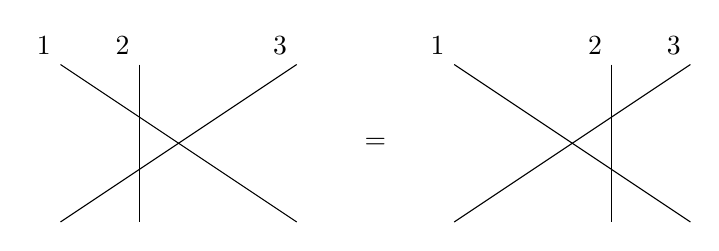
\begin{tikzpicture}
\draw (0,2) node[anchor = south east] {2} -- (0,0) ;
\draw (-1,2) node[anchor = south east] {1} -- (2,0) ; 
\draw (-1,0) -- (2,2) node[anchor = south east] {3} ;
\draw (3,1) node {=};
\draw (6,2) node[anchor = south east] {2} -- (6,0) ;
\draw (4,2) node[anchor = south east] {1} -- (7,0) ; 
\draw (4,0) -- (7,2) node[anchor = south east] {3} ;
\end{tikzpicture}
\end{center}
if we label the internal states, and sum over all their possible values, i.e.

\begin{center}
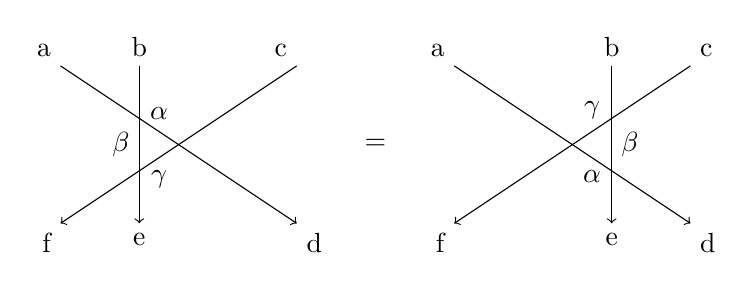
\begin{tikzpicture}

\draw[->] (0,2) node[anchor = south] {b} -- (0,0)node[anchor = north] {e} ;
\draw[->] (-1,2) node[anchor = south east] {a} -- (2,0) node[anchor = north west] {d};
\draw[->] (2,2) node[anchor = south east] {c} -- (-1,0) node[anchor = north east] {f};

\draw (0,1) node[anchor = east] {$\beta$};

\draw (0.25,1.2) node[anchor = south] {$\alpha$};

\draw (0.25,0.8) node[anchor = north] {$\gamma$};

\draw (3,1) node {=};

\draw[->] (6,2) node[anchor = south] {b} -- (6,0) node[anchor = north] {e} ;
\draw[->] (4,2) node[anchor = south east] {a} -- (7,0) node[anchor = north west] {d} ;
\draw[->] (7,2) node[anchor = south west] {c} -- (4,0) node[anchor = north east] {f};

\draw (6,1) node[anchor = west] {$\beta$};

\draw (5.75,1.2) node[anchor = south] {$\gamma$};

\draw (5.75,0.8) node[anchor = north] {$\alpha$};

\end{tikzpicture}
\end{center}

we get this indexed QYBE 
\end{remark}

\begin{prop}
$R(u) = 1 - u^{-1}P \in \End V \otimes \End V \otimes \mbb{C}(u)$ is a solution of the QYBE
\eq{
R_{12}(u-v) R_{13}(u) R_{23}(v) = R_{23}(v) R_{13}(u)R_{12}(u-v)
}
\end{prop}
\begin{proof}

Take $x,y,z \in \mbb{C}^N$. Then 
\eq{
R_{23}(v) (x \otimes y \otimes z) =& x \otimes y\otimes z + v^{-1} x \otimes z \otimes y \\
\Rightarrow R_{13}(u)R_{23}(v) (x \otimes y \otimes z) =&  x \otimes y\otimes z + v^{-1} x \otimes z \otimes y + u^{-1} z \otimes y \otimes x  + (uv)^{-1}y \otimes z \otimes x \\
\Rightarrow R_{12}(u-v) R_{13}(u) R_{23}(v)(x \otimes y \otimes z) =& x \otimes y\otimes z + v^{-1} x \otimes z \otimes y + u^{-1} z \otimes y \otimes x  + (uv)^{-1}y \otimes z \otimes x \\
& + (u-v)^{-1} y \otimes x \otimes z  + [(u-v)v]^{-1} z \otimes x \otimes y  + [(u-v)u]^{-1} y \otimes z \otimes x \\
&+ [(u-v)uv]^{-1} z \otimes y \otimes x \\
=& x \otimes y \otimes z + v^{-1} x \otimes z \otimes y + (u-v)^{-1} y \otimes x \otimes z + [(u-v)v]^{-1} y \otimes z \otimes x \\
&+ [(u-v)v]^{-1} z \otimes x \otimes y + (u^{-1} + [(u-v)uv]^{-1})z \otimes y \otimes x  
}
Alternatively 
\eq{
R_{12}(u-v)(x \otimes y \otimes z) =& x \otimes y \otimes z + (u-v)^{-1} y \otimes x \otimes z \\
\Rightarrow R_{13}(u) R_{12}(u-v) (x\otimes y \otimes z) =& x \otimes y \otimes z + (u-v)^{-1} y \otimes x \otimes z + u^{-1} z \otimes y \otimes x + [(u-v)u]^{-1} z \otimes x \otimes y \\
\Rightarrow R_{23}(v) R_{13}(u) R_{12}(u-v) (x \otimes y \otimes z) =& x \otimes y \otimes z + (u-v)^{-1} y \otimes x \otimes z + u^{-1} z \otimes y \otimes x + [(u-v)u]^{-1} z \otimes x \otimes y \\
& + v^{-1} x \otimes z \otimes y + [(u-v)v]^{-1} y \otimes z \otimes x + (uv)^{-1} z \otimes x \otimes y \\
&+ [(u-v)uv]^{-1} z \otimes y \otimes x \\
=& x \otimes y \otimes z + v^{-1} x \otimes z \otimes y + (u-v)^{-1}y \otimes x \otimes z + [(u-v)v]^{-1} y \otimes z \otimes x \\
&+ [(u-v)v]^{-1} z \otimes x \otimes y  + (u^{-1} + [(u-v)]uv)^{-1} z\otimes y \otimes x 
}
and hence done
\end{proof}

\begin{remark}
The proof above actually shows $R(u) = 1 + u^{-1} P$ is a solution, which saves on watching minus signs, but note they are equivalent as I can absorb the minus sign into the parameter $u$.
\end{remark}


Let $T(u) = 1 + u^{-1}\sum_{ij} E_{ij} \otimes E_{ij} \in \End V \otimes \mc{U}(\mf{gl}_N) \otimes \mbb{C}(u)$. We can think of it as an $N \times N$ matrix with non-commutative entries $t_{ij}(u) = \delta_{ij} + u^{-1}E_{ij}$. 

\begin{prop}
Set $T_1(u) = \sum_{ij}E_{ij} \otimes 1 \otimes t_{ij}(u), \, T_2(u) = \sum_{ij} 1 \otimes E_{ij} \otimes t_{ij}(u)$. Then 
\eq{
R_{12}(u-v)T_1(u) T_2(v) = T_2(v) T_1(u) R_{12}(u-v) \; \in \End V \otimes \End V \otimes \mc{U}(\mf{gl}_N) \otimes \mbb{C}(u,v)
}
 in, where $R$ solves the QYBE is equivalent to the commutation relations for the generators $E_{ij}$ of $\mc{U}(\mf{gl}_N)$. This is the \bam{RTT} equation 
\end{prop}
\begin{proof}
This is a restriction of the proof of lemma \ref{lemma:CQIS:YangianCommReln}. 
\end{proof}
To re-interpret the above, we can calculate
\eq{
R_{12} T_1 T_2 v^a \otimes v^b \otimes 1 &+ \sum_\beta R_{12}T_1 v^a \otimes v^\beta \otimes t^b_\beta \\
&= \sum_{\alpha,\beta} R_{12} v^\alpha \otimes v^\beta \otimes t^a_\alpha t^b_\beta  \\
&= \sum_{c,d,\alpha,\beta} R^{\alpha\beta}_{cd} v^c \otimes v^d \otimes  t^a_\alpha t^b_\beta \\
T_2 T_1 R_{12} v^a \otimes v^b \otimes 1 &= \sum_{\alpha,\beta} R_{\alpha\beta}^{ab} T_2 T_1 v^\alpha \otimes v^\beta \otimes 1 \\
&= \sum_{c,\alpha,\beta} T_2 v^c \otimes v^\beta \otimes t^\alpha_c \\
&= \sum_{c,d,\alpha,\beta} R^{ab}_{\alpha\beta} v^c \otimes v^d \otimes t^\beta_d t^\alpha_c \\ 
\Rightarrow \sum_{\alpha,\beta} R^{ab}_{\alpha\beta} t^\beta_d t^\alpha_c &= \sum_{\alpha,\beta} R^{\alpha\beta}_{cd} t^a_\alpha t^b_\beta
}


Note the above allows us to write 
\eq{
R_{12}R_{13}R_{23} T_1 T_2 T_3 = T_3 T_2 T_1 R_{12} R_{13} R_{23}
}
Doing the rearrangement in the above in different orders gives the QYBE. 

\begin{remark}
As we did with the QYBE, we can use a graphical mnemonic for the RTT relation, which looks as below 
\begin{center}
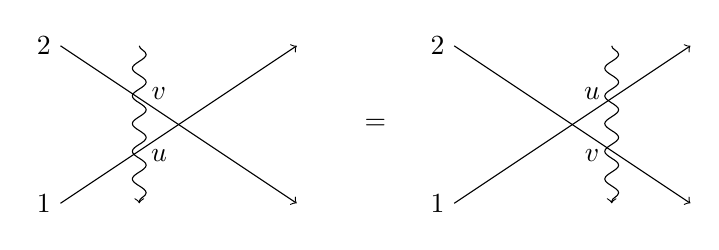
\begin{tikzpicture}
\draw[decorate, decoration=snake,->] (0,2)  -- (0,0) ;
\draw[->] (-1,2) node[anchor = east] {2} -- (2,0) ;
\draw[->] (-1,0)node[anchor = east] {1} -- (2,2)  ;

\draw (0.25,1.2) node[anchor = south] {$v$};

\draw (0.25,0.8) node[anchor = north] {$u$};

\draw (3,1) node {=};

\draw[decorate, decoration=snake,->] (6,2) -- (6,0) ;
\draw[->] (4,2) node[anchor = east] {2} -- (7,0) ; 
\draw[->] (4,0) node[anchor = east] {1} -- (7,2)  ;

\draw (5.75,1.2) node[anchor = south] {$u$};

\draw (5.75,0.8) node[anchor = north] {$v$};
\end{tikzpicture}
\end{center}
\end{remark}

We can now generalise our universal enveloping algebra:
\begin{definition}
Let $T(u) = \sum_{ij} E_{ij} \otimes t_{ij}(u)\in \End(V) \otimes Y(\mf{gl}_N) \otimes \mbb{C}[[u^{-1}]]$ where 
\eq{
t_{ij}(u) &= \delta_{ij} + \sum_{k \geq 1} t_{ij}^{(k)} u^{-k} \\
&= \sum_{k \geq 0} t_{ij}^{(k)} u^{-k} \quad \text{letting $t_{ij}^{(0)} = \delta_{ij}$}
}
The \bam{Yangian}, $Y(\mf{gl}_N)$, is the unital associative algebra with generators $\pbrace{t_{ij}^{(k)} \, | \, k \geq 1}$ and relations given by imposing the RTT relation.
\end{definition}

\begin{lemma}[Yangian commutation relations]\label{lemma:CQIS:YangianCommReln}
The $t_{ij}^{(k)}$ satisfy
\begin{enumerate}
    \item $\comm[t_{ik}^{(r+1)}]{t_{kl}^{(s)}} - \comm[t_{ik}^{(r)}]{t_{kl}^{(s+1)}} = t_{kj}^{(r)} t_{il}^{(s)} - t_{kj}^{(s)} t_{il}^{(r)}$
    \item $\comm[t_{ij}^{(r)}]{t_{kl}^{(s)}} = \sum_{m=1}^{\min(r,s)} \psquare{ t_{kj}^{(m-1)}t_{il}^{(r+s-m)} - t_{kj}^{(r+s-m)} t_{il}^{(m-1)}}$
\end{enumerate}
\end{lemma}
\begin{proof}
\hl{This is copied over from the answer to the assignment, and so needs a sign fix throughout.}
Defining $s_{ij}(u) = \delta_{ij} + u^{-1}E_{ji}$ we have $R(u) = \sum_{i,j} E_{ij} \otimes s_{ij}(u) $. As such 
\eq{
T_2(v)T_1(u)R_{12}(u-v) &= \pround{\sum_{k,l} 1 \otimes E_{kl} \otimes t_{kl}(v)}\pround{\sum_{i,j}E_{ij} \otimes 1 \otimes t_{ij}(u)}\pround{\sum_{m,n} E_{mn} \otimes s_{mn}(u-v) \otimes 1} \\
&= \sum_{i,j,k,l,m,n} (E_{ij}E_{mn}) \otimes (E_{kl}s_{mn}(u-v)) \otimes (t_{kl}(v)t_{ij}(u)) \\
&= \sum_{i,j,k,l,m,n} \delta_{jm}E_{in} \otimes (\delta_{mn}E_{kl} + (u-v)^{-1}\delta_{ln}E_{km})  \otimes (t_{kl}(v)t_{ij}(u)) \\
&= \sum_{i,j,k,l,n} E_{in} \otimes (\delta_{jn}E_{kl}+(u-v)^{-1}\delta_{ln}E_{kj}) \otimes (t_{kl}(v)t_{ij}(u))\\
&= \sum_{i,j,k,l} (E_{ij} \otimes E_{kl} + (u-v)^{-1}E_{il} \otimes E_{kj}) \otimes (t_{kl}(v)t_{ij}(u)) 
}
Similarly,
\eq{
R_{12}(u-v) T_1(u) T_2(v) &= \sum_{i,j,k,l,m,n} (E_{mn}E_{ij}) \otimes (s_{mn}(u-v) E_{kl}) \otimes (t_{ij}(u)t_{kl}(v)) \\
&= \sum_{i,j,k,l,m,n} \delta_{ni}E_{mj} \otimes (\delta_{mn}E_{kl} + (u-v)^{-1}\delta_{km}E_{nl}) \otimes (t_{ij}(u)t_{kl}(v)) \\
&= \sum_{i,j,k,l} (E_{ij} \otimes E_{kl} + (u-v)^{-1}E_{kj}\otimes E_{il}) \otimes (t_{ij}(u)t_{kl}(v))
}
This means we can write 
\eq{
R_{12}(u-v) T_1(u) T_2(v) - T_2(v)T_1(u)R_{12}(u-v) =& \sum_{i,j,k,l} 
E_{ij} \otimes E_{kl} \otimes \comm[t_{ij}(u)]{t_{kl}(v)} \\
&+ (u-v)^{-1} E_{ij} \otimes E_{kl} \otimes \psquare{t_{kj}(v)t_{il}(u) - t_{kj}(u)t_{il}(v)} \\
\Rightarrow \comm[t_{ij}(u)]{t_{kl}(v)} + (u-v)^{-1}\psquare{t_{kj}(v)t_{il}(u) - t_{kj}(u)t_{il}(v)} =& \, 0 
}
This is an equality of Laurent series, so we can compare terms of order $u^{-r}v^{-s}$ to get constraints. We will assume $u > v$ to expand $(u-v)^{-1}$ in a convergent Laurent series, but we could equally assume $v > u$ and follow through the calculation, getting the same result. We don't let $u=v$ in order to have $R(u-v)$ finite. Now 
\eq{
(u-v)^{-1} = u^{-1}\pround{1-\frac{v}{u}}^{-1} = u^{-1}\sum_{m \geq 0} \pround{\frac{v}{u}}^m = \sum_{m \geq 0} v^m u^{-m-1}
}
Thus 
\eq{
\sum_{r,s \geq 0}\comm[t_{ij}^{(r)}]{t_{kl}^{(s)}} u^{-r} v^{-s} &= -\sum_{m\geq 0} v^m u^{-m-1} \sum_{r,s \geq 0 } u^{-r}v^{-s}\psquare{t_{kj}^{(s)} t_{il}^{(r)} - t_{kj}^{(r)} t_{il}^{(s)} } 
}
and so 
\eq{
\comm[t_{ij}^{(r)}]{t_{kl}^{(s)}} = -\sum_{m \geq 0} \psquare{t_{kj}^{(s+m)} t_{il}^{(r-m-1)} - t_{kj}^{(r-m-1)} t_{il}^{(s+m)}}
}
Using that for $m <0, \, t_{ij}^{(m)} = 0$, we may rewrite and re-index the sum ($m \mapsto m-s-1$) as 
\eq{
\comm[t_{ij}^{(r)}]{t_{kl}^{(s)}} = -\sum_{m=1}^{\min(r,s)} \psquare{ t_{kj}^{(m-1)}t_{il}^{(r+s-m)} - t_{jk}^{(r+s-m)} t_{il}^{(m-1)}}
}
An immediate corollary of this is (wlog taking $s <r$)
\eq{
\comm[t_{ij}^{(r+1)}]{t_{kl}^{(s)}} - \comm[t_{ij}^{(r)}]{t_{kl}^{(s+1)}} =& -\left\lbrace\sum_{m=1}^{\min(r+1,s)} \psquare{ t_{kj}^{(m-1)}t_{il}^{(r+s+1-m)} - t_{kj}^{(r+s+1-m)} t_{il}^{(m-1)}} \right.\\
&- \left. \sum_{m=1}^{\min(r,s+1)} \psquare{ t_{kj}^{(m-1)}t_{il}^{(r+s+1-m)} - t_{kj}^{(r+s+1-m)} t_{il}^{(m-1)}} \right\rbrace \\
=&  \sum_{m=s+1}^{s+1} \psquare{ t_{kj}^{(m-1)}t_{il}^{(r+s+1-m)} - t_{kj}^{(r+s+1-m)} t_{il}^{(m-1)}} \\
=& t_{kj}^{(s)}t_{il}^{(r)} - t_{kj}^{(r)} t_{il}^{(s)}
}
\end{proof}

\begin{prop}
The map $\pi: t_{ij}(u) \mapsto \delta_{ij} + u^{-1}E_{ij}$ is an algebra epimorphism $Y(\mf{gl}_N) \to \mc{U}(\mf{gl}_N)$, and the map $i : E_{ij} \mapsto t_{ij}^{(1)}$ is an embedding $\mc{U}(\mf{gl}_N) \hookrightarrow Y(\mf{gl}_N)$. 
\end{prop}

\begin{remark}
It follows that any $\mf{gl}_N$-module can be extended to a $Y(\mf{gl}_N)$-module using $\pi$. (E.g. see lattice models later)
\end{remark}

An advantage of defining $Y$ using the RTT relation is that we can easily read off the transformations of $T(u)$ which lead to a new solution $\tilde{T}(u)$ of RTT and thus induce algebra (anti-)homomorphisms of $Y$. 

\begin{prop}
Let $f(u) \in \mbb{C}[[u^{-1}]]$, $f(\infty) = 1$, and $M$ a non-singluar matrix. The maps 
\begin{itemize}
    \item $T(u) \mapsto f(u) T(u)$
    \item $T(u) \mapsto T(u+a)$ 
    \item $T(u) \mapsto MT(u) M^{-1}$
\end{itemize}
are automorphisms of $Y$ and 
\begin{itemize}
    \item $T(u) \mapsto T(-u)$
    \item $T(u) \mapsto T(u)^T$
    \item $T(u) \mapsto T(u)^{-1}$
\end{itemize}
are anti-automorphisms. 
\end{prop}

\begin{remark}
As $T(u)$ is a formal power series in $u^{-1}$ with matrix coefficient, and the first term is the identity, it must be the case that $T^{-1}$ exists.
\end{remark}


\hl{insert section from Molev on quantum determinant}

%%%%%%%%%%%%%%%%%%%%%%%%%%%%%%%%%%%%%%%%%%%%%%%%%%%%%%%%%%%%%%%%%%%%%%%%%%%%%%%
\subsection{Hopf algebra structure}

\begin{prop}[Railroad principle]
If $T(u)$ a solution of RTT, then $\Delta (T(u)) \equiv T(u) \otimes T(u) = \pround{\sum_a t_{aj}(u) \otimes t_{ia}(u)}_{ij}$ is also a solution in $Y \otimes Y$
\end{prop}
\begin{corollary}
The map $\Delta : Y(\mf{gl}_N) \to Y(\mf{gl}_N) \otimes Y(\mf{gl}_N)$ is an algebra homomorphism
\end{corollary}

Let $A$ be an associative unital $\mbb{C}$-algebra, then the following diagram commute:

\begin{tkz}
A \otimes A \arrow[d,"m"'] & A \otimes A \otimes A \arrow[l,"m \otimes \id"'] \arrow[d,"\id \otimes m"] \\ A & A\otimes A \arrow[l,"m"]
\end{tkz}

\begin{tkz}
A \otimes A  \arrow[d,"m"'] & A \otimes \mbb{C} \arrow[l,"\id \otimes 1"'] \arrow[dl,"\sim"] \\ 
A & 
\end{tkz}
\begin{tkz}
A \otimes A  \arrow[d,"m"'] & \mbb{C} \otimes A  \arrow[l,"1 \otimes \id "'] \arrow[dl,"\sim"] \\ 
A & 
\end{tkz}

\begin{definition}
Let $A$ be a $\mbb{C}$-vector space with linear maps $\Delta : A \to A \otimes A$ (\bam{coproduct}), $\eps: A \to \mbb{C}$ (\bam{co-unit}) s.t. the co-diagrams to the above commute, i.e. 
\begin{tkz}
A \otimes A \arrow[r,"\Delta \otimes \id"] & A \otimes A \otimes A \\ 
A \arrow[u,"\Delta"] \arrow[r,"\Delta"] & A \otimes A \arrow[u,"\id \otimes \Delta"']
\end{tkz}
\begin{tkz}
A \otimes A \arrow[r,"\id \otimes \eps"] & A \otimes \mbb{C} \\
A \arrow[u,"\Delta"] \arrow[ur,"\sim"']
\end{tkz}
\begin{tkz}
A \otimes A \arrow[r,"\eps \otimes \id"] & \mbb{C} \otimes A  \\
A \arrow[u,"\Delta"] \arrow[ur,"\sim"']
\end{tkz}
Then we call $A$ a \bam{coalgebra}. If $A$ is also a unital associative algebra and $\Delta, \eps$ are algebra homormorphism the we call $A$ a \bam{bialgebra}. 
\end{definition}

\begin{remark}
Note that being a bialgebra is equivalent to being an algebra \bam{and also} a coalgebra. This links us back to our definition of Lie bialgebra, which has the additional structure of the coalgebra also being a Lie algebra. 
\end{remark}

\begin{example}
A natural example is the group algebra $\mbb{C}G$, in which elements are formal sums of group elements. Here we have 
\eq{
\Delta : \mbb{C}G &\to \mbb{C}G \otimes \mbb{C}G \\
g &\mapsto g \otimes g \\
\eps : \mbb{C}G &\to \mbb{C} \\
g &\mapsto 1
}
Note the co-product is co-commutative. Moreover,  this algebra also has the natural map $S : \mbb{C}G \to \mbb{C}G, \, g \mapsto g^{-1}$ which is an antihomomorphism. 
\end{example}

\begin{definition}
A bialgebra $H$ is called a \bam{Hopf algebra} if it also has an antihomomorphism $S : H \to H$ (called the \bam{antipode}) s.t. 
\begin{tkz}
H \otimes H \arrow[r,"S \otimes \id"] & H \otimes H \arrow[d,"m"] \\
H \arrow[u,"\Delta"] \arrow[r,"1 \circ \eps"'] & H
\end{tkz}

\begin{tkz}
H \otimes H \arrow[r,"\id \otimes S"] & H \otimes H \arrow[d,"m"] \\
H \arrow[u,"\Delta"] \arrow[r,"1 \circ \eps"'] & H
\end{tkz}

commute
\end{definition}

\begin{theorem}
The Yangian is a Hopf algebra with 
\begin{itemize}
    \item Co-product $\Delta (t_{ij}(u)) = \sum_a t_{aj}(u) \otimes t_{ia}(u)$
    \item Co-unit $\eps(t_{ij}(u)) = \delta_{ij}$
    \item Antipode $S(t_{ij}(u)) = (T^{-1}(u))_{ij}$
\end{itemize}
\end{theorem}
\begin{proof}
The hardest part is showing that $\Delta$ is a hom, which comes from the railroad principle. 
\end{proof}

\begin{remark}
There is an alternative Hopf algebra structure on the Yangian where we instead take $\Delta^\prime(t_{ij}(u)) = \sum_a t_{ia}(u) \otimes t_{aj(u)}$
\end{remark}

\begin{prop}
The map $T(u) \to T(-u)^T $ defines an involutive automorphism of $Y(\mf{gl}_N)$, $\tau_N$, which interchanges co-product on $Y$ by $\Delta^\prime \circ \tau_N = (\tau_N \otimes \tau_N) \circ \Delta$. 
\end{prop}

%%%%%%%%%%%%%%%%%%%%%%%%%%%%%%%%%%%%%
\subsection{The Yangian as a deformation of \secmath{\mc{U}(\mf{gl}_N[x])}}

Note that $Y(\mf{gl}_N)$ is a filtered algebra w.r.t. the grading $\deg t_{ij}^{(r+1)} = r$, that is if $Y_r$ is the subspace of elements of degree $\leq r$ then $Y_r Y_s \subseteq Y_{r+s}$. 

\begin{prop}
The associated graded algebra $\gr Y = \bigoplus_{r \geq 1} \faktor{Y_r}{Y_{r-1}}$ is isomorphic to $\mc{U}(\mf{gl}_N[x])$
\end{prop}
\begin{proof}
Recall the relation 
\eq{
\underbrace{\comm[t_{ij}^{(r)}]{t_{kl}^{(s)}}}_{\in Y_{r+s-2}} = \sum_{m=1}^{\min(r,s)} \psquare{ t_{kj}^{(m-1)}t_{il}^{(r+s-m)} - t_{kj}^{(r+s-m)} t_{il}^{(m-1)}} = \underbrace{\delta_{kj}t_{il}^{(r+s-1)} - \delta_{il}t_{kj}^{r+s-1}}_{\in Y_{r+s-2}} + \underbrace{\dots}_{\in Y_{r+s-3}}
}
and so the map 
\eq{
\mc{U}(\mf{gl}_N[x]) &\to \gr Y \\
E_{ij}x^{r-1} &\mapsto t_{ij}^{(r)}+ Y_{r-2}
}
is an algebra epimorphism. Since any element in $Y$ can be uniquely written as a linear combination of monomials in the generators $t_{ij}^{(r)}$, the kernel of this map must be trivial. 
\end{proof}

\begin{remark}
This map extends to an isomorphism of Hopf algebras with $\forall g \in \mf{gl}_N[x], \, \Delta(g) = g \otimes 1 + 1 \otimes g$, $\eps(g) = 0$, $S(g) = -g$
\end{remark}

\begin{remark}
The statement that "any element in $Y$ can be uniquely written as a linear combination of monomials in the generators $t_{ij}^{(r)}$" is not entirely trivial, but is a consequence of the Poincar\'e-Birkhoff-Witt theorem. 
\end{remark}

%%%%%%%%%%%%%%%%%%%%%%%%%%%%%%%%%%%%%
%%%%%%%%%%%%%%%%%%%%%%%%%%%%%%%%%%%%
\section{Lattice models in statistical mechanics}

Let $G$ be an $m \times n$ square lattice. Denote by $E(G)$ the set of its edges and $V(G)$ the set of its vertices $v = \pangle{i,j}$. Given a vertex, denote by $N,E,S,W$ its adjacent north, east, south, and west edges respectively. Fix some $\bm{\lambda} = (\lambda_1, \dots, \lambda_m)\in \mbb{C}^m, \, \bm{\mu} = (\mu_1, \dots, \mu_n)\in \mbb{C}^n$

\begin{definition}
A \bam{lattice configuration} is a map $\gamma : E(G) \to \pbrace{1, \dots, N} \equiv [N]$ \\
Denote $\Gamma$ the set of all lattice configurations for a given $R$-matrix $R(\bm{\lambda},\bm{\mu}) : \mbb{C}^N \otimes C^N \to \mbb{C}^N \otimes \mbb{C}^N$
\end{definition}

\begin{remark}
The purpose of this definition of a lattice configuration is such that we imagine the following picture 
\begin{center}
    \begin{tikzpicture}
    \draw[->,text=red] (-1,0) node[anchor = south] {$\lambda_1$} -- (4,0);
    \draw[->,text=red] (-1,1) node[anchor = south] {$\lambda_2$} -- (4,1);
    \draw[text=red] (-1.15,2) node [anchor = south] {$\vdots$};
    \draw[->,text = red] (-1,3) node[anchor = south] {$\lambda_m$} -- (4,3);
    
    \draw[->,text=red] (0,4) -- (0,-1) node[anchor = west] {$\mu_1$};
    \draw[->,text=red] (1,4) -- (1,-1) node[anchor = west] {$\mu_2$};
    \draw[text=red] (2,-1) node [anchor = west] {$\cdots$};
    \draw[->,text=red] (3,4) -- (3,-1) node[anchor = west] {$\mu_n$};
    \end{tikzpicture}
\end{center}
wherein each vertex corresponds to a scattering via an $R$ matrix as 
\begin{center}
    \begin{tikzpicture}
    \draw[->] (-1,0) node[anchor = east] {i}  -- (1,0) node[anchor = west] {k} ;
    \draw[->] (0,1) node[anchor = south] {j} -- (0,-1) node[anchor = north] {l};
    \draw[text=red]  (-1,0) node[anchor=south] {$\lambda_a$};
    \draw[text=red] (0,-1) node[anchor=east] {$\mu_b$};
    
    \draw (2,0) node {$\sim$} ;
    
    \draw (2.5,0) node[anchor = west] {$R^{ij}_{kl}(\lambda_a - \mu_b)$};
    
    \end{tikzpicture}
\end{center}
I like to think of this as two states, $i,j$ going in, and coming out at $k,l$ with a new factor in front of them (very akin to how we visualise scattering, hence the use of the language). The red text identifies the rep space the vertex lives in, while the indices in black at the end of the lines tell us the state coming in or out. 
\end{remark}

\begin{definition}
The \bam{weight} of a lattice configuration is
\eq{
\wt_{\bm{\lambda},\bm{\mu}} : \Gamma &\to \mbb{C} \\
\gamma &\mapsto \prod_{\pangle{i,j}\in V(G)} R^{\gamma(S) \gamma(E)}_{\gamma(N) \gamma(W)}(\lambda_i,\mu_j)
}
\hl{1: this doesn't agree with the diagram above, so solve this issue}
\end{definition}

\begin{definition}
The \bam{partition function} is the weighted sum over all the lattice configurations 
\eq{
Z(\bm{\lambda},\bm{\mu}) = \sum_{\gamma \in \Gamma} \wt(\gamma)
}
\end{definition}

\begin{remark}
Note that we have freedom to rescale our $R$ matrix by a constant. Hence if we can scale s.t, for fixed $\bm{\lambda},\bm{\mu}$, $Z=1$, then we interpret $\wt(\gamma)$ as the probability of a given lattice configuration $\gamma$. In statistical mechanics the partition function is the main ingredient in working out what happens, and so if we can work it out, we are sorted (\hl{ maybe include an example of this? I've never done statistical mechanics so should include at least one})
\end{remark}

%%%%%%%%%%%%%%%%%%%%%%%%%%%%%%%%%%%%%%%%%%%%%%%%%%%%%%%%%%%%%%%%%%%%%%%%%%
\subsection{Evaluation modules}

Recall the two algebra homomorphisms 
\eq{
Y(\mf{gl}_N) &\to \mc{U}(\mf{gl}_N) \\
t_{ij}(u) &\mapsto \delta_{ij}I + u^{-1}E_{ij} \\
&\phantom{\to} \\
Y(\mf{gl}_N) &\to Y(\mf{gl}_N) \\
t_{ij}(u) &\mapsto t_{ij}(u - \mu)
}
where $\mu \in \mbb{C}$.

\begin{remark}
Note here I am being lazy and these are actually maps from $Y(\mf{gl}_N)[[u^{-1}]]$. 
\end{remark}

Hence, given a $\mf{gl}_N$-module $V$,  we may define the $Y(\mf{gl}_N)$-module $V(\mu)$ with the action  
\eq{
t_{ij}(u) \cdot v \equiv \psquare{\delta_{ij}I + (u - \mu)^{-1}E_{ij}} \cdot v
}
Let us write this as $t_{ij}(u) \mapsto \delta_{ij} + (u - \mu)^{-1}E_{ij}$.
Note that if $V = \mbb{C}^N$ with the fundamental rep, then this is the rep that acts as 
\eq{
T(u) \mapsto T_{V(\mu)}(u) = R(u-\mu) \in \End(V^{\otimes 2}) \cong (\End \mbb{C}^N)^{\otimes 2}
}

\begin{remark}
\hl{2: I have written this down, but now I do not believe it.} We consider $T_{V(\mu)}$ as a matrix with entries $\delta_{ij} + (u-\mu)^{-1}E_{ij}$, but $R(u-\mu)$ is a matrix with entries $\delta_{ij} - (u-\mu)^{-1}E_{ji}$!
\end{remark}

\begin{remark}
As $R$ solves the QYBE, $T$ as defined above solves the RTT relation. 
\end{remark}

We can then 'upgrade' to a lattice model by considering the module $V(\mu_1) \otimes \dots \otimes V(\mu_n)$. 

\begin{definition}\label{def:CQIS:monodromymatrix}
The \bam{row-to-row monodromy matrix} is
\eq{
T_{\bigotimes_{i=1}^n V(\mu_i)} (\lambda_a) = T(\lambda_a,\bm{\mu}) = R_{an}(\lambda_a - \mu_n) \dots R_{a1}(\lambda_a - \mu_1) \in \End \psquare{V(\lambda_a) \otimes \bigotimes_{i=1}^n V(\mu_i)}
}
for the $a^{th}$ row. It can be represented as an $N \times N$ matrix with entries $t_{ij}(\lambda_a,\bm{\mu})$ called the \bam{row-to-row transfer matrices}. Graphically we view the row-to-row transfer matrices as  
\begin{center}
    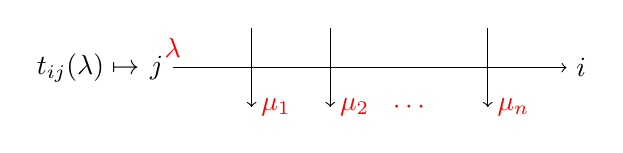
\begin{tikzpicture}
    \draw (-2.3,0) node[anchor = east] {$t_{ij}(\lambda) \mapsto$};
    \draw[->] (-2,0) node[anchor = east] {$j$} -- (3,0) node[anchor = west] {$i$};
    \draw[text=red] (-2,0) node[anchor = south] {$\lambda$};
    \draw[->,text=red] (-1,0.5) -- (-1,-0.5) node[anchor = west] {$\mu_1$} ;
    \draw[->,text=red] (0,0.5) -- (0,-0.5) node[anchor = west] {$\mu_2$} ;
    \draw[text=red] (1,-0.5) node {$\cdots$};
    \draw[->,text=red] (2,0.5) -- (2,-0.5) node[anchor = west] {$\mu_n$} ;
    \end{tikzpicture}
\end{center}
With this we can define the \bam{monodromy matrix}
\eq{
T(\bm{\lambda},\bm{\mu}) = R_{1n}(\lambda_1,\mu_n) \dots R_{11}(\lambda_1, \mu_1) \dots R_{mn}(\lambda_m,\mu_n) \dots R_{m1}(\lambda_m,\mu_1) \in \End \psquare{\bigotimes_{a=1}^m V(\lambda_m) \otimes \bigotimes_{i=1}^n V(\mu_i)}
}
which corresponds to the picture
\begin{center}
    \begin{tikzpicture}
    \draw[->,text=red] (-1,0) node[anchor = south] {$\lambda_1$} -- (4,0);
    \draw[->,text=red] (-1,1) node[anchor = south] {$\lambda_2$} -- (4,1);
    \draw[text=red] (-1.15,2) node [anchor = south] {$\vdots$};
    \draw[->,text = red] (-1,3) node[anchor = south] {$\lambda_m$} -- (4,3);
    
    \draw[->,text=red] (0,4) -- (0,-1) node[anchor = west] {$\mu_1$};
    \draw[->,text=red] (1,4) -- (1,-1) node[anchor = west] {$\mu_2$};
    \draw[text=red] (2,-1) node [anchor = west] {$\cdots$};
    \draw[->,text=red] (3,4) -- (3,-1) node[anchor = west] {$\mu_n$};
    \end{tikzpicture}
\end{center}

\end{definition}

\begin{lemma}\label{lemma:CQIS:PartitionFnFromMonodromy}
Let $\bm{a} \in [N]^{\times m}, \, \bm{b} \in [N]^{\times n }$, then 
\eq{
T(\bm{\lambda},\bm{\mu}) \pround{ \bigotimes_{i=1}^m v^{a_i}} \otimes \pround{ \bigotimes_{j=1}^n v^{b_j}} = \sum_{\bm{c},\bm{d}} Z^{\bm{a}\bm{b}}_{\bm{c}\bm{d}}(\bm{\lambda},\bm{\mu})\pround{ \bigotimes_{i=1}^m v^{c_i}} \otimes \pround{ \bigotimes_{j=1}^n v^{d_j}}
}
where 
\eq{
Z^{\bm{a}\bm{b}}_{\bm{c}\bm{d}}(\bm{\lambda},\bm{\mu}) = \sum_{\gamma \in \Gamma^{\bm{a}\bm{b}}_{\bm{c}\bm{d}}} \wt(\gamma)
}
for 
\eq{
\Gamma^{\bm{a}\bm{b}}_{\bm{c}\bm{d}} = \pbrace{\gamma : E(G) \to [N] \, | \, \gamma(i,0) = a_i, \, \gamma(i,n) = c_i, \, \gamma(1,j) = d-j, \, \gamma(m,j) = b_j}
}
\end{lemma}

\begin{remark}
We can see the lattice configurations $\Gamma^{\bm{a}\bm{b}}_{\bm{c}\bm{d}}$ pictorially as 
\begin{center}
    \begin{tikzpicture}
        \draw (-1,0) node[anchor = east] {$a_1$} -- (4,0) node[anchor = west] {$c_1$};
    \draw (-1,1) node[anchor = east] {$a_2$} -- (4,1) node[anchor = west] {$c_2$};
    \draw (-1.15,2) node [anchor = east] {$\vdots$};
    \draw (4.15,2) node [anchor = west] {$\vdots$};
    \draw (-1,3) node[anchor = east] {$a_m$} -- (4,3) node[anchor = west] {$c_m$};
    
    \draw (0,4) node[anchor=south] {$b_1$}-- (0,-1) node[anchor = north] {$d_1$};
    \draw (1,4) node[anchor=south] {$b_2$} -- (1,-1) node[anchor = north] {$d_2$};
    \draw (2,-1) node [anchor = north] {$\cdots$};
    \draw (2,4) node [anchor = south] {$\cdots$};
    \draw (3,4) node[anchor=south] {$b_n$} -- (3,-1) node[anchor = north] {$d_n$};
    \end{tikzpicture}
\end{center}
\end{remark}

\begin{lemma} We have 
\eq{
\sum_{k,l} R^{kl}_{c_i c_{i+1}}(\lambda_i, \lambda_{i+1}) Z^{\bm{a}\bm{b}}_{(c_1, \dots, k,l, \dots, c_m)\bm{d}}(\bm{\lambda},\bm{\mu}) = \sum_{k,l} Z^{(a_1, \dots, k,l, \dots, a_m)\bm{b}}_{\bm{c}\bm{d}}(\dots, \lambda_{i+1}, \lambda_i, \dots, \bm{\mu}) R_{kl}^{a_i a_{i+1}}(\lambda_i, \lambda_{i+1})
}
\end{lemma}
\begin{proof}
Apply the RTT relation \hl{and finish this / exercise}
\end{proof}

\begin{remark}
Note that when $m=1$, this reduces to the partition function for a single row, and $T$ reduces to the solution of the standard RTT relation we know. 
\end{remark}

\begin{lemma}
$T(\bm{\lambda},\bm{\mu}) = T_1(\lambda_1,\bm{\mu}) \cdots T_m(\lambda_m,\bm{\mu})$
\end{lemma}

\begin{lemma}
We can restate lemma \ref{lemma:CQIS:PartitionFnFromMonodromy} in terms of the transfer matrices as 
\eq{
t_{a_1 c_1}(\lambda_1, \bm{\mu})t_{a_2 c_2}(\lambda_2, \bm{\mu}) \cdots t_{a_m c_m}(\lambda_m, \bm{\mu}) \bigotimes_{j=1}^n e^{b_j} = \sum_{\bm{d}} Z^{\bm{a}\bm{b}}_{\bm{c}\bm{d}}(\bm{\lambda},\bm{\mu}) \bigotimes_{j=1}^n e^{d_j}
}
\end{lemma}

%%%%%%%%%%%%%%%%%%%%%%%%%%%%%%%%%%%%%
\subsection{Special Cases: Periodic Boundary Conditions}
Let $\Gamma_{ij}$ be the set of lattice configurations where the right/left outer horizontal edges have values $i/j$. We assume periodic boundary conditions in the vertical directions. Graphically that is 
\begin{center}
    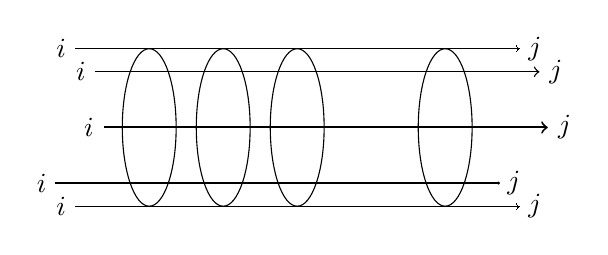
\begin{tikzpicture}
    \def\t{70}
    \def\a{45}
    \def\m{-2}
    \def\e{4}
    \foreach \n in {0,1,2,\e}
    {
    \draw ({\m+\n*sin(\t)},0) ellipse ({cos(\t)} and 1);
    }
    \foreach \k in {0,1,2,4,5} 
    {
    \draw[->][line width = {0.7*sin(\k*\a)} ] ({\m+sin(\k*\a)*cot(\t)-sin(\t)},{cos(\k*\a)}) node[anchor = east] {$i$} -- ({\m+(\e+1)*sin(\t)+sin(\k*\a)*cot(\t)},{cos(\k*\a)}) node[anchor = west] {$j$} ;
    }
    \end{tikzpicture}
\end{center}

\begin{lemma}
$\tr t_{ij}^m(\lambda,\bm{\mu}) = \sum_{\gamma \in \Gamma_{ij}} \wt_{\lambda,\bm{\mu}}(\gamma)$
\end{lemma}

\begin{lemma}
If $R(\lambda,\lambda^\prime)$ is invertible the the partition function for the cylinder 
\eq{
Z_{cyl}(\bm{\lambda},\bm{\mu}) = \sum_{\bm{a}} Z_{\bm{a}\bm{d}}^{\bm{a}\bm{c}}(\bm{\lambda},\bm{\mu})
}
is symmetric in the $\lambda_i$. In particular, row-to-row transfer matrices 
\eq{
\tau(\lambda_i,\bm{\mu}) = \tr_{\mbb{C}^N} T(\lambda_i,\bm{\mu}) = \sum_{a=1}^N t_{aa}(\lambda_i,\bm{\mu})
}
pairwise commute. 
\end{lemma}

Note that if instead of $\lambda\in \mbb{C}$ we had the formal parameter $u \in \mbb{C}(u)$, the same result may be derived. Hence expanding $\tau(u,\bm{\mu}) = \sum_{r \geq 0} u^{-r} \tau^{(r)}$, the $\tau^{(r)} \in \End \pround{\otimes V(\mu_j)}$ generate a commuting subalgebra

\hl{3: This definition is not exactly what is written in the notes where there is $u^r$ instead for the definition of the $\tau^{(r)}$. I am not sure that is correct.}

\begin{definition}
The algebra generated by the $\tau^{(r)}$ is called the \bam{Bethe algebra}.
\end{definition}

%%%%%%%%%%%%%%%%%%%%%%%%%%%%%%%%%%%%%
\subsection{Algebraic Bethe ansatz for \secmath{Y(\mf{gl}_2)} and the Heisenberg model}

A question we could now ask is whether the $\tau^{(r)}$ are simultaneously diagonalisable \hl{why would we ask this?}. We will see that in the case $N=2$ this is true, and the way to construct the solution is via a certain ansatz for the solution. This will allow us to solve a certain lattice model.  \\
Let us decompose 
\eq{
\mf{gl}_2 = \mf{n}^+ \oplus \mf{h} \oplus \mf{n}^-
}
where 
\eq{
\mf{n}^+ &= \mbb{C} E_{12} = \mbb{C}\begin{psmallmatrix} 0 & 1\\ 0 & 0 \end{psmallmatrix} \\
\mf{n}^- &= \mbb{C} E_{21} = \mbb{C}\begin{psmallmatrix} 0 & 0\\ 1 & 0 \end{psmallmatrix} \\
\mf{h} &= \mbb{C} E_{11} \oplus \mbb{C} E_{22} = \mbb{C}\begin{psmallmatrix} 1 & 0\\ 0 & 0 \end{psmallmatrix} \oplus \mbb{C}\begin{psmallmatrix} 0 & 0\\ 0 & 1 \end{psmallmatrix}
}

\begin{definition}
The \bam{quantum determinant} of $T(u) \in Y$ is 
\eq{
q\det T(u) = t_{11}(u) t_{22}(u) - t_{12}(u) t_{21}(u)
}
\end{definition}

\begin{fact}
The quantum determinant is a central element of $Y$
\end{fact}
\hl{Would like to have a simple-ish proof of this fact}

\begin{definition}
The \bam{Bethe subalgebra} is $B \subset Y$ generated by the coefficients in the Laurent series of $q\det T(u) $ and $\tr T(u) = t_{11}(u) + t_{22}(u)$.
\end{definition}

\begin{remark}
\hl{How does this connect with our previous definition in terms of the $\tau^{(r)}$?} 
\end{remark}

\begin{prop}
The Bethe subalgebra commutes with the image of the UEA under the evaluation homomorphism. 
\end{prop}
\begin{proof}
Note from our previously worked out commutation relations we have 
\eq{
\comm[t_{11}^{(r)}+t_{22}^{(r)}]{t_{ij}^{(1)}} &= \sum_{m=1}^{\min(1,r)}\psquare{t_{i1}^{(m-1)}t_{1j}^{(r+1-m)} - t_{i1}^{(r+1-m)}t_{1j}^{(m-1)} +t_{i2}^{(m-1)}t_{2j}^{(r+1-m)} - t_{i2}^{(r+1-m)}t_{2j}^{(m-1)}} \\
&=t_{i1}^{(0)}t_{1j}^{(r)} - t_{i1}^{(r)}t_{1j}^{(0)} +t_{i2}^{(0)}t_{2j}^{(r)} - t_{i2}^{(r)}t_{2j}^{(0)}
}
We can then simply check cases
\eq{
\comm[t_{11}^{(r)}+t_{22}^{(r)}]{t_{11}^{(1)}} &= t_{11}^{(r)} - t_{11}^{(r)} = 0 \\
\comm[t_{11}^{(r)}+t_{22}^{(r)}]{t_{12}^{(1)}} &= t_{12}^{(r)} - t_{12}^{(r)} =0\\
\comm[t_{11}^{(r)}+t_{22}^{(r)}]{t_{21}^{(1)}} &= - t_{21}^{(r)} +t_{21}^{(r)} =0\\
\comm[t_{11}^{(r)}+t_{22}^{(r)}]{t_{22}^{(1)}} &=  t_{22}^{(r)} +t_{22}^{(r)}=0 
}
We are given that the quantum determinant lies in the centre of $Y$, and so necessarily commutes with the Bethe subalgebra
\end{proof}

We will now restrict to the evaluation module $\bigotimes_{j=1}^n V(\mu_j)$ with $V = \mbb{C}^2$, and let $\pbrace{e_0,e_1}$ be the standard basis of $\mbb{C}^2$ (where we are now relabelling $1,2 \mapsto 0,1$). Following the convention in physics literature, re-write 
\eq{
 \begin{pmatrix} t_{00}(u) & t_{01}(u) \\ t_{10}(u) & t_{11}(u) \end{pmatrix} \mapsto T(u,\bm{\mu}) = \begin{pmatrix} A(u,\bm{\mu}) & B(u,\bm{\mu}) \\ C(u,\bm{\mu}) & D(u,\bm{\mu}) \end{pmatrix} \in \End\pround{\bigotimes_{j=1}^n V(\mu_j)}
}

\begin{lemma}
The evaluation module $\bigotimes_{j=1}^n V(\mu_j)$ is the highest weight representation of $Y(\mf{gl}_2)$ with highest weight vector $\Omega = e_0 \otimes \dots \otimes e_0$ and relations 
\eq{
A(\lambda,\bm{\mu}) \Omega &= \prod_{j=1}^n \psquare{1-(\lambda - \mu_j)^{-1}}\Omega \\
D(\lambda, \bm{\mu}) \Omega &= \Omega \\
C(\lambda,\bm{\mu}) \Omega &= 0
}
\end{lemma}
\begin{proof}
Recall graphically we wrote 
\begin{center}
    \begin{tikzpicture}
    \draw[->] (-1,0) node[anchor = east] {i}  -- (1,0) node[anchor = west] {k} ;
    \draw[->] (0,1) node[anchor = south] {j} -- (0,-1) node[anchor = north] {l};
    \draw[text=red]  (-1,0) node[anchor=south] {$\lambda_a$};
    \draw[text=red] (0,-1) node[anchor=east] {$\mu_b$};
    
    \draw (2,0) node {$\sim$} ;
    
    \draw (2.5,0) node[anchor = west] {$R^{ij}_{kl}(\lambda_a - \mu_b)$};
    
    \end{tikzpicture}
\end{center}

Hence we can explicitly list the different vertex options. Recalling that 
\eq{
R(\lambda)(e_i \otimes e_j) = e_i \otimes e_j - \lambda^{-1} e_j \otimes e_i
}
we can explicitly write the non-zero vertices as 
\begin{center}
    \begin{tikzpicture}
    \def\O{2.5}
    \def\D{-2}
    \foreach \x/\y/\i/\j/\k/\l\v in {-\O/0/0/0/0/0/$1-\lambda^{-1}$,\O/0/1/1/1/1/$1-\lambda^{-1}$,%
    -\O/\D/0/1/0/1/1/1,\O/\D/1/0/1/0/1/1,%
    -\O/{2*\D}/1/0/0/1/$\lambda^{-1}$,\O/{2*\D}/0/1/1/0/$\lambda^{-1}$}
    {
    \draw[->] ({-0.5+\x},\y) node[anchor = east] {\i}  -- ({0.5+\x},\y) node[anchor = west] {\k} ;
    \draw[->] (\x,{0.5+\y}) node[anchor = south] {\j} -- (\x,{-0.5+\y}) node[anchor = north] {\l};
    \draw ({\x+1.35},\y) node {$\sim$} ;
    \draw ({\x+1.7},\y) node[anchor = west] {\v};
    }
    \end{tikzpicture}
\end{center}
Observe these are split into 3 pair, those with identity and swap contribution, those with identity contribution, and those with swap contribution. \\
Now using $T(\lambda,\bm{\mu}) = R_{0n}(\lambda,\mu_n) \dots R_{01}(\lambda,\mu_1)$ (\hl{which I currently doubt. I think we want a transpose for the $T$ at least, and this explains the problem with C, see below.}) we associate with the the calculation of $A(\lambda,\bm{\mu})\Omega$ (remembering definition \ref{def:CQIS:monodromymatrix}) the graphic 
\begin{center}
    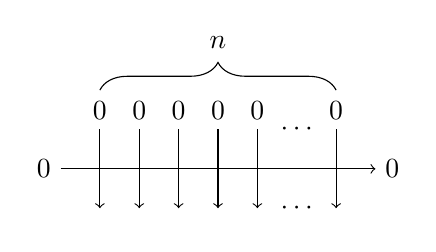
\begin{tikzpicture}
    \draw[->] (-1.5,0) node[anchor = east] {$0$} -- (2.5,0) node[anchor = west] {$0$};
    \draw[->] (-1,0.5) node[anchor = south] {$0$} -- (-1,-0.5)  ;
    \draw[->] (1,0.5) node[anchor = south] {$0$} -- (1,-0.5)  ;
    \draw[->] (-0.5,0.5) node[anchor = south] {$0$} -- (-0.5,-0.5)  ;
    \draw[->] (0.5,0.5) node[anchor = south] {$0$} -- (0.5,-0.5)  ;
    \draw[->] (0,0.5) node[anchor = south] {$0$}-- (0,-0.5)  ;
    \draw (1.5,0.5) node {$\cdots$};
    \draw (1.5,-0.5) node {$\cdots$};
    \draw[->] (2,0.5) node[anchor = south] {$0$} -- (2,-0.5) ;
    \draw[decorate, decoration={brace,amplitude=10pt},yshift=0.5cm,xshift=0pt] (-1,0.5) -- (2,0.5)  node [black,midway,yshift=0.6cm]
{$n$};
    \end{tikzpicture}
\end{center}
Using our vertex rules above we see the only non-zero output is 
\begin{center}
    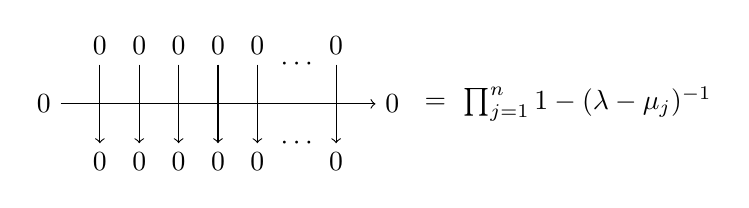
\begin{tikzpicture}
    \draw[->] (-1.5,0) node[anchor = east] {$0$} -- (2.5,0) node[anchor = west] {$0$};
    \draw[->] (-1,0.5) node[anchor = south] {$0$} -- (-1,-0.5) node[anchor = north] {$0$}  ;
    \draw[->] (1,0.5) node[anchor = south] {$0$} -- (1,-0.5) node[anchor = north] {$0$}  ;
    \draw[->] (-0.5,0.5) node[anchor = south] {$0$} -- (-0.5,-0.5) node[anchor = north] {$0$} ;
    \draw[->] (0.5,0.5) node[anchor = south] {$0$} -- (0.5,-0.5) node[anchor = north] {$0$} ;
    \draw[->] (0,0.5) node[anchor = south] {$0$}-- (0,-0.5) node[anchor = north] {$0$} ;
    \draw (1.5,0.5) node {$\cdots$};
    \draw (1.5,-0.5) node {$\cdots$};
    \draw[->] (2,0.5) node[anchor = south] {$0$} -- (2,-0.5) node[anchor = north] {$0$};
    \draw (3,0) node[anchor = west] {=} ;
    \draw (3.5,0) node[anchor = west] {$\prod_{j=1}^n\psquare{1- (\lambda-\mu_j)^{-1}}$};
    \end{tikzpicture}
\end{center}
Similarly, we know that for $D(\lambda,\bm{\mu})\Omega$ we will get the non-zero term 

\begin{center}
    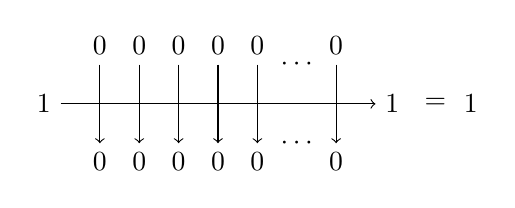
\begin{tikzpicture}
    \draw[->] (-1.5,0) node[anchor = east] {$1$} -- (2.5,0) node[anchor = west] {$1$};
    \draw[->] (-1,0.5) node[anchor = south] {$0$} -- (-1,-0.5) node[anchor = north] {$0$}  ;
    \draw[->] (1,0.5) node[anchor = south] {$0$} -- (1,-0.5) node[anchor = north] {$0$}  ;
    \draw[->] (-0.5,0.5) node[anchor = south] {$0$} -- (-0.5,-0.5) node[anchor = north] {$0$} ;
    \draw[->] (0.5,0.5) node[anchor = south] {$0$} -- (0.5,-0.5) node[anchor = north] {$0$} ;
    \draw[->] (0,0.5) node[anchor = south] {$0$}-- (0,-0.5) node[anchor = north] {$0$} ;
    \draw (1.5,0.5) node {$\cdots$};
    \draw (1.5,-0.5) node {$\cdots$};
    \draw[->] (2,0.5) node[anchor = south] {$0$} -- (2,-0.5) node[anchor = north] {$0$};
    \draw (3,0) node[anchor = west] {=} ;
    \draw (3.5,0) node[anchor = west] {$1$};
    \end{tikzpicture}
\end{center}

and for $C(\lambda,\bm{\mu})\Omega$ we get the graphic 

\begin{center}
    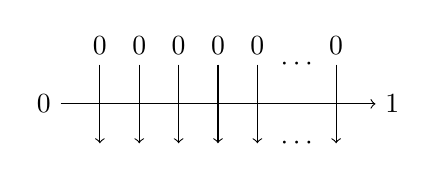
\begin{tikzpicture}
    \draw[->] (-1.5,0) node[anchor = east] {$0$} -- (2.5,0) node[anchor = west] {$1$};
    \draw[->] (-1,0.5) node[anchor = south] {$0$} -- (-1,-0.5)  ;
    \draw[->] (1,0.5) node[anchor = south] {$0$} -- (1,-0.5)  ;
    \draw[->] (-0.5,0.5) node[anchor = south] {$0$} -- (-0.5,-0.5)  ;
    \draw[->] (0.5,0.5) node[anchor = south] {$0$} -- (0.5,-0.5)  ;
    \draw[->] (0,0.5) node[anchor = south] {$0$}-- (0,-0.5)  ;
    \draw (1.5,0.5) node {$\cdots$};
    \draw (1.5,-0.5) node {$\cdots$};
    \draw[->] (2,0.5) node[anchor = south] {$0$} -- (2,-0.5) ;
    \end{tikzpicture}
\end{center}

which we can see from our graphical rules will give $0$ contribution. 
\end{proof}

\begin{remark}
\hl{4: In order to make the previous proof work} I have treated $t_{10}\mapsto B, \, t_{01} \mapsto C$ as the correct labelling. I will continue with this labelling for the rest of the section.  
\end{remark}

\begin{remark}
If you are like me and have only seen the concept of a highest weight representation in the context of Kac-Moody Lie algebras where there are obvious raising/lowering operators, you may be wondering what they are here. \hl{I would like to find out}.  
\end{remark}

With this previous result we can now state the following claim:

\begin{prop}
Let $v(\bm{\xi}) = B(\xi_1,\bm{\mu}) \cdots B(\xi_k,\bm{\mu})\Omega$ where the parameters $\bm{\xi}$ satisfy 
\eq{
\prod_{j=1}^n \frac{\xi_i -\mu_j - 1}{\xi_i - \mu_j} = \prod_{l \neq i}^k \frac{\xi_i - \xi_l + 1}{\xi_i - \xi_l - 1}
}
Then 
\eq{
\psquare{A(\lambda,\bm{\mu}) + D(\lambda,\bm{\mu})}v(\bm{\xi}) = \pround{\prod_{j=1}^n \frac{\lambda -\mu_j - 1}{\lambda - \mu_j} \prod_{l =1}^k \frac{\lambda - \xi_l + 1}{\lambda - \xi_l }+ \prod_{l=1 }^k \frac{\lambda - \xi_l - 1}{\lambda - \xi_l }} v(\bm{\xi})
}
\end{prop}
\begin{proof}
Let us supress the $\bm{\mu}$ in notation as we know which rep space we are in. We see $B(\xi)\Omega$ is graphically 
\begin{center}
    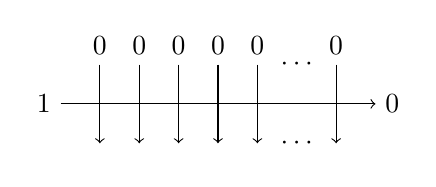
\begin{tikzpicture}
    \draw[->] (-1.5,0) node[anchor = east] {$1$} -- (2.5,0) node[anchor = west] {$0$};
    \draw[->] (-1,0.5) node[anchor = south] {$0$} -- (-1,-0.5)  ;
    \draw[->] (1,0.5) node[anchor = south] {$0$} -- (1,-0.5)  ;
    \draw[->] (-0.5,0.5) node[anchor = south] {$0$} -- (-0.5,-0.5)  ;
    \draw[->] (0.5,0.5) node[anchor = south] {$0$} -- (0.5,-0.5)  ;
    \draw[->] (0,0.5) node[anchor = south] {$0$}-- (0,-0.5)  ;
    \draw (1.5,0.5) node {$\cdots$};
    \draw (1.5,-0.5) node {$\cdots$};
    \draw[->] (2,0.5) node[anchor = south] {$0$} -- (2,-0.5) ;
    \end{tikzpicture}
\end{center}
A little bit of thinking gives that the non-zero sums come from terms like 
\begin{center}
    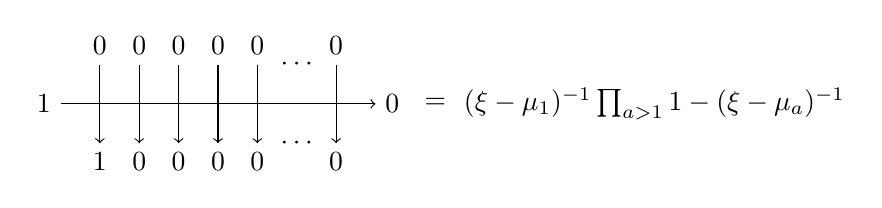
\begin{tikzpicture}
    \def\t{0.5}
    \def\s{-1.5}
    \def\k{1}
    \def\l{5}
    \def\ans{$(\xi-\mu_1)^{-1}\prod_{a > 1}\psquare{1-(\xi-\mu_a)^{-1}}$}
    \foreach \le/\ri/\y in {1/0/1} {
    \draw[->] (\s,\t-0.5*\y) node[anchor = east] {\le} -- ({\s+0.5*(\l+3)},\t-0.5*\y) node[anchor = west] {\ri};
    }
    \foreach \e/\x in {1/1,0/2,0/3,0/4,0/5,0/7} {
    \draw[->] ({\s+0.5*\x},\t) node[anchor = south] {$0$} -- ({\s+0.5*\x},{\t-0.5*(\k+1)}) node[anchor = north] {\e}  ;
    }
    \draw ({\s+0.5*(\l+1)},\t) node {$\cdots$};
    \draw ({\s+0.5*(\l+1)},{\t-0.5*(\k+1)}) node {$\cdots$};
    \draw ({\s+0.5*(\l+4)},{\t - 0.25*(\k+1)}) node[anchor = west] {=} ;
    \draw ({\s+0.5*(\l+5)},{\t - 0.25*(\k+1)}) node[anchor = west] {\ans};
    \end{tikzpicture}
\end{center}
\begin{center}
    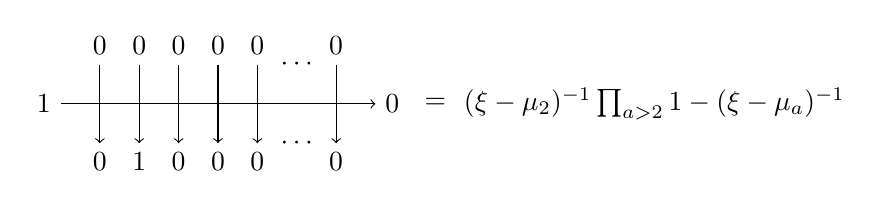
\begin{tikzpicture}
    \def\t{0.5}
    \def\s{-1.5}
    \def\k{1}
    \def\l{5}
    \def\ans{$(\xi-\mu_2)^{-1}\prod_{a > 2}\psquare{1-(\xi-\mu_a)^{-1}}$}
    \foreach \le/\ri/\y in {1/0/1} {
    \draw[->] (\s,\t-0.5*\y) node[anchor = east] {\le} -- ({\s+0.5*(\l+3)},\t-0.5*\y) node[anchor = west] {\ri};
    }
    \foreach \e/\x in {0/1,1/2,0/3,0/4,0/5,0/7} {
    \draw[->] ({\s+0.5*\x},\t) node[anchor = south] {$0$} -- ({\s+0.5*\x},{\t-0.5*(\k+1)}) node[anchor = north] {\e}  ;
    }
    \draw ({\s+0.5*(\l+1)},\t) node {$\cdots$};
    \draw ({\s+0.5*(\l+1)},{\t-0.5*(\k+1)}) node {$\cdots$};
    \draw ({\s+0.5*(\l+4)},{\t - 0.25*(\k+1)}) node[anchor = west] {=} ;
    \draw ({\s+0.5*(\l+5)},{\t - 0.25*(\k+1)}) node[anchor = west] {\ans};
    \end{tikzpicture}
\end{center}
\begin{center}
    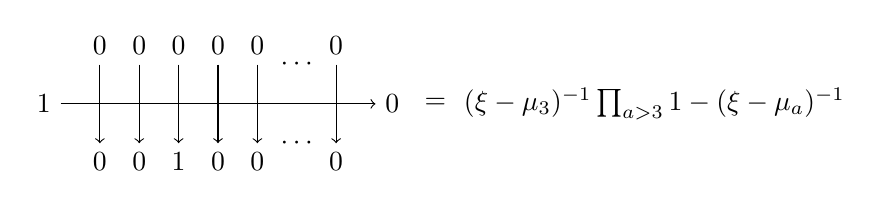
\begin{tikzpicture}
    \def\t{0.5}
    \def\s{-1.5}
    \def\k{1}
    \def\l{5}
    \def\ans{$(\xi-\mu_3)^{-1}\prod_{a > 3}\psquare{1-(\xi-\mu_a)^{-1}}$}
    \foreach \le/\ri/\y in {1/0/1} {
    \draw[->] (\s,\t-0.5*\y) node[anchor = east] {\le} -- ({\s+0.5*(\l+3)},\t-0.5*\y) node[anchor = west] {\ri};
    }
    \foreach \e/\x in {0/1,0/2,1/3,0/4,0/5,0/7} {
    \draw[->] ({\s+0.5*\x},\t) node[anchor = south] {$0$} -- ({\s+0.5*\x},{\t-0.5*(\k+1)}) node[anchor = north] {\e}  ;
    }
    \draw ({\s+0.5*(\l+1)},\t) node {$\cdots$};
    \draw ({\s+0.5*(\l+1)},{\t-0.5*(\k+1)}) node {$\cdots$};
    \draw ({\s+0.5*(\l+4)},{\t - 0.25*(\k+1)}) node[anchor = west] {=} ;
    \draw ({\s+0.5*(\l+5)},{\t - 0.25*(\k+1)}) node[anchor = west] {\ans};
    \end{tikzpicture}
\end{center}

Let us denote $\ket{a_1 a_2 \dots a_k}$ to be the state with $k$ 1s in the $a_1,a_2, \dots ,a_k$ positions. We can then rewrite 
\eq{
B(\xi)\Omega = \sum_{b\geq 1} (\xi - \mu_b)^{-1}\prod_{a > b}\psquare{1-(\xi-\mu_b)^{-1}} \ket{b}
}
We can then calculate the constituent terms in $A(\lambda)\ket{b}$ as 

\begin{center}
    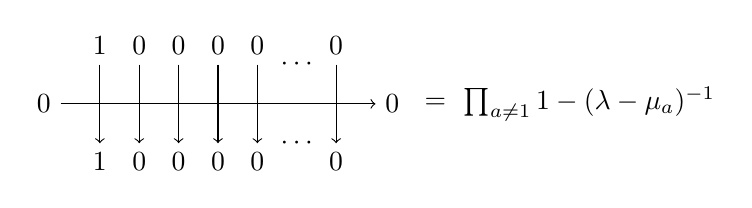
\begin{tikzpicture}
    \def\t{0.5}
    \def\s{-1.5}
    
    \def\k{1}
    \def\l{5}

    \def\ans{$\prod_{a \neq 1}\psquare{1-(\lambda-\mu_a)^{-1}}$}
    
    \foreach \le/\ri/\y in {0/0/1} {
    \draw[->] (\s,\t-0.5*\y) node[anchor = east] {\le} -- ({\s+0.5*(\l+3)},\t-0.5*\y) node[anchor = west] {\ri};
    }
    
    \foreach \u/\d/\x in {1/1/1,0/0/2,0/0/3,0/0/4,0/0/5,0/0/7} {
    \draw[->] ({\s+0.5*\x},\t) node[anchor = south] {\u} -- ({\s+0.5*\x},{\t-0.5*(\k+1)}) node[anchor = north] {\d}  ;
    }
    
    \draw ({\s+0.5*(\l+1)},\t) node {$\cdots$};
    \draw ({\s+0.5*(\l+1)},{\t-0.5*(\k+1)}) node {$\cdots$};
    
    \draw ({\s+0.5*(\l+4)},{\t - 0.25*(\k+1)}) node[anchor = west] {=} ;
    \draw ({\s+0.5*(\l+5)},{\t - 0.25*(\k+1)}) node[anchor = west] {\ans};
    \end{tikzpicture}
\end{center}

\begin{center}
    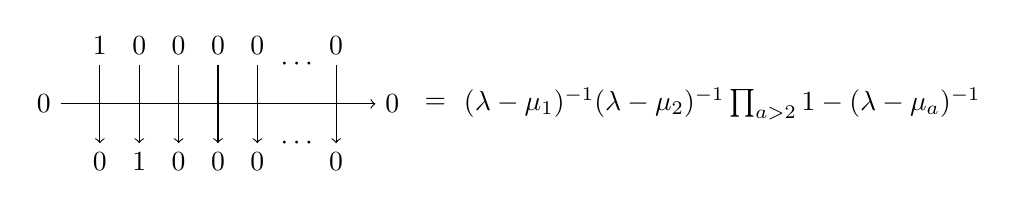
\begin{tikzpicture}
    \def\t{0.5}
    \def\s{-1.5}
    
    \def\k{1}
    \def\l{5}

    \def\ans{$(\lambda-\mu_1)^{-1}(\lambda-\mu_2)^{-1}\prod_{a>2}\psquare{1-(\lambda-\mu_a)^{-1}}$}
    
    \foreach \le/\ri/\y in {0/0/1} {
    \draw[->] (\s,\t-0.5*\y) node[anchor = east] {\le} -- ({\s+0.5*(\l+3)},\t-0.5*\y) node[anchor = west] {\ri};
    }
    
    \foreach \u/\d/\x in {1/0/1,0/1/2,0/0/3,0/0/4,0/0/5,0/0/7} {
    \draw[->] ({\s+0.5*\x},\t) node[anchor = south] {\u} -- ({\s+0.5*\x},{\t-0.5*(\k+1)}) node[anchor = north] {\d}  ;
    }
    
    \draw ({\s+0.5*(\l+1)},\t) node {$\cdots$};
    \draw ({\s+0.5*(\l+1)},{\t-0.5*(\k+1)}) node {$\cdots$};
    
    \draw ({\s+0.5*(\l+4)},{\t - 0.25*(\k+1)}) node[anchor = west] {=} ;
    \draw ({\s+0.5*(\l+5)},{\t - 0.25*(\k+1)}) node[anchor = west] {\ans};
    \end{tikzpicture}
\end{center}

\begin{center}
    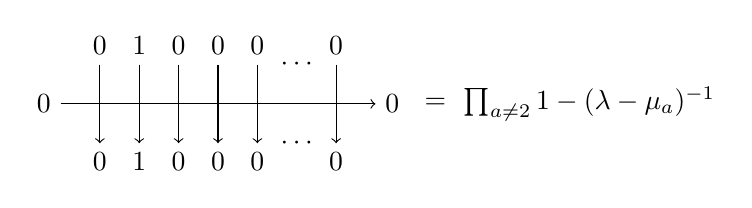
\begin{tikzpicture}
    \def\t{0.5}
    \def\s{-1.5}
    
    \def\k{1}
    \def\l{5}

    \def\ans{$\prod_{a\neq 2}\psquare{1-(\lambda-\mu_a)^{-1}}$}
    
    \foreach \le/\ri/\y in {0/0/1} {
    \draw[->] (\s,\t-0.5*\y) node[anchor = east] {\le} -- ({\s+0.5*(\l+3)},\t-0.5*\y) node[anchor = west] {\ri};
    }
    
    \foreach \u/\d/\x in {0/0/1,1/1/2,0/0/3,0/0/4,0/0/5,0/0/7} {
    \draw[->] ({\s+0.5*\x},\t) node[anchor = south] {\u} -- ({\s+0.5*\x},{\t-0.5*(\k+1)}) node[anchor = north] {\d}  ;
    }
    
    \draw ({\s+0.5*(\l+1)},\t) node {$\cdots$};
    \draw ({\s+0.5*(\l+1)},{\t-0.5*(\k+1)}) node {$\cdots$};
    
    \draw ({\s+0.5*(\l+4)},{\t - 0.25*(\k+1)}) node[anchor = west] {=} ;
    \draw ({\s+0.5*(\l+5)},{\t - 0.25*(\k+1)}) node[anchor = west] {\ans};
    \end{tikzpicture}
\end{center}

\begin{center}
    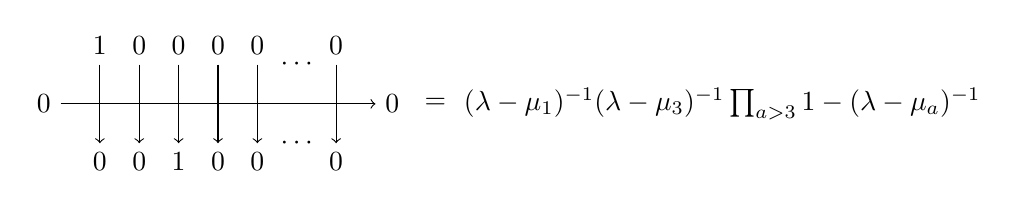
\begin{tikzpicture}
    \def\t{0.5}
    \def\s{-1.5}
    
    \def\k{1}
    \def\l{5}

    \def\ans{$(\lambda-\mu_1)^{-1}(\lambda-\mu_3)^{-1}\prod_{a>3}\psquare{1-(\lambda-\mu_a)^{-1}}$}
    
    \foreach \le/\ri/\y in {0/0/1} {
    \draw[->] (\s,\t-0.5*\y) node[anchor = east] {\le} -- ({\s+0.5*(\l+3)},\t-0.5*\y) node[anchor = west] {\ri};
    }
    
    \foreach \u/\d/\x in {1/0/1,0/0/2,0/1/3,0/0/4,0/0/5,0/0/7} {
    \draw[->] ({\s+0.5*\x},\t) node[anchor = south] {\u} -- ({\s+0.5*\x},{\t-0.5*(\k+1)}) node[anchor = north] {\d}  ;
    }
    
    \draw ({\s+0.5*(\l+1)},\t) node {$\cdots$};
    \draw ({\s+0.5*(\l+1)},{\t-0.5*(\k+1)}) node {$\cdots$};
    
    \draw ({\s+0.5*(\l+4)},{\t - 0.25*(\k+1)}) node[anchor = west] {=} ;
    \draw ({\s+0.5*(\l+5)},{\t - 0.25*(\k+1)}) node[anchor = west] {\ans};
    \end{tikzpicture}
\end{center}
In general, we see
\eq{
A(\lambda)\ket{b} &= 
\prod_{a \neq b} \psquare{1-(\lambda- \mu_a)^{-1}}
 \ket{b} + \sum_{c > b }(\lambda - \mu_b)^{-1} (\lambda - \mu_c)^{-1} \prod_{\substack{{a < b,} \\ {a > c}}} \psquare{1-(\lambda- \mu_a)^{-1}} \ket{c} \\
 %&= \prod_{a < b} \psquare{1 - (\lambda - \mu_a)^{-1}} \pbrace{\ket{b} + (\lambda-\mu_b)^{-1}\sum_{c > b}(\lambda - \mu_c)^{-1}\prod_{d > c} \psquare{1 - (\lambda - \mu_d)^{-1}}\ket{c}}
}
Note we always have that the $1$ is moving to the right. 
To continue to proceed let us now consider how $D$ acts on $B\Omega$: We see that terms in $D(\lambda)\ket{k}$ look like 

\begin{center}
    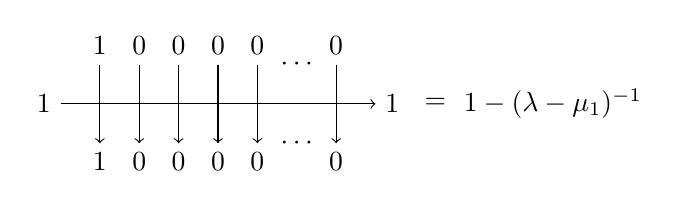
\begin{tikzpicture}
    \def\t{0.5}
    \def\s{-1.5}
    
    \def\k{1}
    \def\l{5}

    \def\ans{$\psquare{1-(\lambda-\mu_1)^{-1}}$}
    
    \foreach \le/\ri/\y in {1/1/1} {
    \draw[->] (\s,\t-0.5*\y) node[anchor = east] {\le} -- ({\s+0.5*(\l+3)},\t-0.5*\y) node[anchor = west] {\ri};
    }
    
    \foreach \u/\d/\x in {1/1/1,0/0/2,0/0/3,0/0/4,0/0/5,0/0/7} {
    \draw[->] ({\s+0.5*\x},\t) node[anchor = south] {\u} -- ({\s+0.5*\x},{\t-0.5*(\k+1)}) node[anchor = north] {\d}  ;
    }
    
    \draw ({\s+0.5*(\l+1)},\t) node {$\cdots$};
    \draw ({\s+0.5*(\l+1)},{\t-0.5*(\k+1)}) node {$\cdots$};
    
    \draw ({\s+0.5*(\l+4)},{\t - 0.25*(\k+1)}) node[anchor = west] {=} ;
    \draw ({\s+0.5*(\l+5)},{\t - 0.25*(\k+1)}) node[anchor = west] {\ans};
    \end{tikzpicture}
\end{center}

\begin{center}
    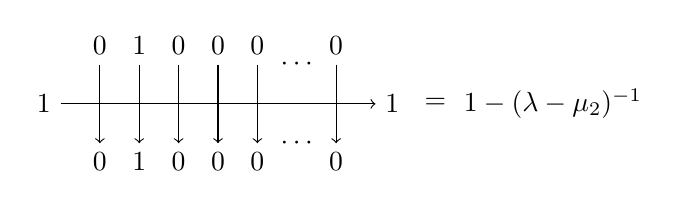
\begin{tikzpicture}
    \def\t{0.5}
    \def\s{-1.5}
    
    \def\k{1}
    \def\l{5}

    \def\ans{$\psquare{1-(\lambda-\mu_2)^{-1}}$}
    
    \foreach \le/\ri/\y in {1/1/1} {
    \draw[->] (\s,\t-0.5*\y) node[anchor = east] {\le} -- ({\s+0.5*(\l+3)},\t-0.5*\y) node[anchor = west] {\ri};
    }
    
    \foreach \u/\d/\x in {0/0/1,1/1/2,0/0/3,0/0/4,0/0/5,0/0/7} {
    \draw[->] ({\s+0.5*\x},\t) node[anchor = south] {\u} -- ({\s+0.5*\x},{\t-0.5*(\k+1)}) node[anchor = north] {\d}  ;
    }
    
    \draw ({\s+0.5*(\l+1)},\t) node {$\cdots$};
    \draw ({\s+0.5*(\l+1)},{\t-0.5*(\k+1)}) node {$\cdots$};
    
    \draw ({\s+0.5*(\l+4)},{\t - 0.25*(\k+1)}) node[anchor = west] {=} ;
    \draw ({\s+0.5*(\l+5)},{\t - 0.25*(\k+1)}) node[anchor = west] {\ans};
    \end{tikzpicture}
\end{center}

In general, we see 
\eq{
D(\lambda)\ket{b} = \psquare{1-(\lambda - \mu_b)^{-1}} \ket{b}
}
As such we get 
\eq{
\psquare{A(\lambda) + D(\lambda)}B(\xi)\Omega &= \sum_{b \geq 1} \psquare{A(\lambda) + D(\lambda)}  (\xi - \mu_b)^{-1}\prod_{a >b}\psquare{1-(\xi-\mu_a)^{-1}} \ket{b} \\
&= \sum_{b \geq 1}\left \lbrace (\xi - \mu_b)^{-1}\pround{\prod_{a > b}\psquare{1-(\xi-\mu_a)^{-1}}}\left[ \pround{\psquare{1-(\lambda - \mu_b)^{-1}} +  \prod_{a \neq b} \psquare{1 - (\lambda - \mu_a)^{-1}}}\ket{b} \right. \right. \\
&\phantom{=} \left. \left. + \sum_{c > b }(\lambda - \mu_b)^{-1} (\lambda - \mu_c)^{-1} \prod_{\substack{{a < b,} \\ {a > c}}} \psquare{1-(\lambda- \mu_a)^{-1}} \ket{c} \right] \right\rbrace \\
&= \sum_{b \geq 1}\left \lbrace (\xi - \mu_b)^{-1}\pround{\prod_{a > b}\psquare{1-(\xi-\mu_a)^{-1}}}\left( \psquare{1-(\lambda - \mu_b)^{-1}} +  \prod_{a \neq b} \psquare{1 - (\lambda - \mu_a)^{-1}} \right. \right. \\
&\phantom{=} \left. \left. + \sum_{c < b }(\lambda - \mu_b)^{-1} (\lambda - \mu_c)^{-1} \prod_{\substack{{a < c,} \\ {a > b}}} \psquare{1-(\lambda- \mu_a)^{-1}}  \right)\ket{b} \right\rbrace
}
Let us consider the multiplying term of $\ket{b}$
\eq{
\psquare{1-(\lambda - \mu_b)^{-1}} +  \prod_{a \neq b} \psquare{1 - (\lambda - \mu_a)^{-1}} + \sum_{c < b }(\lambda - \mu_b)^{-1} (\lambda - \mu_c)^{-1} \prod_{\substack{{a < c,} \\ {a > b}}} \psquare{1-(\lambda- \mu_a)^{-1}}
}

To complete the proof in the case $k=1$ we need that 
\eq{
\psquare{1-(\lambda - \mu_1)^{-1}} +  \prod_{a \neq 1} \psquare{1 - (\lambda - \mu_a)^{-1}} = \psquare{1-(\lambda - \xi)^{-1}} + \psquare{1+(\lambda - \xi)^{-1}}\prod_{a = 1}^n \psquare{1 - (\lambda - \mu_a)^{-1}} 
}
The condition we impose says 
\eq{
\prod_{a=1}^n \psquare{1 - (\xi - \mu_a)^{-1}} = 0 \Rightarrow \xi-\mu_b= 1 \quad \text{for some $b$} 
}
\hl{5: This doesn't look like it solves our problem}
\end{proof}

%%%%%%%%%%%%%%%%%%%%%%%%%%%%%%%%%%%%%
\subsection{The Heisenberg spin chain}
We may now convert our algebraic picture into physics: Let $\mc{R}(u) = uR(iu) = u + i P$. If we then let the transfer matrix be 
\eq{
\tau(u) = \tr_{\mbb{C}^2} \mc{R}_{0n}(u- \frac{i}{2}) \dots \mc{R}_{01}(u- \frac{i}{2}) 
}
We then define the Hamiltonian of the XXX-model to be 
\eq{
H_{XXX} = \ev{i \frac{d}{du}\log \tau(u)}{u=\frac{i}{2}}
}
and the shift operator to be 
\eq{
e^{iP} = i^{-n} \tau(\frac{i}{2})
}
Taking each $\mu_j = \frac{1}{2}$ we interpret the rep space of the evaluation module to be a quantum mechanic state space with each vector being a spin configuration of a chain of $n$ spin-$\frac{1}{2}$ states. \\
Now $H_{XXX}$ governs dynamics via Schrodinger's equation. As is typical in QM we want to look for stationary states, which are eigenstates of the Hamiltonian. We have already found these to be $v(\bm{\xi})$ using the Bethe ansatz. 

\begin{lemma}
The Hamiltonian $H_{XXX}$ can be explicitly computed as 
\eq{
H_{XXX} = \sum_{j=1^n} (\sigma_j^x\sigma_{j+1}^{x}+\sigma_j^y\sigma_{j+1}^{y}+\sigma_j^z\sigma_{j+1}^{z})
}
where $\sigma_j^x, \dots$ are the Pauli matrices. 
\end{lemma}


%%%%%%%%%%%%%%%%%%%%%%%%%%%%%%%%%%%%%
%%%%%%%%%%%%%%%%%%%%%%%%%%%%%%%%%%%%%
\section{Representation theory of quantum affine algebras}

%%%%%%%%%%%%%%%%%%%%%%%%%%%%%%%%%%%%%
\subsection{Introduction}
Let us work over $\mbb{C}$. Recall we define 
\eq{
\mf{sl}_2 = \pbrace{\begin{pmatrix}a & b \\ c & -a \end{pmatrix} \, | \, a,b,c \in \mbb{C}}
}
This algebra has a standard basis given by 
\eq{
e &= \begin{pmatrix}0 & 1 \\ 0 & 0 \end{pmatrix} \\
f &= \begin{pmatrix}0 & 0 \\ 1 & 0 \end{pmatrix} \\
h &= \begin{pmatrix}1 & 0 \\ 0 & -1 \end{pmatrix}
}
and these have commutation relations 
\eq{
\comm[e]{f} &= h \\
\comm[h]{e} &= 2e \\
\comm[h]{f} &= -2f
}
We then make a new definition of $\mf{sl}_2$ simply as the Lie algebra generated by $e,f,h$ with the above commutation relations. We can then study $\mf{sl}_2$ representations, i.e. LA homs $\mf{sl}_2 \to \End(V)$ for some vector space $V$ with the bracket on the RHS being commutation. We have some natural reps;
\begin{itemize}
    \item Fundamental rep with $V = \mbb{C}^2$, and sending $e \mapsto \begin{psmallmatrix} 0 & 1 \\ 0 & 0 \end{psmallmatrix} $, etc. 
    \item Adjoint rep with $V = \mbb{C}^3$, sending $e \mapsto \begin{psmallmatrix} 0 & 2 & 0 \\ 0 & 0 & 1 \\ 0 & 0 & 0 \end{psmallmatrix}$, etc. 
\end{itemize}

For any LA $\mf{g}$ we have the Universla enveloping algebra $U(\mf{g}) = \faktor{T(\mf{g})}{I}$ where $I = \pangle{x \otimes y - y \otimes x - \comm[x]{y}}$ is an ideal. We get a natural embedding $i:\mf{g} \hookrightarrow U(\mf{g})$. The pair $(U(\mf{g}),i)$ has the universal property: 
\begin{tkz}
U(\mf{g}) \arrow[dr,dashed, "\exists ! \bar{\phi}"] & \\
\mf{g} \arrow[u,"i"] \arrow[r,"\phi"'] & A 
\end{tkz}
for an associative algebra hom $\phi: \mf{g} \to A$. 

\begin{idea}
$U(\mf{g})$ contains all the information of reps of $\mf{g}$
\end{idea}

\begin{example}
$U(\mf{sl}_2)$ is the unital associative algebra  defined by $e,f,h$ with the commutation relations. 
\end{example}

\begin{prop}
$U(\mf{g})$ is a co-commutative Hopf algebra with co-product 
\eq{
\Delta : U(\mf{g}) &\to U(\mf{g}) \otimes U(\mf{g}) \\
\mf{g} \ni x &\mapsto 1 \otimes x + x \otimes 1  
}
and counit $\eps(x) = 0$, antipode $S(x) = -x$.
\end{prop}

Now we want to deform the Hopf algebra structure to get a non-commutative Hopf algebra that is now quasi-triangular (braided) 

%%%%%%%%%%%%%%%%%%%%%%%%%%%%%%%
\subsection{The Hopf algebra \secmath{U_q(\mf{sl}_2)}}

Let $q \in \mbb{C}\setminus \pbrace{-1,0,1}$. 

\begin{definition}
$U_q(\mf{sl}_2)$ is the unital associative $\mbb{C}$-algebra
on the generators $e,f, t^{\pm 1}$ with relations 
\eq{
t e t^{-1} &= q^2 e \\
t f t^{-1} &= q^{-2} f \\
tt^{-1} &= 1 = t^{-1}t \\
\comm[e]{f} &= \frac{t - t^{-1}}{q - q^{-1}}
}
If we consider the limit $q \to 1$ we should recover $U(\mf{sl}_2)$.
\end{definition}

\begin{ex}
Justify the relations of $U_q(\mf{g})$ by 
\begin{enumerate}
    \item Formally setting $t = q^h$
    \item Let $q \to 1$
    \item Recover $U(\mf{sl}_2)$
\end{enumerate}
For example, consider the relation $t e t^{-1} = q^2 e$. In $U(\mf{sl}_2)$ the relation is $\comm[h]{e} = 2e \Rightarrow he =e(h+2)$. Now 
\begin{enumerate}
    \item Let $t = q^h = \sum_{m \geq 0} \frac{1}{m!} (\log q)^m h^m$. Then 
    \eq{
    te &=  \sum_{m \geq 0} \frac{1}{m!} (\log q)^m h^m e\\
    &=  \sum_{m \geq 0} \frac{1}{m!} (\log q)^m e(h+2)^m \\
    &= \dots \\
    &= q^2 et
    }
\end{enumerate}
\end{ex}

We can give $U_q(\mf{sl}_2)$ a Hopf algebra structure by having 
\eq{
\Delta(e) &= e \otimes 1 +t \otimes e \\
\Delta(f) &= f \otimes t^{-1} + 1 \otimes f \\
\Delta(t^{\pm 1}) &= t^{\pm 1} \otimes t^{\pm 1} \\
\eps(e) &= 0 = \eps(f) \\
\eps(t^{\pm 1}) &= 1 \\
S(e) &= -t^{-1} e \\
S(f) &= - ft \\
S(t^{\pm 1}) &= t^{\mp}
}

\begin{ex}
Show that $\Delta, \eps, S$ preserve algebra relations. For example we have 
\eq{
S(ef - fe - \frac{t - t^{-1}}{q - q^{-1}}) &= S(f) S(e) - S(e) S(f) - \frac{S(t) - S(t^{-1})}{q -q^{-1}} \\
&= (-ft)(-t^{-1}e) - (-t^{-1}e)(-ft) - \frac{t - t^{-1}}{q - q^{-1}} \\
&= ef - fe - \frac{t - t^{-1}}{q - q^{-1}} = 0
}
\end{ex}


%%%%%%%%%%%%%%%%%%%%%%%%%%%%%%%%%%%%%%%%%%%%%%%
\subsection{\secmath{\text{Irreps of $U_q(\mf{sl}_2)$}}}

\begin{definition}
Choose a basis $v_0,v_1$ of $\mbb{C}^2$ and wrt this basis define 
\eq{
\pi(e) &= \begin{pmatrix}0 & 1 \\ 0 & 0 \end{pmatrix} \\
\pi(f) &= \begin{pmatrix}0 & 0 \\ 1 & 0 \end{pmatrix} \\
\pi(t) &= \begin{pmatrix}q & 0 \\ 0 & q^{-1} \end{pmatrix} = q^{\begin{psmallmatrix} 1 & 0 \\ 0 & -1\end{psmallmatrix} }
}
i.e. $\pi(e)(v_1) = v_0, \, \pi(f)(v_0) = v_1, \, \pi(t)(v_0) = qv_0, \, \pi(t)(v_1) = q^{-1}v_1$. The linear map $\pi:U_q(\mf{sl}_2) \to \End(\mbb{C}^2)$ is called the \bam{vector rep} of $U_q(\mf{sl}_2)$
\end{definition}

\begin{ex}
Check that $\pi$ is a LA hom. E.g. 
\eq{
\pi\pround{\frac{t-t^{-1}}{q-q^{-1}}} &= \frac{\pi(t) - \pi(t)^{-1}}{q-q^{-1}} = \frac{1}{q-q^{-1}}\psquare{\begin{pmatrix}q & 0 \\ 0 & q^{-1} \end{pmatrix} - \begin{pmatrix}q^{-1} & 0 \\ 0 & q \end{pmatrix}} = \begin{pmatrix} 1 & 0 \\ 0 & -1 \end{pmatrix} \\
\pi(\comm[e]{f}) &= \pi(e) \pi(f) - \pi(f) \pi(e) =  \begin{pmatrix}0 & 1 \\ 0 & 0 \end{pmatrix}\begin{pmatrix}0 & 0 \\ 1 & 0 \end{pmatrix} -  \begin{pmatrix}0 & 0 \\ 1 & 0 \end{pmatrix}\begin{pmatrix}0 & 1 \\ 0 & 0 \end{pmatrix} = \begin{pmatrix} 1 & 0 \\ 0 & -1 \end{pmatrix}
}
\end{ex}

\begin{definition}
We let 
\eq{
[n] = \frac{q^n - q^{-n}}{q - q^{-1}} = q^{n-1} + q^{n-3} + \dots + q^{3-n} + q^{1-n}
}
and call it a \bam{q-integer}
\end{definition}

\begin{lemma}
The q-integers obey 
\begin{itemize}
    \item $[1] = 1$
    \item $\lim_{q \to 1}[n] = n$
\end{itemize}
\end{lemma}

\begin{definition}
Let $V^{(n)} = \mbb{C} v_0^{(n)} \oplus \dots \oplus \mbb{C}v_n^{(n)}$ for $n \geq 0$. Note $\dim V^{(n)} = n+1$. Set 
\eq{
\pi^{(n)}(e)(v_i^{(n)}) &= [n-i+1] v_{i-1}^{(n)} \\
\pi^{(n)}(f )(v_i^{(n)}) &= [i+1] v_{i+1}^{(n)} \\
\pi^{(n)}(t)(v_i^{(n)}) &= q^{n-2i} v_{i}^{(n)}
}
where $v_{-1}^{(n)} = 0 = v_{n+1}^{(n)}$. This is called the \bam{Spin}-$\mathbf{\frac{n}{2}}$ rep of $U_q(\mf{sl}_2)$. 
\end{definition}

\begin{remark}
Considering the $n=0$ example, we get $V^{(0)} \cong \mbb{C}$, and 
\eq{
\pi^{(0)}(e) v_0^{(0)} &= 0 = \pi^{(0)}(f) v_0^{(0)} \\
\pi^{(0)}(t) v_0^{(0)} &= v_0^{(0)}
}
i.e. we have the trivial rep. We also can see $\pi^{(1)} = \pi$. 
\end{remark}

%%%%%%%%%%%%%%%%%%%%%%%%%%%%%%%%%%%%%%%%%%
\subsection{\secmath{\text{Tensor products of $U_q(\mf{sl}_2)$ reps}}}

\begin{idea}
It turns out we want a counit to have trivial reps, antipodes to have dual reps, and coproducts in order to have tensor products of reps. 
\end{idea}

Use the coproduct as follows: 
\eq{
((\pi_1,V_1),(\pi_2,V_2)) &\mapsto (\pi_{12},V_1 \otimes V_2)
}
where we take 
\eq{
\pi_{12}(x) = (\pi_1 \otimes \pi_2)(\Delta(x)) \in \End(V_1) \otimes \End(V_2) \cong \End(V_1 \otimes V_2)
}

\begin{theorem}
$\forall n,m \in \mbb{Z}_{\geq 0}$ we have 
\eq{
V^{(n)} \otimes V^{(m)} \cong V^{(n+m)} \oplus V^{(n+m-2)} \oplus \dots \oplus V^{(\abs{n-m})}
}
as $U_q(\mf{sl}_2)$-modules
\end{theorem}

\begin{example}
Take $n=m=1$ so $V^{(1)} \otimes V^{(1)} \cong V^{(2)} \oplus V^{(0)}$. Letting $u_0 = v_0^{(1)} \otimes v_0^{(1)}$ we have   
\eq{
e \cdot u_0 &=  \Delta(e)(v_0^{(1)} \otimes v_0^{(1)}) = (e \otimes 1 + t \otimes e)(v_0^{(1)} \otimes v_0^{(1)})  = 0 \\
[1]u_1 = f \cdot u_0 &=(f \otimes t^{-1} + 1 \otimes f)(v_0^{(1)} \otimes v_0^{(1)}) = q^{-1}v_1^{(1)} \otimes v_0^{(1)} + v_0^{(1)} \otimes v_1^{(1)} \\
[2]u_2 = f \cdot u_1 &=(f \otimes t^{-1} + 1 \otimes f)(q^{-1}v_1^{(1)} \otimes v_0^{(1)} + v_0^{(1)} \otimes v_1^{(1)})= (q+q^{-1})v_1^{(1)} \otimes v_1^{(1)} \\
f \cdot u_2 &= 0
}
Hence $W^{(2)} = \mbb{C} u_0 \oplus \mbb{C} u_1 \oplus \mbb{C} u_2$ is a submodule. We have 
\eq{
W^{(2)} &\overset{\cong}{\to} V^{(2)} \\
u_i &\mapsto v_i^{(2)}
}
If we let $\tilde{u} = q v_1^{(1)} \otimes v_0^{(1)} - v_0^{(1)} \otimes v_1^{(1)}$ we find $e \cdot \tilde{u} = 0 = f \cdot \tilde{u}, \, t \cdot \tilde{u} = \tilde{u}$, and so we have the submodule $W^{(0)} = \mbb{C} \tilde{u} \cong V^{(0)}$. Hence we have found 
\eq{
V^{(1)} \otimes V^{(1)} = W^{(2)} \oplus W^{(0)} \cong V^{(2)} \oplus V^{(0)}
}
as the theorem states. As $q \to 1$, $W^{(2)}$ are symmetric tensors in $V^{(1)} \oplus V^{(1)}$ and $W^{(0)}$ are antisymmetric. 
\end{example}

%%%%%%%%%%%%%%%%%%%%%%%%%%%%%%%%%%%%%%%%%%
\subsection{\secmath{U_q(\hat{\mf{sl}_2})}}

We now need to introduce another quantum parameter, so we will take $z$, the \bam{loop parameter}, which will be related to the spectral parameter $u$ by $z = e^{2u}$. \\
We will follow work by Drinfeld and Jimbo: deform the UEA of a Kac-Moody Lie algebra. Kac-Moody algebras include all finite-dimensional semi-simple Lie algebras through the Chevally-Serre presentation, but that also include loop algebras of the semi-simple LAs. This information can be represented in terms of Dynkin diagrams, or equivalently Cartan matrices. \\

\begin{definition}
$U_q(\hat{\mf{sl}_2})$ is the unital associative algebra on the generators $e_i,f_i, t_i^{\pm 1}$, $i =0,1$ with 
\eq{
t_i e_j t_i^{-1} &= q^{a_{ij}} e_j \\
t_i f_j t_i^{-1} &= q^{-a_{ij}} f_j \\
\comm[e_i]{f_j} &= \delta_{ij}\frac{t_i - t_i^{-1}}{q-q^{-1}} \\
t_i t_i^{-1} &= 1 =t_i^{-1} t_i \\
t_i t_j &= t_j t_i \\
e_i e_j^3 - [3] e_j e_i e_j^2 + [3] e_j^2 e_i e_j - e_j^3 e_i &= 0 \quad \text{(the $\mathbf{q}$\textbf{-Serre relations}, also exists for f)} 
}
Here $a = \begin{psmallmatrix} 2 & -2 \\ -2 & 2 \end{psmallmatrix}$ is the Cartan matrix. The is called the \bam{Chevalley generator realisation}.
\end{definition}

\begin{remark}
The definition for the q-deformed UEA for a different Kac-Moody algebra behaves the same using its corresponding Cartan matrix.
\end{remark}

\begin{prop}
We can make $U_q(\hat{\mf{sl}_2})$ into a Hopf algebra with 
\eq{
\Delta(e_i) &= e_i \otimes 1 + t_i \otimes e_i \\
\Delta(f_i) &= f_i \otimes t_i^{-1} + 1 \otimes f_i \\
\Delta(t_i) &= t_i \otimes t_i \\
\eps(e_i) &= 0 \\
\eps(f_i) &= 0 \\
\eps(t_i) &= 1 \\
S(e_i) &= - t_i^{-1} e_i \\
S(f_i) &= -f_i t_i \\
S(t_i) &= t_i^{-1}
}
\end{prop}

\begin{definition}
Given a Lie algebra $\mf{g}$ we can define 
\begin{itemize}
    \item The loops algebra $L\mf{g} = \mf{g} \otimes C^\infty(S^1) = \mf{g} \otimes \mbb{C}[z,z^{-1}] $
    \item The affine Lie algebra $\hat{\mf{g}} = L\mf{g} \oplus \mbb{C}c$
    \item The extended affine Lie algebra $\tilde{\mf{g}} = \hat{\mf{g}} + \mbb{C}d$. 
\end{itemize}
\end{definition}

%%%%%%%%%%%%%%%%%%%%%%%%%%%%%%%%%%%
\subsection{Evaluation reps of \secmath{U_q(\hat{\mf{sl}_2})}}

\begin{lemma}
Let $z \in \mbb{C}^\times$ be spectral parameter. Then $\exists ev_z: U_q(\hat{\mf{sl}_2}) \to U_q(\mf{sl}_2)$ a LA hom s.t. 
\eq{
ev_z(e_0) &= zf \\
ev_z(f_0) &= z^{-1}e \\
ev_z(t_0) &= t^{-1} \\ \\
ev_z(e_1) &= e \\
ev_z(f_1) &= f \\
ev_z(t_1) &= t
}
\end{lemma}
\begin{ex}
Check that the relations of $U_q(\hat{\mf{sl}_2})$ are preserved. E.g. 
\eq{
ev_z\pround{\comm[e_0]{f_0} - \frac{t_0 - t_0^{-1}}{q - q^{-1}}} &= \comm[zf]{z^{-1}e} - \frac{t^{-1} - t}{q - q^{-1}} \\
&= \comm[f]{e} + \frac{t - t^{-1}}{q - q^{-1}} = 0 
}
\end{ex}


This means we can now get the diagram 
\begin{tkz}
U_q(\hat{\mf{sl}_2}) \arrow[r,"ev_z"] \arrow[dr,"\pi_z^{(n)}"']& U_q(\mf{sl}_2)  \arrow[d,"\pi^{(n)}"] \\
& \End(V^{(n)})
\end{tkz}
In this representation we call the rep space $V_z^{(n)}$.

\begin{example}
When $n=1$ the rep space is $V^{(1)}_z\cong \mbb{C}^2$, and the rep $\pi_z^{(1)}$ is 
\eq{
\pi_z^{(1)}(e_0) &= \begin{pmatrix} 0 & 0 \\ z & 0\end{pmatrix} = z \pi_z^{(1)}(f_1)\\ 
\pi_z^{(1)}(f_0) &= \begin{pmatrix} 0 & z^{-1} \\ 0 & 0\end{pmatrix} = z^{-1} \pi_z^{(1)}(e_1) \\ 
\pi_z^{(1)}(t_0) &= \begin{pmatrix} q & 0 \\ 0 & q^{-1}\end{pmatrix} = \pround{\pi_z^{(1)}(t_1)}^{-1} 
}
\end{example}

%%%%%%%%%%%%%%%%%%%%%%%%%%%%%%%%%%%%%%
\subsection{Tensor products}

\begin{theorem}
$V_{z_1}^{(1)} \otimes V_{z_2}^{(1)}$ is irreducible as a $U_q(\hat{\mf{sl}_2})$-module iff $z_1 \neq z_2 q^{\pm 2}$. Otherwise we get two SESs
\begin{tkz}
(i) & 0 \arrow[r] & V_z^{(2)} \arrow[r,"i"] & V_{zq^{-1}}^{(1)} \otimes V_{zq}^{(1)} \arrow[r,"\tau"] & V_z^{(0)} \arrow[r] & 0 \\
(ii) & 0 \arrow[r] & V_z^{(0)} \arrow[r,"i^\prime"] & V_{zq}^{(1)} \otimes V_{zq^{-1}}^{(1)} \arrow[r,"\tau^\prime"] & V_z^{(2)} \arrow[r] & 0 
\end{tkz}
\end{theorem}
\begin{proof}
\hl{$(i)$ is an exercise:} \\
For the second sequence, consider $w = v_0 \otimes v_1 - q v_1 \otimes v_0 \in V_{z_1}^{(1)} \otimes V_{z_2}^{(1)}$. We may calculate
\eq{
(\pi_{z_1}^{(1)} \otimes \pi_{z_2}^{(1)}) (\Delta(e_1))(w) &= (\pi_{z_1}^{(1)} \otimes \pi_{z_2}^{(1)})(e_1 \otimes 1 + t_1 \otimes e_1)(v_0 \otimes v_1 - q v_1 \otimes v_0) \\
&= (\pi_{z_1}^{(1)}(e_1) \otimes 1 + \pi_{z_1}^{(1)}(t_1) \otimes \pi_{z_2}^{(1)}(e_1))(v_0 \otimes v_1 - q v_1 \otimes v_0) \\
&= -q v_0 \otimes v_0 + q^{-1}q v_0 \otimes v_0 = 0 
}
It can also be shown 
\eq{
(\pi_{z_1} \otimes \pi_{z_2}) (\Delta(f_1))(w) &= 0
}
Hence $\mbb{C}w$ is a 1-dimensional submodule of $U_q(\mf{sl}_2)$. However 
\eq{
(\pi_{z_1} \otimes \pi_{z_2}) (\Delta(e_0))(w) &= (z_1 - q^2 z_2) v_1 \otimes v_1
}
and so this is 0 iff $z_1 = z_2 q^2$, meaning we get a $U_q(\hat{\mf{sl}}_2)$ iff $z_1 = z_2 q^2$ . \\
\hl{To finish this proof, use example on tensor product of reps as direct sums}. 
\end{proof}

\begin{remark}
The SES $(i)$ tells us that $V_z^{(2)} \hookrightarrow V_{zq^{-1}}^{(1)} \otimes V_{zq}^{(1)}$ is an embedding, and that 
\eq{
\faktor{V_{zq^{-1}}^{(1)} \otimes V_{zq}^{(1)}}{\image(\tau)} \cong V_z^{(0)}
}
\end{remark}

\hl{Now we do know that $V_{zq^{-1}}^{(1)} \otimes V_{zq}^{(1)} \cong V_z^{(2)} \oplus V_z^{(0)}$ as vector spaces from the above.(Had this copied down from lectures, but think this is incorrect now - think about it)}  

%%%%%%%%%%%%%%%%%%%%%%%%%%%%%%%%%%%%
\subsection{R-matrices}

We have seen that if $z_i$ are generic then we have $V_{z_1}^{(1)} \otimes V_{z_2}^{(2)}$, $V_{z_2}^{(1)} \otimes V_{z_1}^{(2)}$ are irreducible as $U_q(\hat{\mf{sl}_2})$-modules. \\
We will see they are isomorphic as the modules, as it turns out $\exists \check{R}(z_1, z_2) : V_{z_1}^{(1)} \otimes V_{z_2}^{(2)} \to V_{z_2}^{(1)} \otimes V_{z_1}^{(2)}$ invertible s.t. 
\eq{
\check{R}(z_1, z_2)(\pi_{z_1} \otimes \pi_{z_2})(\Delta(x)) = (\pi_{z_2} \otimes \pi_{z_1})(\Delta(x)) \check{R}(z_1, z_2)
}

\begin{lemma}[Schur's lemma]
If $A$ is a $\mbb{C}$-algebra and $V, W$ are irreps of $A$, then if $\exists \phi_1, \phi_2 : V \to W$ non-zero homomorphisms of $A$-modules then 
\begin{enumerate}
    \item these are isomorphisms
    \item If $V=W$, then $\exists \lambda_i \in \mbb{C}$ s.t. $\phi_i = \lambda_i \id$
    \item $\exists \lambda \in \mbb{C}$ s.t. $\phi_1 = \lambda \phi_2$
\end{enumerate}
\end{lemma}
\begin{proof}
$1)$ First note that $\ker \phi_i, \image \phi_i $ are submodules of $V,W$ respectively as 
\eq{
\forall v \in \ker\phi_i, \, z \in \mbb{C}, \, \phi_i(z \cdot v) = z \cdot \phi_i(v) = 0 &\Rightarrow z \cdot v \in \ker\phi_i \\
\forall w=\phi_i(u) \in \image\phi_i, \, z \in \mbb{C}, \, z\cdot w = \phi_i(z \cdot u) &\Rightarrow z\cdot w \in \image \phi_i 
}
They are also clearly closed under addition. Then as neither $V,W$ have non-trivial proper submodules, and $\phi_i \neq 0$, we must have $\ker\phi_i = 0, \, \image \phi_i = W \Rightarrow \phi_i$ is an iso. \\
$2)$ We know $\phi_i$ must have an eigenvalue \hl{(I know this to be true for f.d. vector spaces by fundamental theorem of algebra, why in general?)} $\lambda_i$. Then the map 
\eq{
\phi_i -\lambda_i \id : W \to W
}
must have a non-zero kernel, which by irreducibility we know must be all of $V$, hence $\phi_i = \lambda_i \id$. \\
$3)$ Consider $\phi_1 \circ \phi_2^{-1} : W \to W$. by $2)$ there must be $\lambda \in \mbb{C}$ s.t. $\phi_1 \circ \phi_2^{-1} = \lambda \id \Rightarrow \phi_1 = \lambda \phi_2$. 
\end{proof}

\begin{prop}
$\exists ! \, \check{R}$ satisfying the required condition normalised s.t. 
\eq{
\check{R}(z_1, z_2) (v_0^{(1)} \otimes v_0^{(1)}) = v_0^{(1)} \otimes v_0^{(1)}
}
\end{prop}
\begin{proof}
Uniqueness comes from Schur's lemma, and the answer is explicitly 
\eq{
\check{R}(z_1, z_2) = \begin{pmatrix} 1 & 0 & 0 & 0 \\
0 & \frac{z_1(q-q^{-1})}{z_1 q - z_2 q^{-1}} & \frac{z_1 - z_2}{z_1 q - z_2 q^{-1}} & 0 \\
0 & \frac{z_1 - z_2}{z_1 q - z_2 q^{-1}} & \frac{z_2(q-q^{-1})}{z_1 q - z_2 q^{-1}} & 0 \\
0 & 0 & 0 & 1
\end{pmatrix}
}
\end{proof}

We can then define an $R$-matrix by $R = P\check{R} : V_{z_1}^{(1)} \otimes V_{z_2}^{(1)} \to V_{z_1}^{(1)} \otimes V_{z_2}^{(1)}$, where recall $P(v \otimes w) = w \otimes v$.  

\begin{prop}
$R(z_1, z_2) \Delta(x) = \Delta^\prime R(z_1, z_2)$, where $\Delta^\prime = P \Delta P$ is the opposite ordered coproduct. 
\end{prop}

\begin{remark}
Note $\check{R}(z_1,z_2) = \check{R}\pround{\frac{z_1}{z_2}}$, and hence so is $R$. 
\end{remark}

%%%%%%%%%%%%%%%%%%%%%%%%%%%%%%%%%%%%%%%%%%%%%%%%%%%%%%%%
\subsection{The Yang-Baxter equation}
Noting that $V_{z_1}^{(1)} \otimes V_{z_2}^{(1)} \otimes V_{z_3}^{(1)}$ is generically irreducible, we can construct an isomorphism to $V_{z_3}^{(1)} \otimes V_{z_2}^{(1)} \otimes V_{z_1}^{(1)}$ in two ways: 

\begin{center}
    \begin{tikzpicture}[commutative diagrams/every diagram]
\node (P0) at (90:2.6cm) {$V_{z_1}^{(1)} \otimes V_{z_2}^{(1)} \otimes V_{z_3}^{(1)}$};
\node (P1) at (90+60:2.3cm) {$V_{z_2}^{(1)} \otimes V_{z_1}^{(1)} \otimes V_{z_3}^{(1)}$} ;
\node (P2) at (90+2*60:2.3cm) {$V_{z_2}^{(1)} \otimes V_{z_3}^{(1)} \otimes V_{z_1}^{(1)}$};
\node (P3) at (90+3*60:2.6cm) {$V_{z_3}^{(1)} \otimes V_{z_2}^{(1)} \otimes V_{z_1}^{(1)}$};
\node (P4) at (90+4*60:2.3cm) {$V_{z_1}^{(1)} \otimes V_{z_3}^{(1)} \otimes V_{z_2}^{(1)}$};
\node (P5) at (90+5*60:2.3cm) {$V_{z_3}^{(1)} \otimes V_{z_1}^{(1)} \otimes V_{z_2}^{(1)}$};

\path[commutative diagrams/.cd, every arrow, every label]
(P0) edge node[swap] {$\check{R}(z_1,z_2) \otimes 1$} (P1)
(P1) edge node[swap] {$1 \otimes \check{R}(z_1,z_3)$} (P2)
(P2) edge node[swap] {$\check{R}(z_2,z_3) \otimes 1$} (P3)
(P0) edge node {$1 \otimes \check{R}(z_2,z_3)$} (P5)
(P5) edge node {$\check{R}(z_1,z_3) \otimes 1$} (P4)
(P4) edge node {$1 \otimes \check{R}(z_1,z_2)$} (P3) ;
\end{tikzpicture}
\end{center}

by Schur's lemma, they are proportional, and computing the action on $v_0 \otimes v_0 \otimes v_0$, they are equal, and we find 
\eq{
\psquare{\check{R}(z_2,z_3) \otimes 1} \psquare{1 \otimes \check{R}(z_1,z_3)} \psquare{\check{R}(z_1,z_2) \otimes 1} = \psquare{1 \otimes \check{R}(z_1,z_2)}\psquare{\check{R}(z_1,z_3) \otimes 1}\psquare{1 \otimes \check{R}(z_2,z_3)}
}
this is the \bam{Yang-Baxter equation (YBE)} or the \bam{braid relation}. In terms of $R$ this becomes the standard CYBE. 

%%%%%%%%%%%%%%%%%%%%%%%%%%%%%%%%%%%%%%%%%%%%%%%%%%%%%%%%
\subsection{The Universal R-matrix}
So far we have discussed Hopf algebras $U$ with coproduct $\Delta$, counit $\eps$, and antipode $S$. Now consider a Hopf algebra equipped with some extra structure 

\begin{definition}
A \bam{universal R matrix} is $\mc{R} \in U \otimes U$ that satisfies 
\begin{enumerate}
    \item $\mc{R}\Delta = \Delta^\prime \mc{R}$
    \item $(\Delta \otimes 1)\mc{R} = \mc{R}_{13} \mc{R}_{23}$
    \item $(1 \otimes \Delta)\mc{R} = \mc{R}_{13} \mc{R}_{12}$
\end{enumerate}
\end{definition}

\begin{prop}
$\mc{R}$ satisfies the algebraic YBE in $U \otimes U \otimes U$
\eq{
\mc{R}_{23} \mc{R}_{13} \mc{R}_{12} = \mc{R}_{12} \mc{R}_{13} \mc{R}_{23}
}
\end{prop}
\begin{proof}
Use the notation $R = \sum_i A_i \otimes B_i$. Then the LHS is 
\eq{
\mc{R}_{23} (1 \otimes \Delta)\mc{R} &= \mc{R}_{23} \psquare{\sum_i A_i \otimes \Delta(B_i)} \\
&= \psquare{\sum_i A_i \otimes \Delta^\prime(B_i)} \mc{R}_{23} \\
&= P_{23} \psquare{\sum_i A_i \otimes \Delta(B_i)} P_{23} \mc{R}_{23} \\
&= P_{23} \mc{R}_{13} \mc{R}_{12} P_{23} \mc{R}_{23} = \mc{R}_{12} \mc{R}_{13} \mc{R}_{23}
}
\end{proof}

\begin{theorem}
It is possible to construct such an $\mc{R}$ for $U_q(\mf{g})$, and $\mc{R}$ lies in an extension of $U_q(\mf{g}) \otimes U_q(\mf{g})$. 
\end{theorem}

Given reps $(\pi_V,V), (\pi_W,W)$, we can construct $\mc{R}_{VW}  : V \otimes W \to V \otimes W $ by 
\eq{
\mc{R}_{VW} = (\pi_V \otimes \pi_W) \mc{R}
}
\begin{prop}
$\mc{R}_{VW}$ satisfies 
\begin{enumerate}
    \item $\mc{R}_{VW}(\pi_V \otimes \pi_W) \Delta = (\pi_V \otimes \pi_W) \Delta^\prime \mc{R}_{VW}$
    \item $\mc{R}_{V_1 \otimes V_2,W} = \mc{R}_{V_1 ,W}\mc{R}_{V_2,W}$
    \item $\mc{R}_{V,W_1 \otimes W_2} = \mc{R}_{V,W_1} \mc{R}_{V,W_2}$
    \item $\mc{R}_{V_1,V_2}\mc{R}_{V_1,V_3} \mc{R}_{V_2,V_3} = \mc{R}_{V_2,V_3} \mc{R}_{V_1,V_3} \mc{R}_{V_1,V_2}$
\end{enumerate}
\end{prop}

\begin{example}
$R(z_1,z_2) = \mc{R}_{V_{z_1}^{(1)},V_{z_2}^{(1)}} = (\pi_{V_{z_1}^{(1)}} \otimes \pi_{V_{z_2}^{(1)}})\mc{R}$
\end{example}

%%%%%%%%%%%%%%%%%%%%%%%%%%%%%%%%%%%%%%%%%%%%%%%%%%%%%%%%
\subsection{The RTT relation}

\begin{remark}
Note that letting $z = q^{-2u}, q = e^{\eta}$, we get 
\eq{
R(z) = \begin{pmatrix} \sinh(\eta(1-u)) & 0 & 0 & 0 \\
0 & \sinh(-\eta u) & e^{\eta u}\sinh(\eta) & 0 \\
0 & e^{\eta u}\sinh(\eta) & \sinh(-\eta u) & 0 \\
0 & 0 & 0 & \sinh(\eta(1-u)) 
\end{pmatrix} = -u\eta (1-u^{-1}P) + \mc{O}(\eta^2)
}
Hence we can view our $R(z)$ as a deformation of Yang's R-matrix. As such we can repeat the approach of defining Hopf algebra structure from an R-matrix, with out new matrix. \\
The two approaches can be seen symbolically as the following: 
\eq{
R(u) &\to \text{Hopf algebra} \\
\text{Hopf algebra} + \mc{R} &\to R(z)
}
It is a natural question to ask whether these Hopf algebras are the same, and it is a theorem of Reshetikhin and Semenov-Tian-Shansky that they are. 
\end{remark}

%%%%%%%%%%%%%%%%%%%%%%%%%%%%%%%%%%%%%%%%%%%%%%%%%%%%%%%%
%%%%%%%%%%%%%%%%%%%%%%%%%%%%%%%%%%%%%%%%%%%%%%%%%%%%%%%%
\section{The 6-vertex model / XXZ quantum spin chain}

%%%%%%%%%%%%%%%%%%%%%%%%%%%%%%%%%%%%%%%%%%%%%%%%%%%%%%%%
\subsection{The 6-vertex model}

\begin{remark}
We will change slightly the evaluation representation: introduce $\zeta \in \mbb{c}$, and then define 
\eq{
ev_\zeta : U_q(\hat{\mf{sl}_2}) & \to U_q(\mf{sl}_2) \\
e_0 &\mapsto \zeta f \\
e_1 &\mapsto \zeta e \\
f_0 &\mapsto \zeta^{-1} e \\
f_1 &\mapsto \zeta^{-1} f \\
t_1 &\mapsto t \\
t_0 &\mapsto t^{-1}
}
This is called the \bam{principal evaluation rep} as opposed to the \bam{homogeneous evaluation rep}
\end{remark}

We now get the $R$-matrix to be $R\pround{\frac{\zeta_1}{\zeta_2}} : V_{\zeta_1}^{(1)} \otimes V_{\zeta_2}^{(1)} \to V_{\zeta_1}^{(1)} \otimes V_{\zeta_2}^{(1)}$ given by 
\eq{
R(\zeta) = \begin{pmatrix} 1 & 0 & 0 & 0 \\
0 & \frac{(1-\zeta^2)q}{(1-q^2 \zeta^2)} & \frac{(1-q^2)\zeta}{(1-q^2 \zeta^2)} & 0 \\ 0 & \frac{(1-q^2)\zeta}{(1-q^2 \zeta^2)} & \frac{(1-\zeta^2)q}{(1-q^2 \zeta^2)} & 0 \\
0 & 0 & 0 & 1
\end{pmatrix}
}
Note $R(\zeta)$ is symmetric, and satisfies $R(1) = P$. 

\begin{ex}
Construct this $R$ for this principal evaluation rep. 
\end{ex}

We now want to define weights of a 2d statistical mechanics lattice model. On the edges of a lattice we have variables $\in \pbrace{0,1}$. $R^{ij}_{kl}(\zeta)$ is the weight associated with the vertex 
\begin{center}
    \begin{tikzpicture}
    \draw[->] (-1,0) node[anchor = east] {i}  -- (1,0) node[anchor = west] {k} ;
    \draw[->] (0,1) node[anchor = south] {j} -- (0,-1) node[anchor = north] {l};
    \end{tikzpicture}
\end{center}

Now 

\begin{definition}
Let the \bam{monodromy matrix} be 
\eq{
T(\lambda,\bm{\zeta}) = R_{0n}\pround{\frac{\lambda}{\zeta_n}} \dots R_{01}\pround{\frac{\lambda}{\zeta_1}} : (\mbb{C}^2)^{\otimes (n+1)} \to (\mbb{C}^2)^{\otimes (n+1)} 
}
corresponding to the configuration 
\begin{center}
    \begin{tikzpicture}
    \draw (-2,0) node[anchor = east] {$\lambda$} -- (3,0);
    \draw (-1,1) node[anchor = south] {$\zeta_1$} -- (-1,-1) node[anchor = north] {1};
    \draw (0,1) node[anchor = south] {$\zeta_2$} -- (0,-1) node[anchor = north] {2};
    \draw (1,1) node[anchor = south] {$\dots$} -- (1,-1) node[anchor = north] {$\dots$};
    \draw (2,1) node[anchor = south] {$\zeta_n$} -- (2,-1) node[anchor = north] {n};
    \end{tikzpicture}
\end{center}
\end{definition}

\begin{definition}
Let the \bam{transfer matrix} corresponding to monodromy be 
\eq{
t(\lambda,\bm{\zeta}) = \tr_0(T(\lambda,\bm{\zeta})) : (\mbb{C}^2)^{\otimes n} \to (\mbb{C}^2)^{\otimes n}
}
\end{definition}

\begin{definition}
Define the \bam{partition function}  to be 
\eq{
Z(\lambda,\bm{\zeta}) = \tr_{(\mbb{C}^2)^{\otimes n}}(t(\lambda_1,\bm{\zeta}) \dots t(\lambda_n,\bm{\zeta})) \in \mbb{C}
}
\end{definition}

The defines the \bam{6-vertex model} as there are 6 non-zero weighted vertices. 

\begin{prop}
The transfer matrix satisfy $\comm[t(\lambda,\bm{\zeta})]{t(\lambda^\prime,\bm{\zeta})}=0$, and to there is a simultaneous eigenbasis $\pbrace{v}_{\bm{\zeta}}$
\end{prop}

Let 
\eq{
t(\lambda,\bm{\zeta}) v = f_v(\lambda,\bm{\zeta})v 
}
giving the eigenvalue, and then we know 
\eq{
Z(\lambda,\bm{\zeta}) = \sum_v f_v(\lambda_1,\bm{\zeta}) \cdots f_v(\lambda_n,\bm{\zeta})
}
Recall we can find $v,f_v$ from the Bethe ansatz. 

%%%%%%%%%%%%%%%%%%%%%%%%%%%%%%%%%%%%%%%%%%%%%%%%%%%%%%%%
\subsection{The XXZ model}
Consider the special case of the transfer matrix $t(\lambda) = t(\lambda,1)$. Then 
\eq{
t(1) = \tr_0(P_{01} \dots P_{0n}) = \text{cyclic right shift}
}
(\hl{I'm not entirely sure about this, as when $\lambda= 1$, we are actually getting terms like $R_{0i}\pround{\frac{1}{\zeta_i}}$}). Graphically we see $t(1)$ as 
\begin{center}
    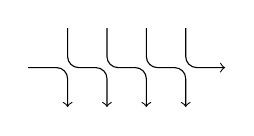
\begin{tikzpicture}
    \draw[->,rounded corners] (0,0) -- (0.5,0) -- (0.5,-0.5);
    \draw[->,rounded corners] (0.5,0.5) -- (0.5,0) -- (1,0) -- (1,-0.5) ;
    \draw[->,rounded corners] (1,0.5) -- (1,0) -- (1.5,0) -- (1.5,-0.5) ;
    \draw[->,rounded corners] (1.5,0.5) -- (1.5,0) -- (2,0) -- (2,-0.5) ;
    \draw[->,rounded corners] (2,0.5) -- (2,0) -- (2.5,0);
    \end{tikzpicture}
\end{center}

By analogy $t(1)^{-1} = \text{cyclic left shift}$. Then 
\eq{
t^{-1}(1) t^\prime(1) &= \sum_i \\
&= \sum_{i=1}^n \check{R}^\prime(1)_{i,i+1} \\
&= AH_{XXZ} + BI
}
where 
\eq{
H_{XXZ} = - \frac{1}{2} \sum_{i=1}^n \pround{\sigma_i^x\sigma_{i+1}^x  + \sigma_i^y \sigma_{i+1}^y  + \frac{1}{2}(q+ q^{-1})\sigma_i^z\sigma_{i+1}^z}
}

\begin{ex}
Show this, finding A,B
\end{ex}
We here are now considering $H_{XXZ}$ as a quantum Hamiltonian for some spin system. \\
Moreover, take $t(\lambda) = t^{(0)} + (\lambda-)t^{(1)} + \dots = \sum_{k=0}^\infty (\lambda -1)^k t^{(k)}$. Then 
\eq{
\comm[t(\lambda)]{t(\lambda^\prime)} = 0 \Rightarrow \comm[t(\lambda)]{t^{(i)}} = 0 \Rightarrow \comm[t^{(i)}]{t^{(j)}}=0
}
and so 
\eq{
\comm[t(\lambda)]{H_{XXZ}} = 0 \Rightarrow \comm[t^{(i)}]{H_{XXZ}} = 0
}
The $t^{(i)}$ are then multiple conserved charges of the theory, giving a quantum analogue of the condition of Liouville integrability. 

%%%%%%%%%%%%%%%%%%%%%%%%%%%%%%%%%%%%%%%%%%%%%%%%%%%%%%%%
\subsection{Comments}
$H_{XXZ}$ is interesting itself, as it is a model of real material which are effectively 1 dimensional, e.g. copper sulphate. We can then use this theory to make real predictions for a laboratory setting. \\
Further, we recall that all physically interesting quantities are written as correlation functions $\pangle{v^\prime \, | \, \mc{O} \, | \, v}$ in quantum field theory. Computing these via quantum integrable structure is possible. 
%%%%%%%%%%%%%%%%%%%%%%%%%%%%%%%%%%%%%%%%%%%%%%%%%%%%%%%%
%%%%%%%%%%%%%%%%%%%%%%%%%%%%%%%%%%%%%%%%%%%%%%%%%%%%%%%%
\bibliographystyle{plain}
\bibliography{references.bib}

\end{document}
